\documentclass[12pt,letterpaper,oneside,final]{book}		
\usepackage[lmargin=3.0cm,rmargin=2.5cm,tmargin=2.5cm,bmargin=2.5cm]{geometry}
\usepackage[table]{xcolor}
\usepackage{setspace}
\usepackage{tabulary}
\usepackage{mfirstuc}
\usepackage{graphicx}
\usepackage{multicol}
\usepackage{multirow}
\usepackage{caption}
\usepackage{float}
\usepackage{wrapfig}
\usepackage{lipsum}
\usepackage{ifpdf}
\usepackage[utf8]{inputenc}
\usepackage[T1]{fontenc}
\usepackage[]{times}
\usepackage[spanish]{babel}
\usepackage[nottoc]{tocbibind}
\usepackage{hyperref}
\usepackage{amsmath,amssymb}
\usepackage{array}
\usepackage{afterpage}
\usepackage{subcaption}
\usepackage{makeidx}
\usepackage{color}
\usepackage{adjustbox}
% \usepackage{refcheck} % checks for unreferenced labels
\usepackage{datetime}
\usepackage{acro}
\usepackage{mfirstuc}% provides \capitalisewords
\usepackage{parskip}
\usepackage{fancyhdr}
\usepackage{listings}

\acsetup{list-long-format=\capitalisewords}

\fancypagestyle{newstyle}{
\fancyhf{} % clear all header and footer fields
\fancyhead[l]{} % except the center
\fancyfoot[R]{\thepage} % except the center
\renewcommand{\headrulewidth}{0pt}
\renewcommand{\footrulewidth}{0pt}}

\pagestyle{newstyle}

% \norefnames % no margin ref names
% \nocitenames % no margin cite names

\makeindex
% \usepackage{showframe}
\ifpdf
  \usepackage{epstopdf}
\fi

\onehalfspacing
\setlength{\parindent}{4em}

\renewcommand\floatpagefraction{.9}
\renewcommand\topfraction{.9}
\renewcommand\bottomfraction{.9}
\renewcommand\textfraction{.1}
\addto\captionsspanish{%
  \renewcommand{\tablename}%
    {Tabla}%
}

\setcounter{totalnumber}{50}
\setcounter{topnumber}{50}
\setcounter{bottomnumber}{50}

% Different font in captions
\newcommand{\captionfonts}{\small}

\makeatletter  % Allow the use of @ in command names
\long\def\@makecaption#1#2{%
  \vskip\abovecaptionskip
  \sbox\@tempboxa{{\captionfonts #1: #2}}%
  \ifdim \wd\@tempboxa >\hsize
    {\captionfonts #1: #2\par}
  \else
    \hbox to\hsize{\hfil\box\@tempboxa\hfil}%
  \fi
  \vskip\belowcaptionskip}
\makeatother   % Cancel the effect of \makeatletter

\hypersetup{
    colorlinks,
    citecolor=black,
    filecolor=black,
    linkcolor=black,
    urlcolor=black
}

\newcommand\blankpage{%
    \null
    \thispagestyle{empty}%
    \addtocounter{page}{-1}%
    \newpage
}

\newcommand{\quotemarks}[1]{``#1''} 

\newdateformat{monthyeardate}{%
  \monthname[\THEMONTH] del \THEYEAR}

\DeclareAcronym{BRDF}{
  short = BRDF,
  long  = función de distribución de reflectancia bidireccional
}
\DeclareAcronym{BSSRDF}{
  short = BSSRDF,
  long  = función de distribución de reflectancia y transluminiscencia bidireccional
}
\DeclareAcronym{NDF}{
  short = NDF,
  long  = función de distribución normal
}
\DeclareAcronym{CLPV}{
  short = CLPV,
  long  = volúmenes de propagación de luz en cascada
}
\DeclareAcronym{LPV}{
  short = LPV,
  long  = volumen de propagación de luz
}
\DeclareAcronym{GV}{
  short = GV,
  long  = volumen de geometría
}
\DeclareAcronym{RSM}{
  short = RSM,
  long  = mapas de sombras reflexivos
}
\DeclareAcronym{VPL}{
  short = VPL,
  long  = luz puntual virtual
}
\DeclareAcronym{GBuffer}{
  short = G-Buffer,
  long  = buffer de geometría
}
\DeclareAcronym{VCT}{
  short = VCT,
  long  = trazado vóxeles con conos
}
\DeclareAcronym{GPU}{
  short = GPU,
  long  = unidad de procesamiento gráfico
}
\DeclareAcronym{GPGPU}{
  short = GPGPU,
  long  = cómputo de propósito general en la unidad de procesamiento gráfico
}
\DeclareAcronym{AABB}{
  short = AABB,
  long  = caja delimitante alineada a los ejes
}



\setcounter{tocdepth}{3}
\setcounter{secnumdepth}{3}

\newcolumntype{R}[2]{%
    >{\adjustbox{angle=#1,lap=\width-(#2)}\bgroup}%
    l%
    <{\egroup}%
}
\newcommand*\rot{\multicolumn{1}{R{60}{1em}}}% no optional argument here, please!
\newcommand\rotv[1]{\rotatebox[origin=c]{90}{#1}}% no optional argument here, please!

\renewcommand{\arraystretch}{1.2}

\lstset{
  language=C++,
  captionpos=b,
  frame=tb,
  tabsize=4,
  breaklines=true,
  basicstyle=\scriptsize\ttfamily,
  keywordstyle=\color{blue}\ttfamily,
  stringstyle=\color{red}\ttfamily,
  commentstyle=\color{green}\ttfamily,
  morecomment=[l][\color{magenta}]{\#},
  escapeinside={(*@}{@*)}
}

\renewcommand{\lstlistingname}{Codigo}

\begin{document}
  \frontmatter
  % portada
  \label{ch:portada}
\thispagestyle{empty}

\begin{figure}[t]
    \centering
    
\includegraphics[height=0.15\textwidth]{media/logoucv.eps}
\end{figure}

\begin{center}
	Universidad Central de Venezuela\\
	Facultad de Ciencias\\
	Escuela de Computaci\'on\\
	Centro de Computaci\'on Gr\'afica\\
\end{center}
				
\vspace{2.5cm}

\begin{center}
	\large{\textbf{Trazado de Conos para el Cálculo de Iluminación\\ Global empleando Sombreado de Vóxeles}}
\end{center}
				
\vspace{2.5cm}

\begin{center}
    Trabajo Especial de Grado presentado ante la Ilustre\\
    Universidad Central de Venezuela \\
    por el Br. José Gabriel Villegas Guedez\\
    para optar al título de Licenciado en Computación.
\end{center}

\vspace{2.5cm}				
				
\begin{center}
	Tutor:\\
	Prof. Esmitt Ramírez
\end{center}
				
\vspace{\fill}

\begin{center}
	Caracas, \monthyeardate\today
\end{center}

\newpage
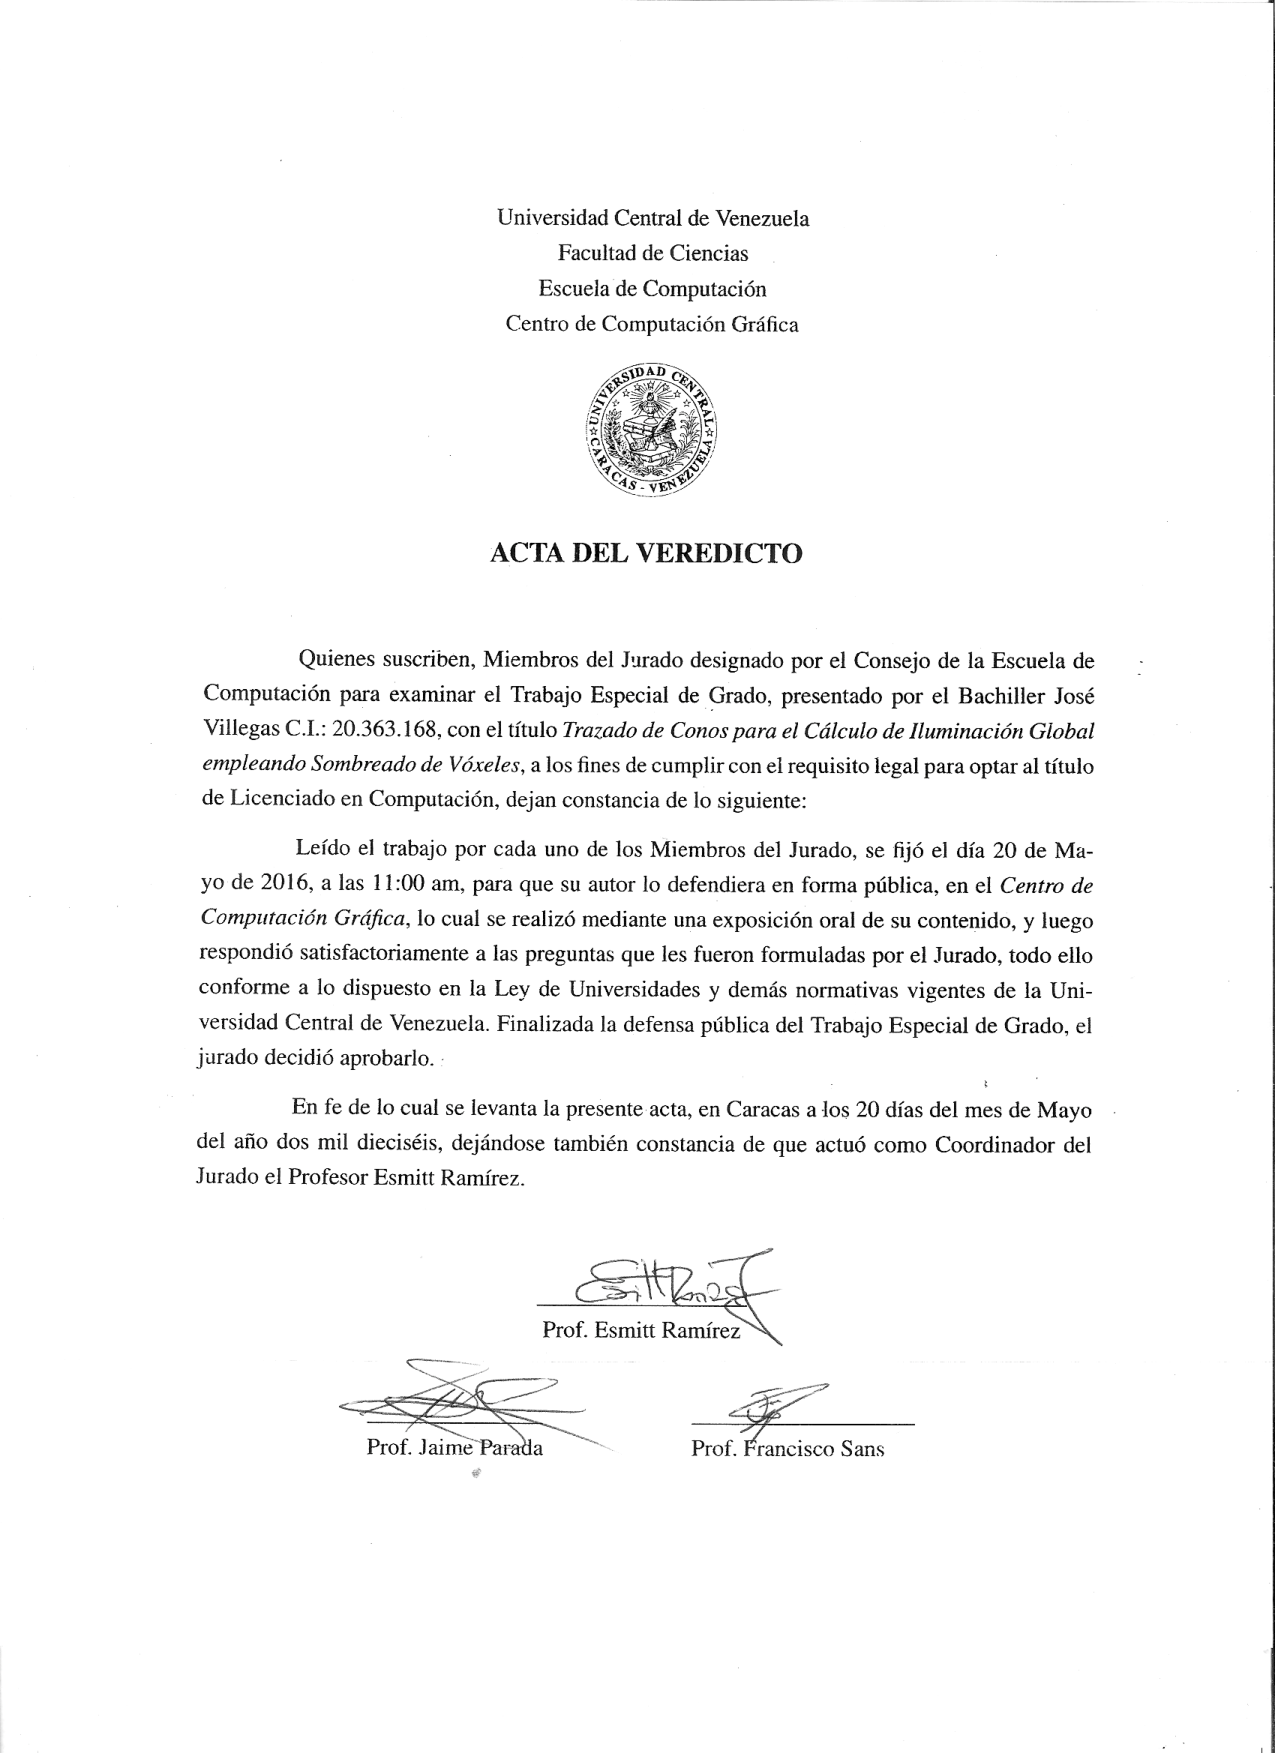
\includepdf{Acta.pdf}			
  % resumen
  \section*{Resumen}
La iluminación de escenas es fundamental para la generación imágenes de alta calidad, esta provee inmersión, sensación de profundidad y realismo. La producción de iluminación realista comprende, entre muchas otras cosas, la inclusión de iluminación indirecta para la composición de iluminación global.

Existen varios algoritmos para el cálculo de la iluminación global de forma analítica, sin embargo el costo computacional de estos es alto y dependiente de la complejidad de la escena. Esto hace estas soluciones poco flexibles o simplemente inadecuadas para aplicaciones en tiempo real, altamente interactivas o de considerable complejidad geométrica. 

Con el incremento de la capacidad de cómputo en las unidades de procesamiento grafico modernas también ha aumentado el interés por la inclusión de fenómenos de iluminación global en aplicaciones en tiempo real. De esto han surgido una variada cantidad de aproximaciones explotando características del hardware de procesamiento gráfico y los recursos disponibles en el pipeline de renderizado. Estos algoritmos mantienen cierto grado de coherencia o convergen con la solución analítica al problema de iluminación global. 

Este trabajo tiene como enfoque principal el renderizado de iluminación global en tiempo real, por esto se realiza una investigación de estos algoritmos y se presenta el desarrollo de una aplicación con iluminación global inspirada principalmente en el trabajo de trazado de vóxeles y conos introducido por Cyril Crassin y otros en 2011.
\paragraph{Palabras Clave:}
Iluminación global, vóxeles, trazado de conos, iluminación indirecta, unidad de cómputo gráfico, renderizado en tiempo real.
  % Tabla de contenido, indice
  \tableofcontents
  % contenido
  % \printacronyms[include-classes=abbrev,name=Abreviaturas]
  \afterpage{\blankpage} % pagina vacia despues del indice
  % introducction
  \addcontentsline{toc}{chapter}{Introducción}
\chapter*{Introducción}
\label{ch:intro}
La síntesis de imágenes realistas siempre ha sido un objetivo de la computación gráfica. La iluminación de escenas es uno de los aspectos importantes para este objetivo. El cálculo preciso de iluminación es un proceso complejo ya que la luz no solo sale de un punto y llega a otro, esta se propaga, rebota y es absorbida por distintos elementos es escena.

En el pipeline de renderizado estándar se utilizan triángulos los cuales son rasterizados para generar fragmentos que luego son coloreados. La representación de superficies en forma de triángulos es efectiva para cálculos como iluminación directa, sin embargo esta posee grandes limitaciones para incorporar fenómenos de iluminación más complejos como iluminación global.

Técnicas recientes han surgido donde se utiliza una representación de la escena en vóxeles para simplificar la geometría en escena y hacer posible el cálculo de iluminación global en tiempo real. Un vóxel representa un elemento volumétrico en una cuadrícula tridimensional uniforme, es también referido como píxel volumétrico o tridimensional.

Una escena representada en vóxeles permite evitar los problemas de complejidad geométrica y su relación con el rendimiento de varias soluciones al problema de iluminación. Esta representación además puede ser filtrada a menores niveles de detalle bajo un esquema de \emph{mipmapping}. 

Estas propiedades son especialmente útiles para el algoritmo de trazado de conos. La complejidad del cálculo de colisión entre geometría poligonal y conos se reduce al aproximar esta al muestreo de un volumen donde según la apertura del cono se utiliza algún nivel de detalle en la estructura de vóxeles.

%\addcontentsline{toc}{section}{Objetivos}
\section*{Objetivos} % (fold)
\label{sec:section_name}
%\addcontentsline{toc}{subsection}{Objetivo General}
\subsection*{Objetivo General} % (fold)
\label{sub:subsection_name}
Desarrollar un método para el cómputo de iluminación global en tiempo real basado en trazado de conos y vóxeles en escenas interactivas.
% subsection subsection_name (end)
%\addcontentsline{toc}{subsection}{Objetivos Específicos}
\subsection*{Objetivos Específicos} % (fold)
\label{sub:objetivo_especifico}
\begin{itemize}
\item Realizar proceso de voxelización de la geometría en escena.
\item Implementar la técnica de \emph{deferred shading}.
\item Implementar una estructura de vóxeles para representar una simplificación de la escena.
\item Construir una descripción jerárquica para esta estructura de vóxeles para almacenar distintos niveles de detalle.
\item Implementar la actualización dinámica de esta estructura al detectar cualquier cambio relevante en escena.
\item Diseñar la representación interna de cada vóxel.
\item Implementar el trazado aproximado de conos contra vóxeles.
\item Garantizar fenómenos de iluminación global como oclusión ambiental e iluminación indirecta.
\item Implementar sombreado de vóxeles para su uso en trazado de conos.
\item Incluir oclusión con sombras para el sombreado de vóxeles.
\item Generar sombras suaves utilizando trazado de conos.
\item Aproximar materiales emisivos con la inclusión de emisión durante el sombreado de vóxeles.
\item Aproximar iluminación indirecta de uno y dos rebotes.
\item Realizar pruebas de rendimiento y precisión sobre diversas escenas y resoluciones.
\end{itemize}
% subsection objetivo_especifico (end)
% section section_name (end)
% \addcontentsline{toc}{section}{Estructura del Documento}
% \section*{Estructura del Documento} % (fold)
% \label{sec:estructura_del_documento}
% Este trabajo está divido en cinco capítulos:
% \begin{itemize}
% \item \textbf{Capítulo 1} provee parte del fondo teórico en iluminación global y su renderizado, la descripción de algunas técnicas utilizadas en este trabajo y un grupo de aproximaciones existentes para el cálculo de iluminación global en tiempo real.
% \item \textbf{Capítulo 2} expone la teoría e ideas asociadas a la propuesta e implementación de este trabajo de forma general.
% \item \textbf{Capítulo 3} detalla los algoritmos implementados y la estructura de la aplicación utilizada para el desarrollo de esta propuesta.
% \item \textbf{Capítulo 4} se estudian distintos entornos de prueba para obtener resultados en cuanto rendimiento y calidad de imagen bajo distintas condiciones en nuestra propuesta.
% \item \textbf{Capítulo 5} se presentan las conclusiones sobre el trabajo realizado y posibles mejoras para trabajos futuros.
% \end{itemize}
% section estructura_del_documento (end)

  % after introduction main matter starts
  \mainmatter
  % marco teorico - global illumination
  \chapter{Marco Teórico}
\label{chap:gi_intro}

\section{Iluminación Global}

Iluminación global se le llama al proceso de calcular la distribución de la energía de la luz sobre escenas tridimensionales desplegadas por computadora. Los efectos de la iluminación global incluyen suave sombreado debajo de objetos y cerca de esquinas, rebotes de luz, mezcla de colores, cáusticas, transluminiscencia, entre otros. Estos efectos son muy sutiles pero afectan el realismo de la imagen final de forma substancial \cite{pixar_renderman_intro}. La figura \ref{fig:gi_comparison} muestra algunos de estos efectos.

\begin{figure}[H]
	\centering
	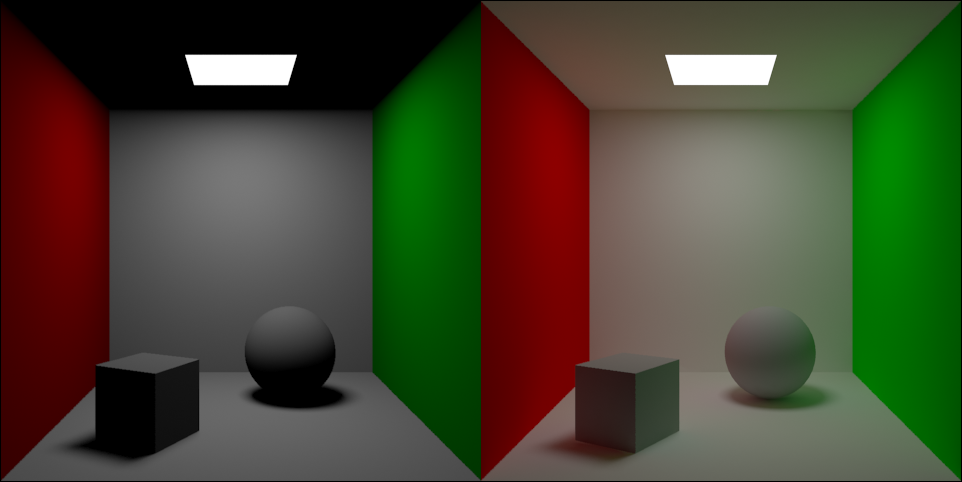
\includegraphics[width=0.985\linewidth]{media/direct_vs_indirect.png}
	\caption{Solo iluminación directa (izquierda). Iluminación global (derecha)}
	\label{fig:gi_comparison}
\end{figure}

El cómputo preciso y completo de iluminación global es considerado poco flexible, costoso y lento para ser utilizable en ciertos medios visuales que requieren producción de imágenes en tiempos interactivos o en escenas de gran complejidad, por ejemplo videojuegos o simulaciones. Es por ello que el desarrollo de aproximaciones y algoritmos para simular iluminación global con mejores factores de rendimiento y flexibilidad es un constante tema de investigación.

\section{Radiometría}
Radiometría es el campo dedicado al estudio y medición de la radiación electromagnética. Para el computo de la distribución de la luz es necesario entender algunas unidades importantes \cite{advanced_gi2006}.

\subsection{Unidades en Radiometría}

\subsubsection{Flujo Radiante}
La unidad fundamental en radiometría, usualmente denotada como $\Phi$ es expresada en watts o vatios. Esta cantidad expresa cuanta energía total fluye desde, hasta y a través de una superficie por unidad de tiempo.
\subsubsection{Irradiancia}
\label{subsubsec:irradiance}
La irradiancia $E$ es el flujo radiante entrante o incidente por unidad sobre el área de una superficie. Esta es expresada en $watts/m^2$:

\begin{equation}
    E = \frac{d\Phi}{dA}
	\label{eq:irradiance_eq}
\end{equation}

\subsubsection{Emitancia Radiante o Radiosidad}
La emitancia radiante $M$ es el flujo radiante saliente o emitido por unidad sobre el área de una superficie. También es expresada en $watts/m^2$:

\begin{equation}
    M = \frac{d\Phi}{dA}
	\label{eq:radiosity_eq}
\end{equation}

\subsubsection{Radiancia}
La radiancia $L$ es el flujo radiante emitido por unidad de ángulo sólido y por unidad de área proyectada, expresada en $watts/estereorradi\acute{a}n\cdot m^2$. De forma intuitiva la radiancia expresa cuanta potencia llega (o sale) de un punto $x$ por unidad de ángulo sólido y por unidad de área proyectada. La radiancia varia con la posición $x$ y el vector dirección $\Theta$, es expresada como $L(x,\Theta)$.

\begin{equation}
    L = \frac{d^2\Phi}{dwdA^\bot} = \frac{d^2\Phi}{dwA\cos\theta}
	\label{eq:radiance_eq}
\end{equation}

\begin{figure}[H]
	\centering
	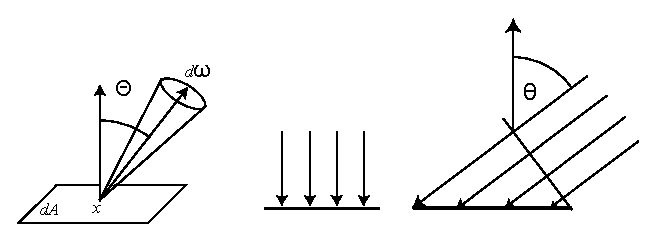
\includegraphics[width=0.85\linewidth]{media/radiance.eps}
	\caption{Definicion de radiancia $L(x,\Theta)$. Flujo radiante emitido por unidad de ángulo solido $dw$ y por unidad de área proyectada $A^\bot$.}
	\label{fig:radiance_fi}
\end{figure}

La radiancia es el término más importantes para los propósitos de este trabajo y probablemente lo es también para una cantidad importante de algoritmos y aproximaciones para el cálculo de iluminación global, es esta unidad la que captura la apariencia de los objetos en escena.

\section{Iluminación directa e indirecta}
\label{sec:direct_indirect}
La iluminación directa es aquella que se proyecta sobre la superficie de algún objeto directamente desde las fuentes de luz en la escena. Iluminación indirecta es la luz que proviene de los subsecuentes rebotes de luz originados desde las superficies iluminadas, ya sea esta superficie reflectiva o no \cite{advanced_gi2006} (Figura \ref{fig:gi_comparison}). La composición de ambas resulta en iluminación global.
\section{Representación de Superficies}
\label{sec:surface_rep}

Los materiales interactúan con la luz de distintas maneras. Esto hace que la apariencia de ciertos materiales difiera según la condiciones de la luz en una escena. Algunos materiales parecen espejos mientras que otros son totalmente difusos. Son visualmente distinguible materiales como vidrio, madera o metales. Las propiedades de reflectancia de una superficie afectan la apariencia del objeto \cite{advanced_gi2006}, estos objetos se distinguen por la cantidad de luz reflectada en ciertas direcciones. 

En el caso más general, un rayo de luz entra en algún punto $p$ sobre una superficie en una escena, este rayo de luz tiene una dirección incidente $\Psi$ y puede salir de esta superficie sobre otro punto $q$ con dirección saliente $\Theta$. La función que define esta relación entre la radiancia incidente y la radiancia reflectada se llama \ac{BSSRDF}.

\subsection{Función de Distribución de Reflectancia Bidireccional}
Al asumir que la luz incidente en algún punto $x$ sale del mismo punto $x$ (ignorando la transluminiscencia) las propiedades de reflectancia de una superficie son entonces descritas por una \ac{BRDF}. En la Figura \ref{fig:bssrdf} se puede observar la diferencia entre \ac{BRDF} y \ac{BSSRDF}.

\begin{figure}[H]
	\centering
	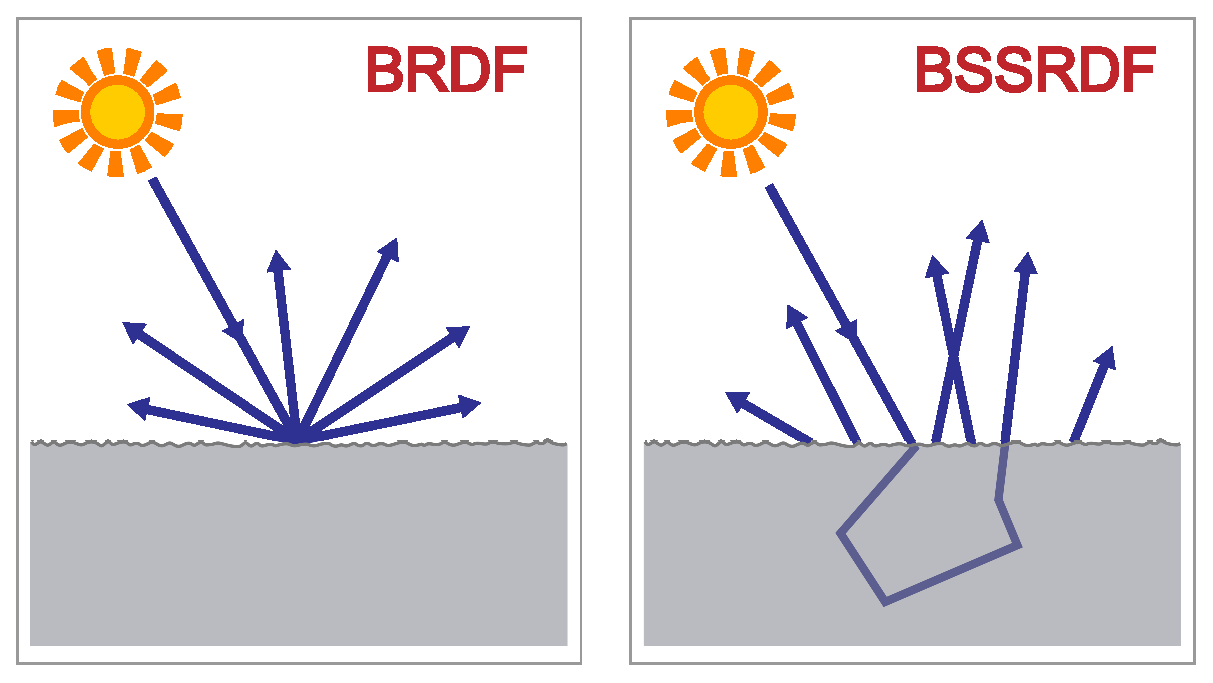
\includegraphics[width=.6\linewidth]{media/brdf_vs.eps}
	\caption
	{
    	Izquierda: BRDF, punto de salida es igual al punto de entrada. Derecha: BSSRDF, se observa como el punto de salida es distinto al de entrada.
	}
	\label{fig:bssrdf}
\end{figure}

La \ac{BRDF} en un punto $x$ se define entonces como la distribución de la radiancia reflectada diferencial en una dirección saliente $\Theta$ y la irradiancia incidente diferencial a través de un ángulo solido $dw_{\Psi}$. La función \ac{BRDF} puede ser escrita de la siguiente forma \cite{advanced_gi2006}:

\begin{equation}
	\begin{split}
        f_{r}(x, \Psi\to\Theta) &= \frac{dL(x\to\Theta)}{dE(x\gets\Psi)}\\
        &= \frac{dL(x\to\Theta)}{L(x\gets\Psi)\cos(N_{x}, \Psi)dw_{\Psi}}
	\end{split}
	\label{eq:brdf_def}
\end{equation} donde $\cos(N_{x}, \Psi)$ es el coseno del ángulo formado entre la normal en el punto $x$ y el vector dirección $\Psi$, también llamado atenuación normal.

\subsubsection{Propiedades de la Función BRDF}

La función BRDF tiene una variada cantidad de importantes propiedades:

\begin{enumerate}
	\item Dimensión: La función BRDF es una función cuatridimensional definida sobre cada punto de una superficie, dos dimensiones corresponden a la dirección entrante y dos a la dirección saliente.
	\item Reciprocidad: El resultado de la función BRDF es el mismo si se intercambian la dirección entrante y la dirección saliente:
    	\begin{equation}
            f_{r}(x, \Psi\to\Theta) = f_{r}(x, \Theta\to\Psi)
    	\end{equation}
	\item Conservación de la energía: La ley de conservación de la energía dicta que la cantidad total de energía reflectada en todas las direcciones debe ser menor o igual a la cantidad de total de energía incidente sobre las superficies: 
    	\begin{equation}
    		\int_{\Omega^{+}}f_{r}(x, \Psi\to\Theta)\cos(N_{x}, \Theta)dw_{\Theta} \leq 1
    	\end{equation}
\end{enumerate}

\subsubsection{Ejemplos de BRDF}
Dependiendo del comportamiento de la \ac{BRDF}, el material se verá como una superficie difusa, como un espejo o como una mezcla de ambos (lustroso o \emph{glossy}). En la Figura \ref{fig:brdf_types} se ilustra estas propiedades. Los tipos de BRDF relevantes para este trabajo serán listados aquí.

\begin{figure}[H]
	\centering
	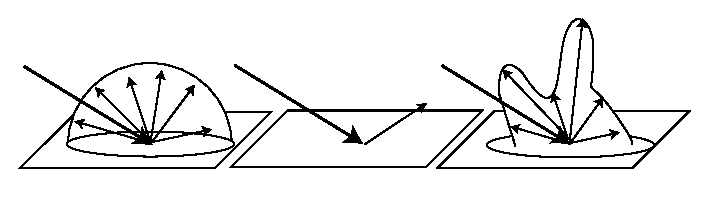
\includegraphics[width=0.85\linewidth]{media/brdfs_types.eps}
	\caption{Ejemplos de superficies: totalmente difusa izquierda, totalmente especular centro, lustrosa (\emph{glossy}) derecha \cite{advanced_gi2006}.}
	\label{fig:brdf_types}
\end{figure}

\paragraph{Superficies Difusas:}
Algunos materiales reflectan la luz de forma uniforme sobre la totalidad de la semiesfera de reflectancia. Esto quiere decir que según la distribución de la irradiancia, la radiancia reflectada es independiente de la dirección de salida. Estos materiales son llamados reflectores difusos y el valor de su \ac{BRDF} es una constante para todos los valores $\Theta$ y $\Psi$. Para un observador un punto sobre una superficie difusa se ve igual desde todas las direcciones \cite{advanced_gi2006}. Para una superficie difusa ideal, la reflexión difusa puede ser representada como:

\begin{equation}
    f_{r}(x, \Psi\leftrightarrow\Theta) = \frac{\rho_{d}}{\pi}
    \label{eq:diffuse_reflection}
\end{equation}

La reflectancia $\rho_{d}$ representa la fracción de la energía incidente que es reflectada en la superficie. Para materiales físicamente correctos, $\rho_{d}$ varía entre 0 y 1.

\paragraph{Superficies Especulares:}
\label{para:speculars}
Superficies especulares perfectas solo reflejan o refractan luz en una dirección específica.
\paragraph{Reflexión Especular:}
La dirección de reflexión puede ser obtenida utilizando la ley de reflexión, esta indica que la dirección de la luz incidente y saliente tienen un ángulo equivalente con la normal de la superficie. Dado que la luz es incidente con respecto a la superficie con vector dirección $\Psi$, y la normal de la superficie es $N$, la luz incidente es reflectada en la dirección $R$:

\begin{equation}
    R = 2(N\cdot\Psi)N - \Psi
    \label{eq:reflectance_direction}
\end{equation}

Un reflector especular perfecto tiene solo una dirección de salida donde la \ac{BRDF} es diferente de $0$, esto implica que el valor de la \ac{BRDF} en esa dirección es infinito.

\paragraph{Superficies Lustrosas:}
La mayoría de las superficies no son ni idealmente difusas ni idealmente especulares, sino que demuestran una combinación de ambas características de reflectancia. Estas superficies son llamadas superficies lustrosas o superficies \emph{glossy}. La \ac{BRDF} que describe esta clase de materiales es usualmente difícil de modelar de forma analítica \cite{advanced_gi2006}.

\subsubsection{Modelos de sombreado.}
Materiales reales puede tener \ac{BRDF}s particularmente complejas. En computación gráfica existen varios modelos que intentan capturar la complejidad de las \ac{BRDF}s. En la siguiente sección se expande sobre ciertos modelos relevantes a este trabajo. Nótese que $\Psi$ es la dirección de la luz (dirección incidente), $\Theta$ es la dirección del observador (dirección saliente) y $N$ la normal de la superficie.

\paragraph{Modelo de Lambert:}
Uno de los modelos más simples, este modelo es ideal para superficies difusas, en este modelo la \ac{BRDF} es una constante como ya fue descrito anteriormente en la ecuación \ref{eq:diffuse_reflection}.

\begin{equation}
    f_{r}(x, \Psi\leftrightarrow\Theta) = k_{d} = \frac{\rho_{d}}{\pi}
    \label{eq:lambert}
\end{equation} donde $\rho_{d}$ es la reflexión difusa.

\paragraph{Modelo de Phong:}
La \ac{BRDF} del modelo de Phong es:

\begin{equation}
    f_{r}(x, \Psi\leftrightarrow\Theta) = k_{s}\frac{(R\cdot \Theta)^n}{N\cdot\Psi} + k_{d}
    \label{eq:phong}
\end{equation} donde el vector reflectado $R$ es calculado con la ecuación \ref{eq:reflectance_direction}.

\paragraph{Modelo de Blinn-Phong:}
\label{para:blinn_phong}
El modelo Blinn-Phong utiliza el vector medio $H$ entre $\Psi$ y $\Theta$ de la siguiente manera:

\begin{equation}
    f_{r}(x, \Psi\leftrightarrow\Theta) = k_{s}\frac{(N\cdot H)^n}{N\cdot\Psi} + k_{d}
    \label{eq:blinn_phong_pr}
\end{equation}

El valor $n$ varía según las propiedades del material. Un mayor valor provee un lóbulo especular más pequeño, simulando superficies lisas y pulidas. En la Figura \ref{fig:blinn_spec_comparison} se puede observar este efecto. En la Figura \ref{fig:brdfs_comparison} se puede observar el resultado de este modelo.

\begin{figure}[H]
	\centering
	\begin{subfigure}[t]{0.25\textwidth}
		\centering
		\captionsetup{justification=centering}
		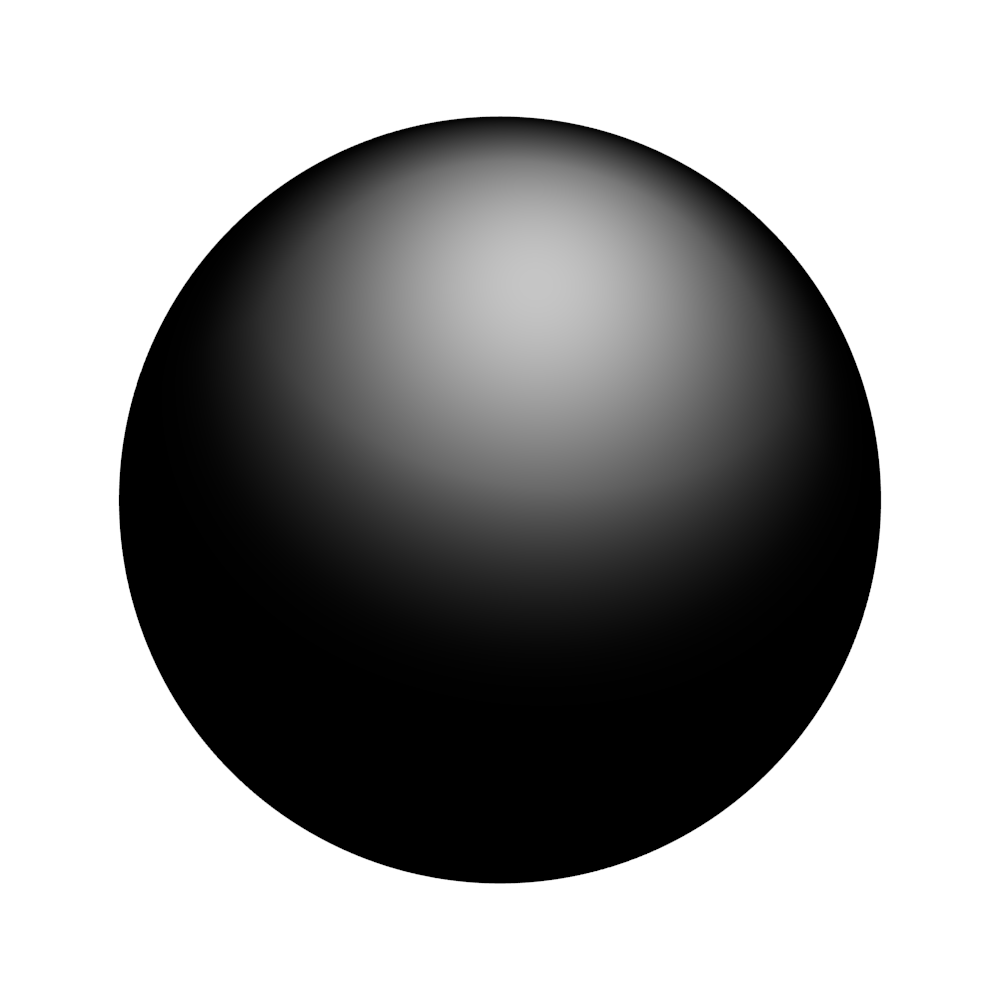
\includegraphics[width=\linewidth]{media/blinn_10.png}
		\caption*{$n = 10$}
	\end{subfigure}%
	\begin{subfigure}[t]{0.25\textwidth}
		\centering
		\captionsetup{justification=centering}
		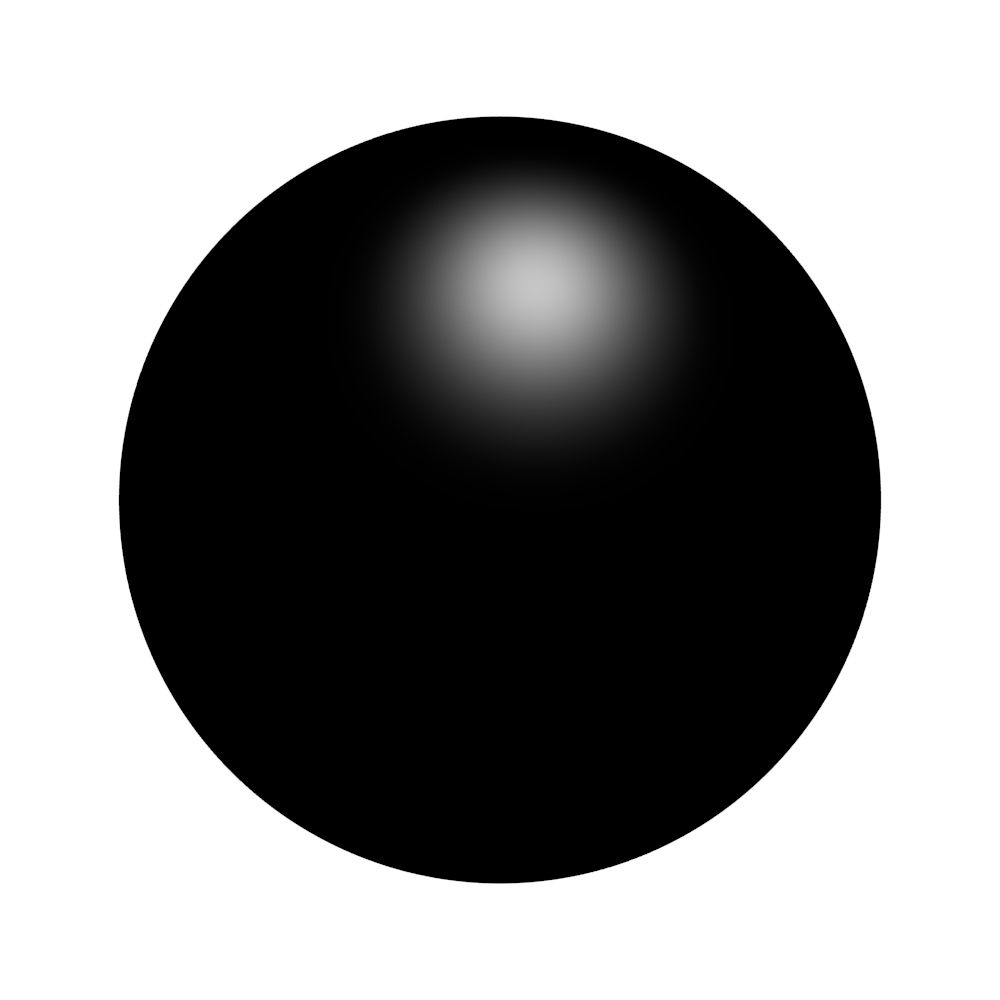
\includegraphics[width=\linewidth]{media/blinn_50.png}
		\caption*{$n = 50$}
	\end{subfigure}%
	\begin{subfigure}[t]{0.25\textwidth}
		\centering
		\captionsetup{justification=centering}
		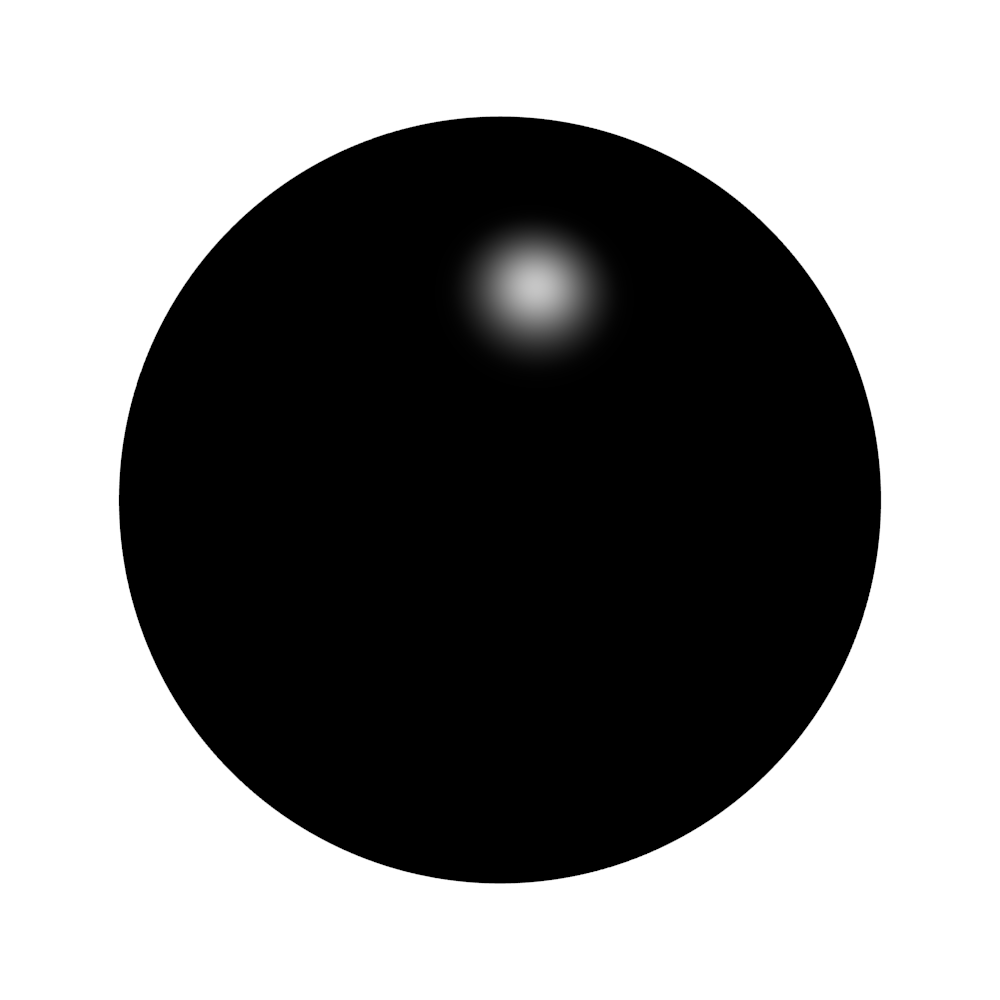
\includegraphics[width=\linewidth]{media/blinn_150.png}
		\caption*{$n = 150$}
	\end{subfigure}%
	\begin{subfigure}[t]{0.25\textwidth}
		\centering
		\captionsetup{justification=centering}
		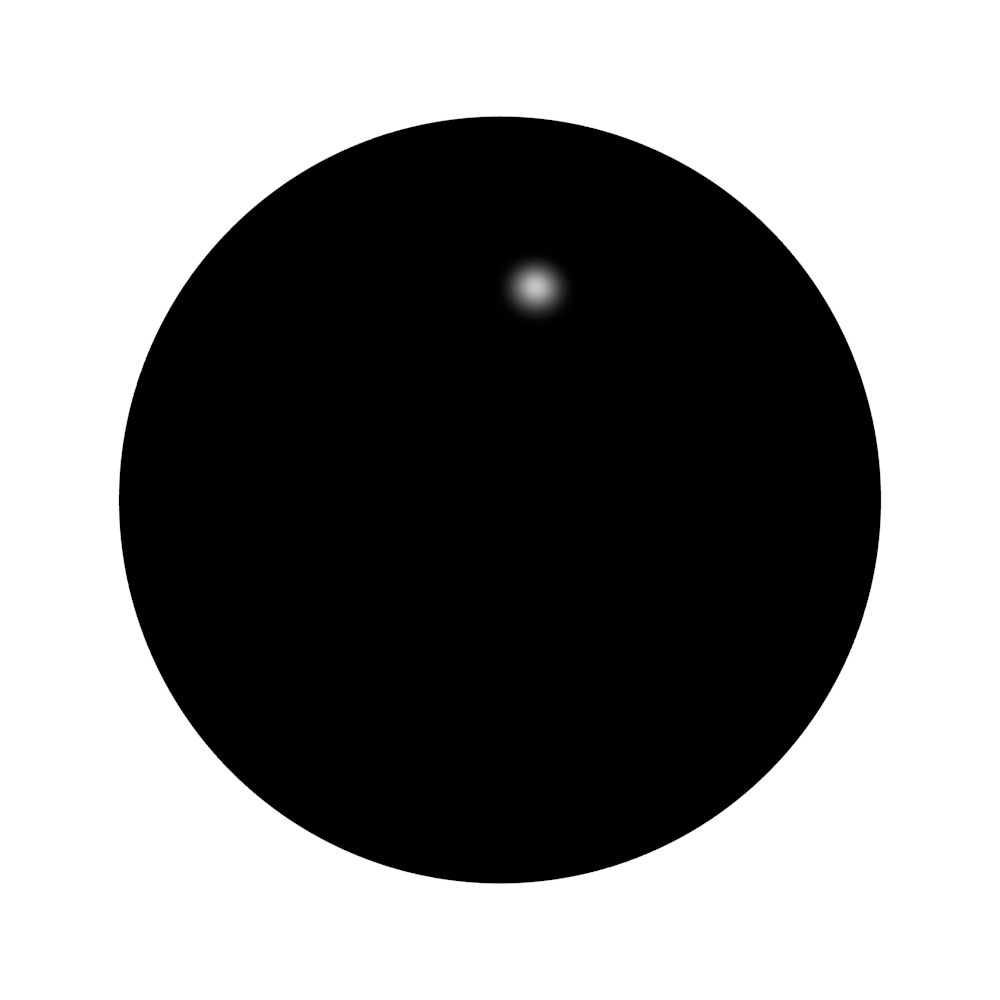
\includegraphics[width=\linewidth]{media/blinn_350.png}
		\caption*{$n = 350$}
	\end{subfigure}%
	\caption{Distribución especular para distintos valores de $n$ en el modelo Blinn-Phong.}
	\label{fig:blinn_spec_comparison}
\end{figure}

\paragraph{Modelo de Blinn-Phong Modificado:}
\label{para:blinn_phong_mod}
El modelo de Phong a pesar de ser simple este tiene ciertas limitaciones, no es ni conservador de energía ni reciproco y tiene problemas para simular materiales reales. El modelo modificado toma en cuenta algunos de estos problemas:

\begin{equation}
    f_{r}(x, \Psi\leftrightarrow\Theta) = k_{s}(N\cdot H)^n + k_{d}
    \label{eq:blinn_phong}
\end{equation}

\begin{figure}[H]
	\centering
	\begin{subfigure}[t]{0.33\textwidth}
		\centering
		\captionsetup{justification=centering}
		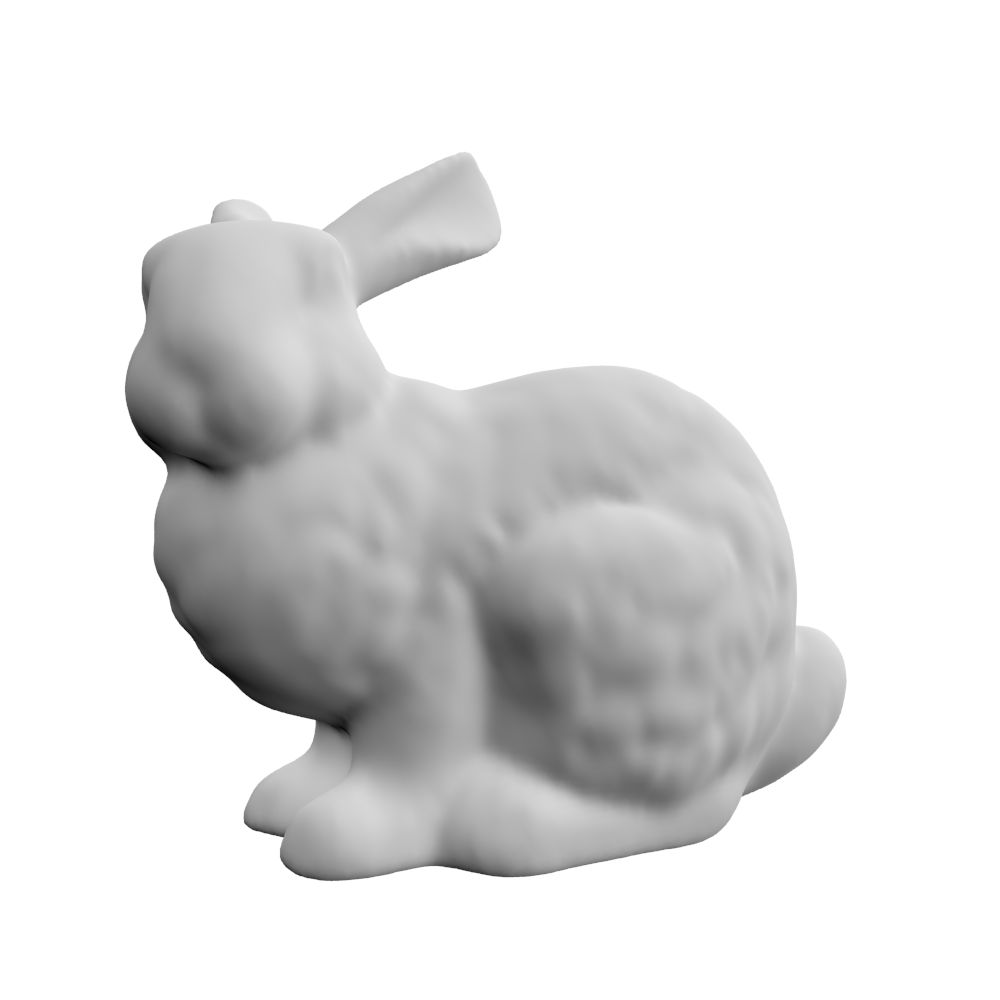
\includegraphics[width=\linewidth]{media/diffuse_bunny.png}
		\caption*{Lambert \ac{BRDF}}
	\end{subfigure}%
	\begin{subfigure}[t]{0.33\textwidth}
		\centering
		\captionsetup{justification=centering}
		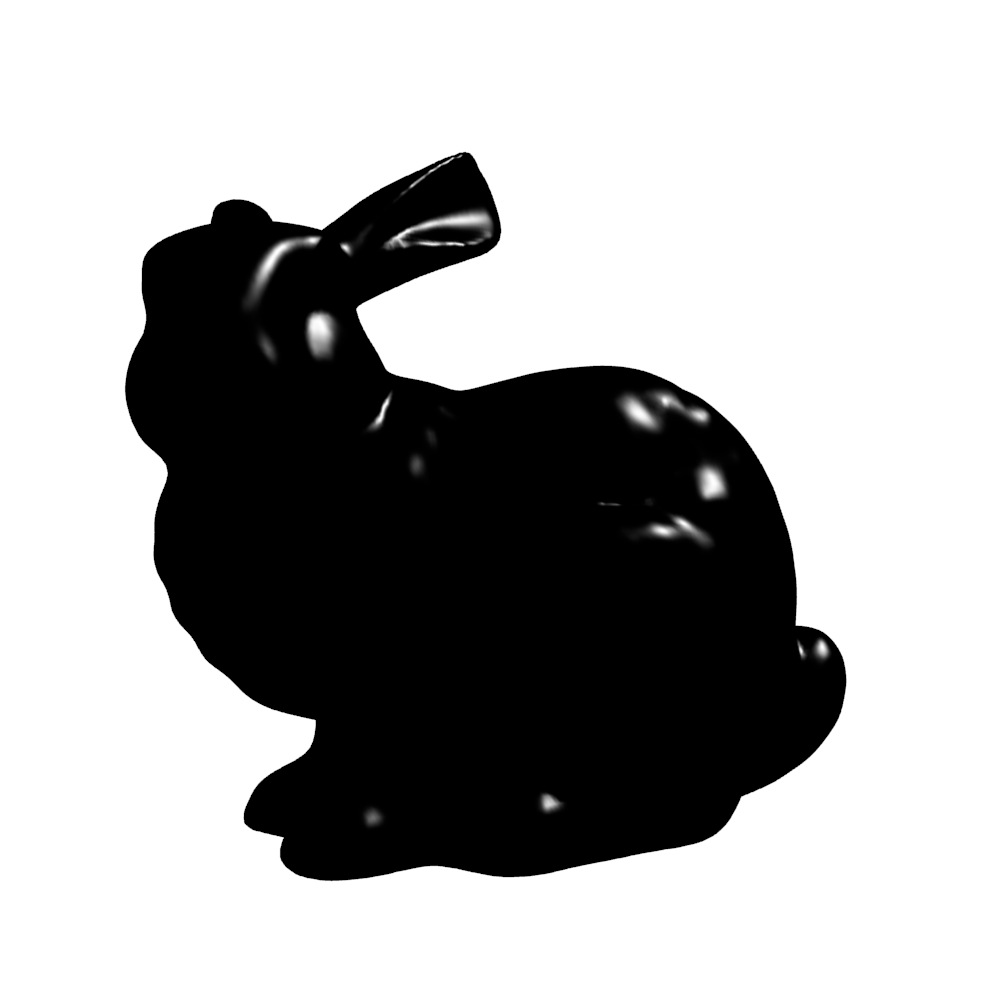
\includegraphics[width=\linewidth]{media/specular_bunny.png}
		\caption*{Blinn-Phong \ac{BRDF}\\ especular}
	\end{subfigure}%
	\begin{subfigure}[t]{0.33\textwidth}
		\centering
		\captionsetup{justification=centering}
		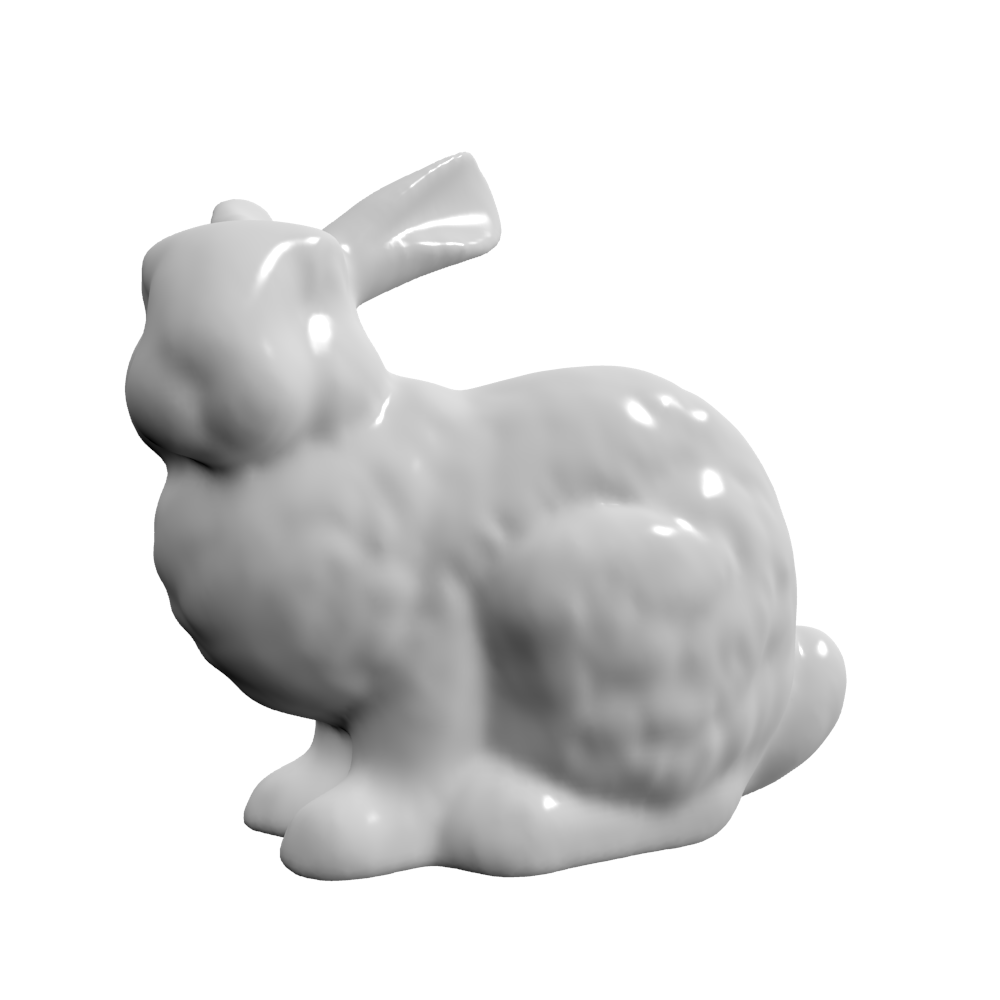
\includegraphics[width=\linewidth]{media/diffuse_specular_bunny.png}
		\caption*{Lambert \ac{BRDF} y \\Blinn-Phong \ac{BRDF} especular.}
	\end{subfigure}
	\caption{Composición de Blinn-Phong y Lambert. Se observa como estas afectan la apariencia final de la superficie.}
	\label{fig:brdfs_comparison}
\end{figure}

\subsection{Función de Distribución Normal}
La \ac{NDF} introducida por Alain Fournier \cite{fournier1992d} describe la densidad de las normales como una función de dirección. Funciones gaussianas como la siguiente es una de las posibles formas de una \ac{NDF}.
\begin{equation}
    f(x) = \frac{1}{\sigma\sqrt{2\pi}}e^{-\frac{(x-\mu)^2}{2\sigma^2}}
    \label{eq:ndf_ex1}
\end{equation}

En la función gaussiana el término $\sigma^2$ es llamado variancia y el término $\mu$ es llamado media. Tanto el producto como la convolución de dos distribuciones gaussianas es también una distribución gaussiana \cite{tina-2003}.

La función gaussiana puede ser utilizada como una representación direccional. En este caso la media es un vector promedio $D$ del lóbulo gaussiano. Como es descrito en el trabajo de Toksvig para el mipmapping de mapas de normales \cite{Toksvig05}, el valor de $\sigma$ puede ser calculado por la longitud del vector promedio $D$ utilizando la siguiente ecuación:
\begin{equation}
    \sigma^2 = \frac{1-|D|}{|D|}
    \label{eq:gaussia_eq}
\end{equation}

Esto permite obtener lóbulos gaussianos a partir de dos o más vectores para representar su dirección en común. En la Figura \ref{fig:brdf_lobules} se puede observar el lóbulo para una distribución de dos direcciones.

\begin{figure}[H]
	\centering
	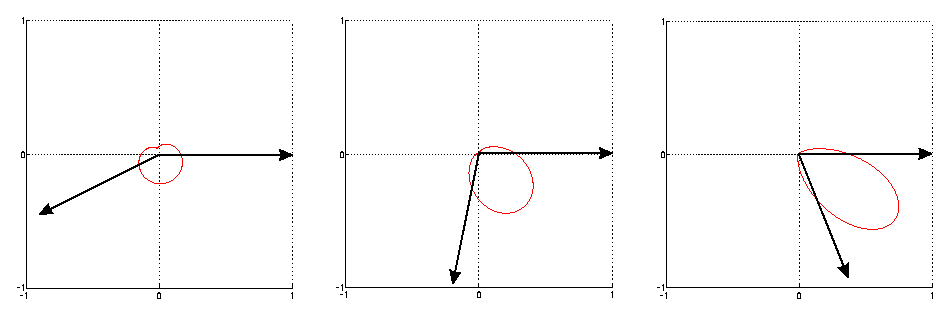
\includegraphics[width=0.85\linewidth]{media/lobes.eps}
	\caption{Ejemplo de lóbulos gaussianos según dos vectores, se puede observar como la forma del lóbulo cambia según la dirección promedio.}
	\label{fig:lobes_example}
\end{figure}

Algunas \ac{BRDF} también pueden describirse como distribuciones gaussianas, las propiedades de producto y convolución se mantienen. Esto se puede observar en la Figura \ref{fig:brdf_lobules}.

\begin{figure}[H]
	\centering
	\begin{subfigure}[t]{0.3\textwidth}
		\centering
		\captionsetup{justification=centering}
		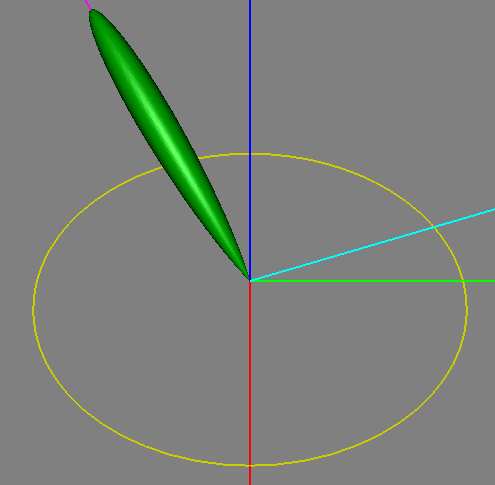
\includegraphics[width=\linewidth]{media/phong_lobule.png}
		\caption*{\ac{BRDF} Phong}
	\end{subfigure}\hfill
	\begin{subfigure}[t]{0.35\textwidth}
		\centering
		\captionsetup{justification=centering}
		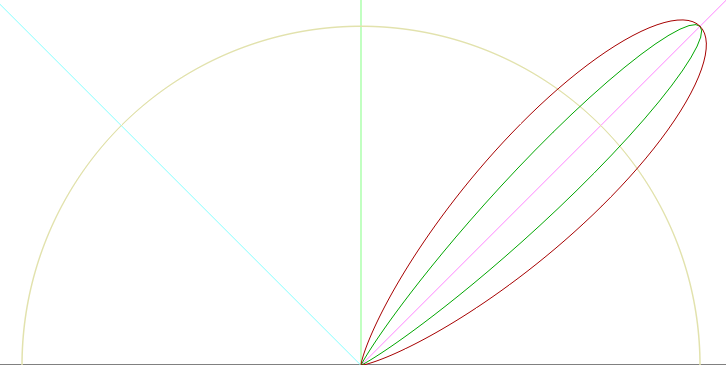
\includegraphics[width=\linewidth]{media/BlinnPhonglobules.png}
		\caption*{Gráfica de ambas en coordenadas polares.}
	\end{subfigure}\hfill
	\begin{subfigure}[t]{0.3\textwidth}
		\centering
		\captionsetup{justification=centering}
		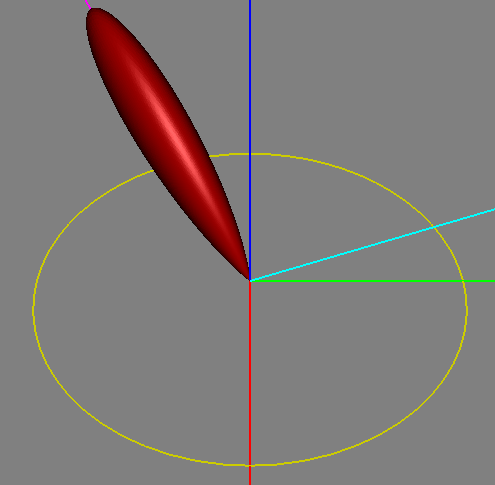
\includegraphics[width=\linewidth]{media/blinnphong_lobule.png}
		\caption*{\ac{BRDF} Blinn-Phong}
	\end{subfigure}\hfill
	\caption{Lóbulos especulares para BRDF Phong y Blinn-Phong para un $\Theta$ y $\Psi$ de $\angle 45$, se puede observar cómo estas describen la distribución de la dirección de reflectancia. Como se explica en \ref{para:blinn_phong} el valor de $n$ afecta la forma del lóbulo mientras mayor es este número más fino y largo es el lóbulo especular. Imágenes renderizadas en Disney's BRDF Explorer \cite{brdf_explorer}.}
	\label{fig:brdf_lobules}
\end{figure}

\section{Ecuación de Renderizado}
La ecuación de renderizado recursiva, introducida por Kajiya \cite{kajiya86}. La ecuacion de renderizado describe en cada punto $x$ de una superficie y en cada dirección $\Theta$, la radiancia saliente $L(x\to\Theta)$ en ese punto y esa dirección.

El objetivo de un algoritmo para el cálculo de iluminación global es aproximar el resultado de esta ecuación. En esta ecuación asumimos que no existen medios participantes como objetos translúcidos como ya fue explicado en la sección \ref{sec:surface_rep}. También asumimos que la luz se propaga de forma inmediata por tanto la distribución de la luz, ya en un estado estacionario, se obtiene inmediatamente. 

\subsection{Formulación Hemisférica}
La formulación hemisférica de la ecuación de renderizado es una de las más utilizadas \cite{advanced_gi2006}. Esta formulación se obtiene utilizando la propiedad de conservación de energía en el punto $x$. Asumiendo que $L_{e}(x\to\Theta)$ representa la radiancia emitida por la superficie en el punto $x$ con dirección saliente $\Theta$ y $L_{r}(x\to\Theta)$ representa la radiancia reflectada por la superficie en el punto $x$ con dirección $\Theta$.

Por conservación de energía, el total de la radiancia saliente en un punto y dirección particular es la suma de la radiancia emitida y la radiancia reflectada en este punto de la superficie y dirección. La radiancia saliente $L(x\to\Theta)$ es expresada en términos de $L_{e}(x\to\Theta)$ y $L_{e}(x\to\Theta)$ de la siguiente forma:
\begin{equation}
    L(x\to\Theta) = L_{e}(x\to\Theta) + L_{r}(x\to\Theta)
    \label{eq:reflectance}
\end{equation}
Por la definición de \ac{BRDF} en la ecuación \ref{eq:brdf_def} tenemos que:
\begin{equation}
	\begin{split}
        f_{r}(x, \Psi\to\Theta) &= \frac{dL(x\to\Theta)}{dE(x\gets\Psi)}\\
        L_{r}(x\to\Theta) &= \int_{\Omega_{x}}{f_{r}(x, \Psi\to\Theta)L(x\gets\Psi)\cos(N_{x}, \Psi)dw_{\Psi}}
	\end{split}
	\label{eq:rendering_eq_LR}
\end{equation}
Colocando estas ecuaciones juntas obtenemos la ecuación de renderizado:
\begin{equation}
    L(x\to\Theta) = L_{e}(x\to\Theta) + \int_{\Omega_{x}}{f_{r}(x, \Psi\to\Theta)L(x\gets\Psi)\cos(N_{x}, \Psi)dw_{\Psi}}
    \label{eq:rendering_eq}
\end{equation}

\subsection{Procedimientos}
En esta sección se explica dos populares procedimientos clásicos para obtener una aproximación a la ecuación de renderizado, esto es una aproximación de la propagación de la luz en una escena. Estas soluciones no están pensadas para tiempos interactivos y su enfoque principal es precisión.

Métodos como elementos finitos y Monte Carlo son los grupos de algoritmos más utilizados para aproximar la ecuación de renderizado. El método de elementos finitos utiliza alguna forma de discretización para reducir la ecuación de renderizado a una ecuación de matrices. Los métodos Monte Carlo muestrean los caminos que siguen los rayos de luz en una escena, generando un estimado estadístico de la apariencia real de la escena. \emph{Radiosity} es una popular aproximación que utiliza el método de elementos finitos. Trazado de rayos y caminos (\emph{ray tracing y path tracing}) son aproximaciones comunes que utilizan el método Monte Carlo \cite{gi_renderingeq}. 

\begin{figure}[H]
	\centering
	\begin{subfigure}{0.24\textwidth}
		\centering
		\captionsetup{width=0.95\textwidth, justification=centering}
		\caption*{Vista desde patch $\alpha$,\\ antes de pasada 1.}
		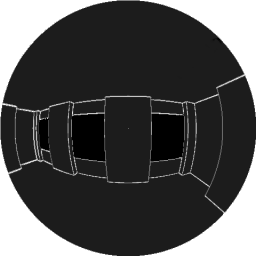
\includegraphics[width=.95\linewidth]{media/radiosity1_eye.png}
	\end{subfigure}
	\begin{subfigure}{0.24\textwidth}
		\centering
		\captionsetup{width=0.95\textwidth, justification=centering}
		\caption*{Patch $\beta$ debajo de $\alpha$,\\ se observa el sol.}
		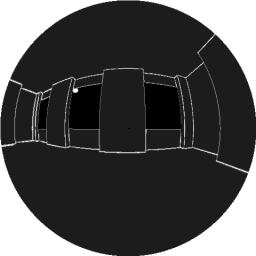
\includegraphics[width=.95\linewidth]{media/radiosity1_eye1.png}
	\end{subfigure}%
	\begin{subfigure}{0.24\textwidth}
		\centering
		\captionsetup{width=0.95\textwidth, justification=centering}
		\caption*{Patches iluminados,\\ durante pasada 1.}
		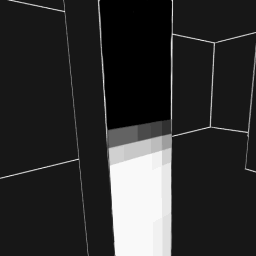
\includegraphics[width=.95\linewidth]{media/radiosity_patch2.png}
	\end{subfigure}%
	\begin{subfigure}{0.24\textwidth}
		\centering
		\captionsetup{width=0.95\textwidth, justification=centering}
		\caption*{Vista desde patch $\alpha$,\\ después de pasada 1.}
		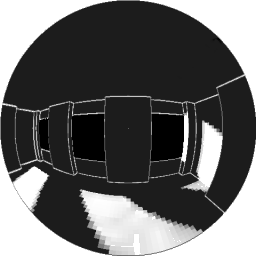
\includegraphics[width=.95\linewidth]{media/radiosity2_eye.png}
	\end{subfigure}
	\label{fig:radiosity1}
\end{figure}%
\begin{figure}[H]
	\centering
	\begin{subfigure}{0.24\textwidth}
		\centering
		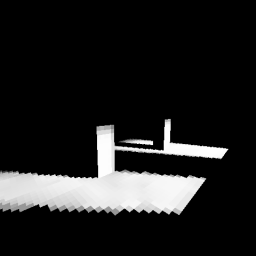
\includegraphics[width=.95\linewidth]{media/radiosity1.png}
		\captionsetup{width=0.95\textwidth, justification=centering}
		\caption*{Pasada 1.}
	\end{subfigure}%
	\begin{subfigure}{0.24\textwidth}
		\centering
		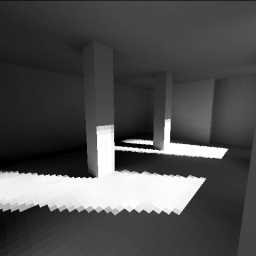
\includegraphics[width=.95\linewidth]{media/radiosity2.png}
		\captionsetup{width=0.95\textwidth, justification=centering}
		\caption*{Pasada 2.}
	\end{subfigure}%
	\begin{subfigure}{0.24\textwidth}
		\centering
		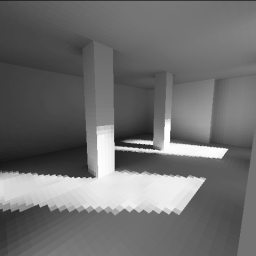
\includegraphics[width=.95\linewidth]{media/radiosity3.png}
		\captionsetup{width=0.95\textwidth, justification=centering}
		\caption*{Pasada 3.}
	\end{subfigure}
	\begin{subfigure}{0.24\textwidth}
		\centering
		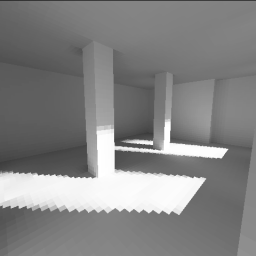
\includegraphics[width=.95\linewidth]{media/radiosity16.png}
		\captionsetup{width=0.95\textwidth, justification=centering}
		\caption*{Pasada 16.}
	\end{subfigure}
	\caption{Ejemplo de varias pasadas de radiosidad sobre una escena. Fuente: Hugo Elias, \emph{The Workings of a Radiosity Renderer} \cite{hugo2000}.}
	\label{fig:radiosity2}
\end{figure}


\subsubsection{Radiosidad}
\label{subsec:radiosity}

Radiosidad es una aproximación con elementos finitos común para el cómputo del transporte de luz global. Esta técnica fue introducida por Goral y otros en 1984 \cite{goral84}. La idea general es discretizar las superficies de la escena en elementos finitos de éstas, estos elementos son usualmente llamados \emph{patches} (parches o trozos) los cuales son utilizados para calcular el transporte de luz entre ellos como se observa en la figura \ref{fig:radiosity2}. Esto conlleva a ciertas implicaciones; de cada \emph{patch} se necesita guardar el valor de radiosidad para las superficies difusas, o la distribución direccional de la luz saliente y entrante para superficies no difusas.

\subsubsection{Trazado de Rayos e Integración Monte Carlo}
\label{subsec:monte_carlo_raytracing}
La ecuación de renderizado puede ser aproximada utilizando el algoritmo de trazado de rayos o \emph{ray tracing}, esta es una técnica basada en integración Monte Carlo. Para aproximar la propagación de la luz se crea un número considerable de muestras en variadas direcciones, luego por cada muestra se evalúa la ecuación de renderizado y el promedio de todos los resultados converge hacia la solución analítica de la ecuación de renderizado. Para evaluar una muestra la luz incidente desde una dirección tiene que ser calculada, para esto un rayo de luz es enviado en una dirección y la luz emitida desde el primer punto de colisión es calculada evaluando la ecuación de renderizado en este punto.

Ray tracing está dividido en dos categorías: forward y backward. Forward ray tracing consiste en lanzar las trazas/rayos de luz desde las fuentes de luz y usar aquellos que llegan a la cámara. Backward ray tracing por el contrario lanza las trazas/rayos de luz desde la cámara y traza el camino de estos a través de la escena \cite{Arvo86backwardray}.

\begin{figure}[H]
	\centering
	\begin{subfigure}{0.33\textwidth}
		\centering
		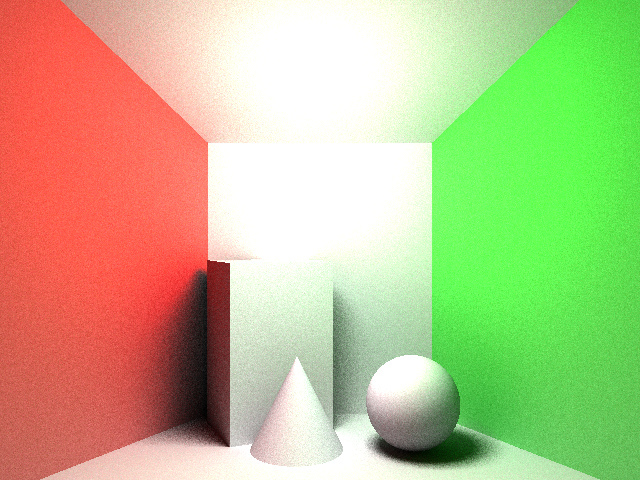
\includegraphics[width=.98\linewidth]{media/ray_100s.jpg}
		\captionsetup{width=0.98\textwidth, justification=centering}
		\caption*{100 muestras rayos/píxel,\\ 50 para luces de área.}
	\end{subfigure}%
	\begin{subfigure}{0.33\textwidth}
		\centering
		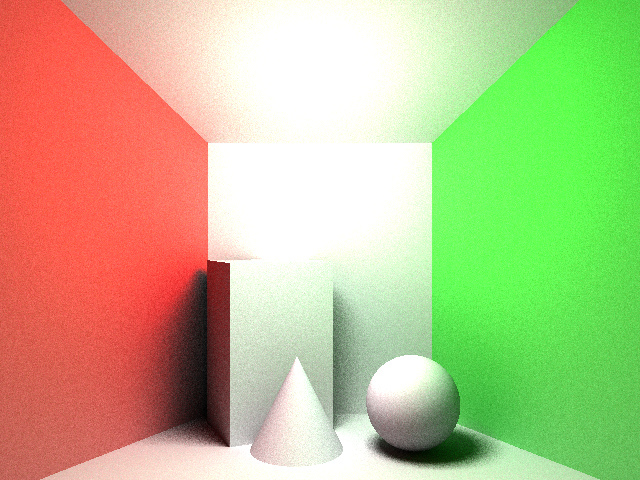
\includegraphics[width=.98\linewidth]{media/ray_500s.jpg}
		\captionsetup{width=0.98\textwidth, justification=centering}
		\caption*{500 muestras rayos/píxel,\\ 50 para luces de área.}
	\end{subfigure}%
	\begin{subfigure}{0.33\textwidth}
		\centering
		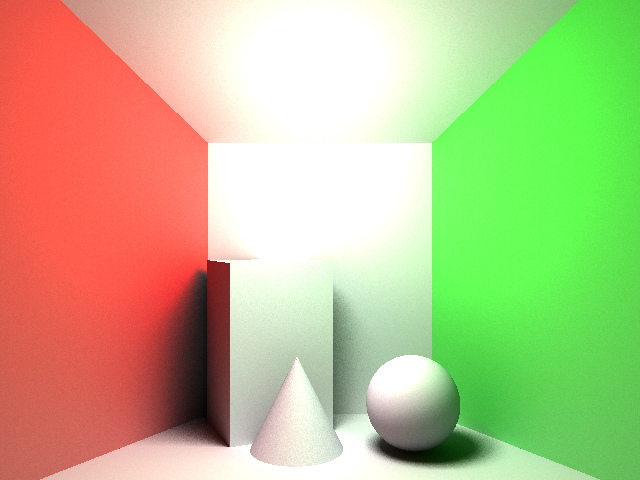
\includegraphics[width=.98\linewidth]{media/ray_1000s.jpg}
		\captionsetup{width=0.98\textwidth, justification=centering}
		\caption*{1000 muestras rayos/píxel,\\ 100 para luces de área.}
	\end{subfigure}
	\caption{Ray tracing sobre una escena, se puede observar mayor calidad y reducción de ruido al aumentar la cantidad de muestras. Fuente: Loc Do, \emph{HW6: Ray Tracing Extension} \cite{locdoraytracing}.}
	\label{fig:ray_tracing_nsamples}
\end{figure}
\section{Técnicas Comunes en Renderizado de Imágenes}

En esta sección se explican técnicas comunes utilizadas en síntesis o renderizado de imágenes que son relevantes para este trabajo.
\subsection{Mapeado de Sombras}
\label{subsec:shadowmapping}
Con la luz representada en forma de rayos las superficies sombreadas reciben menos rayos de luz ya que estas están ocluidas por otras superficies que se encuentra entre ellas y los emisores de luz. En el pipeline de renderizado estándar, donde las superficies en escenas son representadas en geometría poligonal, trazar rayos por cada fragmento para comprobar la visibilidad del mismo no es una operación trivial.

Los mapas de sombras, presentados inicialmente por Lance Williams en 1978 \cite{Williams:78} son una solución simple para el cálculo de visibilidad de un fragmento. La técnica consiste en proyectar la escena en una textura bidimensional desde la posición y con la dirección de una fuente de luz. La proyección es calculada utilizando una matriz de proyección $P_{l}$. Por cada píxel de esta textura la profundidad de cada fragmento sobre una superficie es almacenada. Esta textura es llamada mapa de sombra.

Una vez que se procede a renderizar la escena desde el punto de vista del observador, por cada fragmento con posición $p_{ws}$ en espacio de mundo, la posición en el mapa de sombra $p_{sh}$ es calculada utilizando la siguiente ecuación:
\begin{equation}
    p_{sh} = P_{l} \cdot p_{ws}
    \label{eq:p_to_shadowmap}
\end{equation}
\begin{figure}[H]
	\centering
	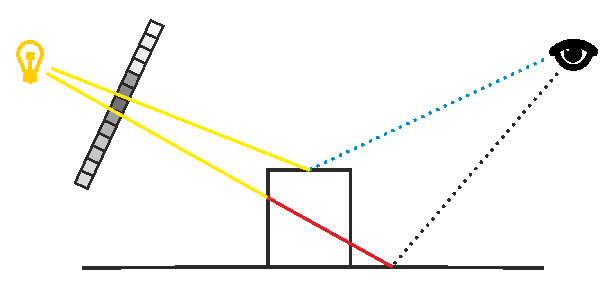
\includegraphics[width=0.80\linewidth]{media/shadow_mapping.eps}
	\caption{La profundidad almacenada en el mapa de sombra (amarillo) es comparada con la profundidad del punto en la superficie desde la luz (rojo).}
	\label{fig:shadow_mapping}
\end{figure}
Como se muestra en la Figura \ref{fig:shadow_mapping}, si la profundidad del fragmento desde la fuente de luz es mayor que el valor almacenado en el mapa de sombra entonces este punto esta sombreado. 

El mapeado de sombras es una solución sencilla y efectiva al problema de pruebas de visibilidad pero esta técnica tiene dos mayores desventajas. El mapa de sombras está limitado a la resolución de la textura y además este representa una discretización de la profundidad de la escena desde la fuente de luz y esto introduce una variedad de anomalías visuales. A partir de este concepto existe una variedad de algoritmos para el cálculo de sombras que intentan solventar estos problemas.

\subsection{Sombreado Diferido}
\label{sub:deferred_rendering_theory}
En sombreado directo la representación poligonal de la escena es rasterizada y operaciones por píxel como iluminación y sombreado son realizadas por cada fragmento generado por el proceso de rasterización. Esto es poco efectivo cuando consideramos que gran parte de los fragmentos no forman parte de la imagen final.
Con sombreado diferido se pueden realizar estas operaciones por píxel solo sobre los fragmentos visibles. Este concepto está basado en el trabajo de Deering et al. en 1998 \cite{Deering:1988}. La escena es renderizada solo una vez y varios atributos de la escena son almacenados en buffers. Este buffer es llamado \ac{GBuffer} y fue introducido por Saito et al. en 1990 \cite{Saito:1990}. El contenido general de un G-Buffer es profundidad, albedo y normal (ver Figura \ref{fig:gbuffer}), esto puede cambiar según las necesidades de la aplicación. El propósito de almacenar esta información es separar las operaciones que solo son necesarias sobre los fragmentos visibles de la rasterización de toda la escena, de manera que cálculos como iluminación ahora son realizados en otro paso solo sobre cada píxel almacenado en el \ac{GBuffer}.

\begin{figure}[H]
	\centering
	\begin{subfigure}[t]{0.32\textwidth}
		\centering
		\captionsetup{justification=centering}
		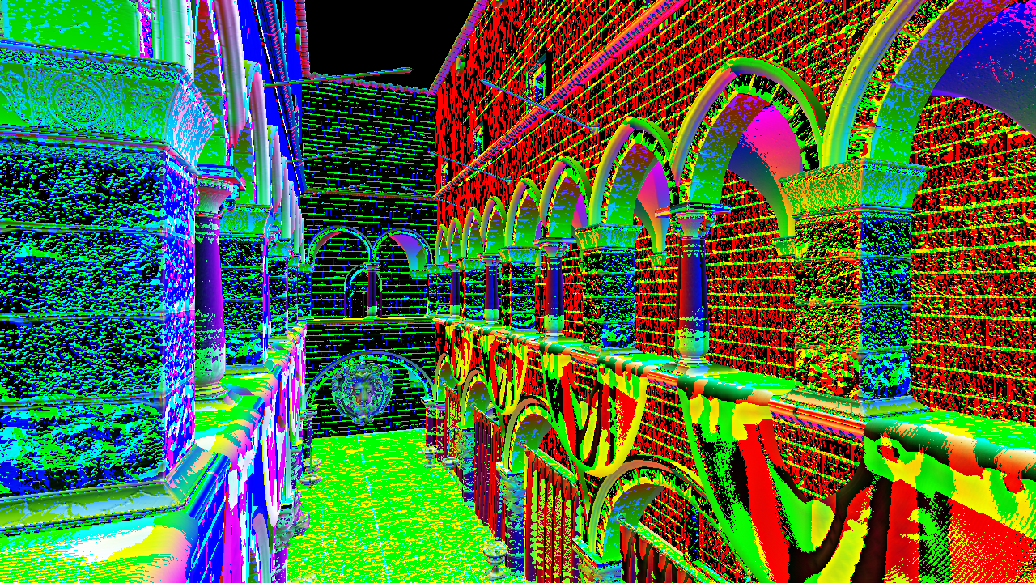
\includegraphics[width=\linewidth]{media/engine-Context2-Texture13level0.png}
		\caption*{Normales.}
	\end{subfigure}%
	\hspace{0.01\textwidth}
	\begin{subfigure}[t]{0.32\textwidth}
		\centering
		\captionsetup{justification=centering}
		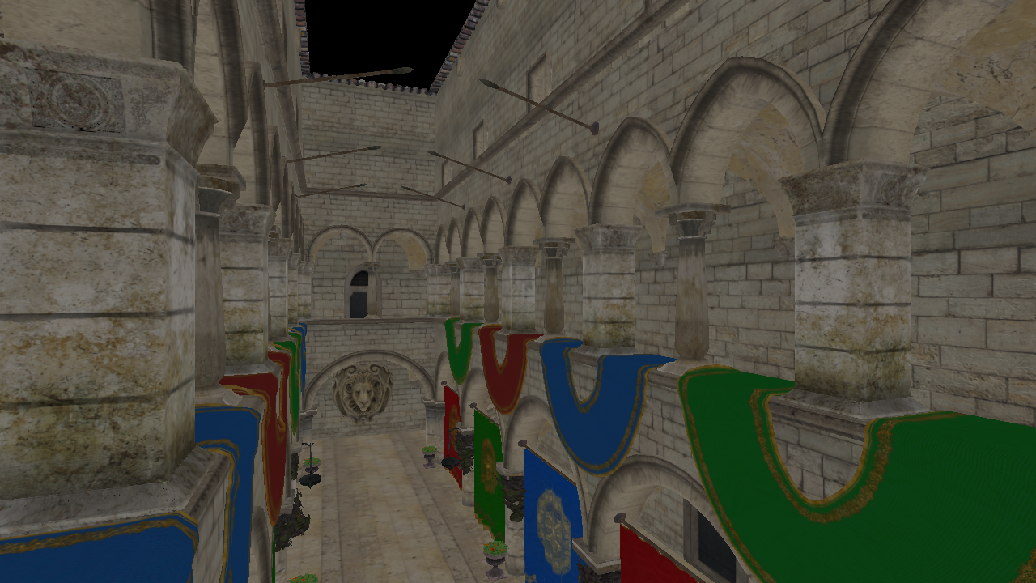
\includegraphics[width=\linewidth]{media/engine-Context2-Texture14level0.png}
		\caption*{Albedo.}
	\end{subfigure}%
	\hspace{0.01\textwidth}
	\begin{subfigure}[t]{0.32\textwidth}
		\centering
		\captionsetup{justification=centering}
		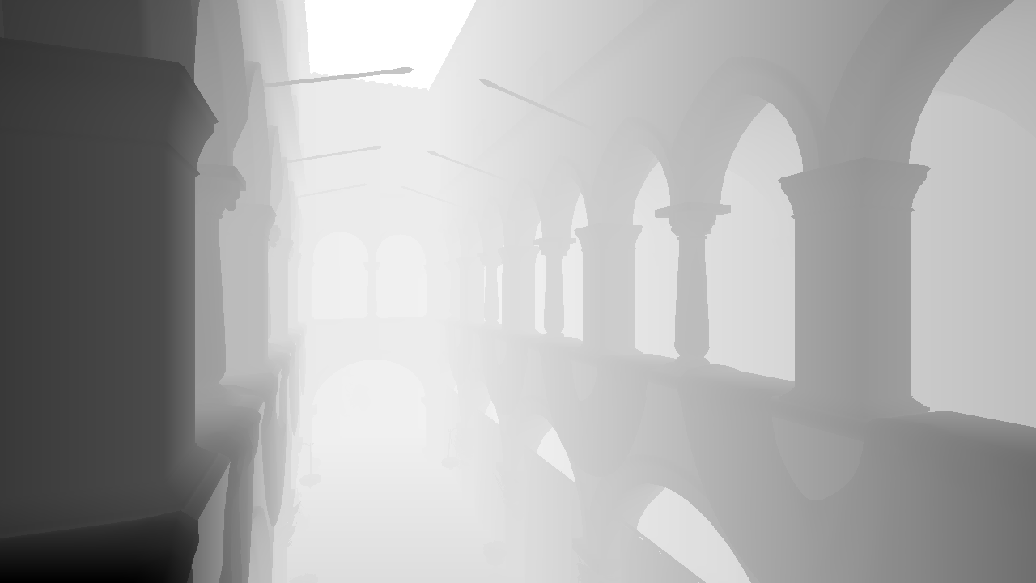
\includegraphics[width=\linewidth]{media/engine-Context2-Texture17level0.png}
		\caption*{Profundidad.}
	\end{subfigure}%
	\caption{El contenido de un buffer de geometría.}
	\label{fig:gbuffer}
\end{figure}

\subsection{Voxelización}
\label{sec:voxelization}
Un \emph{voxel} o a veces llamado píxel volumétrico representa una muestra singular o elemento volumétrico sobre un grid regular en un espacio tridimensional. Este vóxel puede contener cualquier valor definido por la aplicación o incluso múltiples valores. 

El proceso de generar superficies discretas en una representación volumétrica a través de vóxeles se le llama voxelización. En la Figura \ref{fig:rigid_grid} se ilustra este proceso.

\begin{figure}[H]
	\centering
	\begin{subfigure}{0.33\textwidth}
		\centering
		\includegraphics[width=.6\linewidth]{media/rigid01.pdf}
		\captionsetup{width=0.95\textwidth}
		\caption{Grid regular del vóxeles.}
	\end{subfigure}%\\
	\begin{subfigure}{0.33\textwidth}
		\centering
		\includegraphics[width=.6\linewidth]{media/rigid02.pdf}
		\captionsetup{width=0.95\textwidth}
		\caption{Superficie en el grid.}
	\end{subfigure}%\\
	\begin{subfigure}{0.33\textwidth}
		\centering
		\includegraphics[width=.6\linewidth]{media/rigid03.pdf}
		\captionsetup{width=.95\textwidth}
		\caption{Superficie en vóxeles.}
	\end{subfigure}%
	\caption{Representación de una superficie en vóxeles con voxelización fina.}
	\label{fig:rigid_grid}
\end{figure}

Se puede distinguir el proceso de voxelización de superficies en dos clases: voxelización fina con separabilidad factor 6 y voxelización conservativa con todos los vóxeles que tocan la superficie activos o separabilidad factor 26. En el trabajo de Huang et al. en 1998 \cite{Huang:1998:AMV:288126.288181} se describe el proceso de voxelización y terminología con mayor detalle. También existen cuatro tipos de enfoques en voxelización:

\begin{itemize}
	\label{list:voxelization_types}
	\item \textbf{Voxelización binaria:} Cada vóxel sólo almacena si hay geometría presente o no.
	\item \textbf{Voxelización multi-valor:} Cada vóxel puede almacenar múltiples valores de data arbitraria como opacidad, normal, etc.
	\item \textbf{Voxelización de contorno:} Sólo se voxeliza la superficie o contorno de los objetos.
	\item \textbf{Voxelización sólida:} Además de la superficie también se voxeliza el interior del objeto.
\end{itemize}

\section{Iluminación Global en Tiempo Real.}
\label{sec:interactive_gi_takes}
En esta sección se examinan algunos algoritmos para el cálculo de iluminación global en tiempos interactivos o \emph{real-time}. Iluminación indirecta con trazado de conos y vóxeles es revisada con detalle ya que esta técnica es de particular interés para este trabajo.

\subsection{Luces Puntuales Virtuales}
Una variedad de algoritmos para el cálculo de iluminación global se inspiran o hacen uso del concepto de \ac{VPL}. Este trabajo fue presentado por Keller en 1997 \cite{Keller:1997}.

\begin{figure}[H]
	\centering
	\begin{subfigure}[h]{0.35\textwidth}
		\centering
		\captionsetup{justification=centering}
		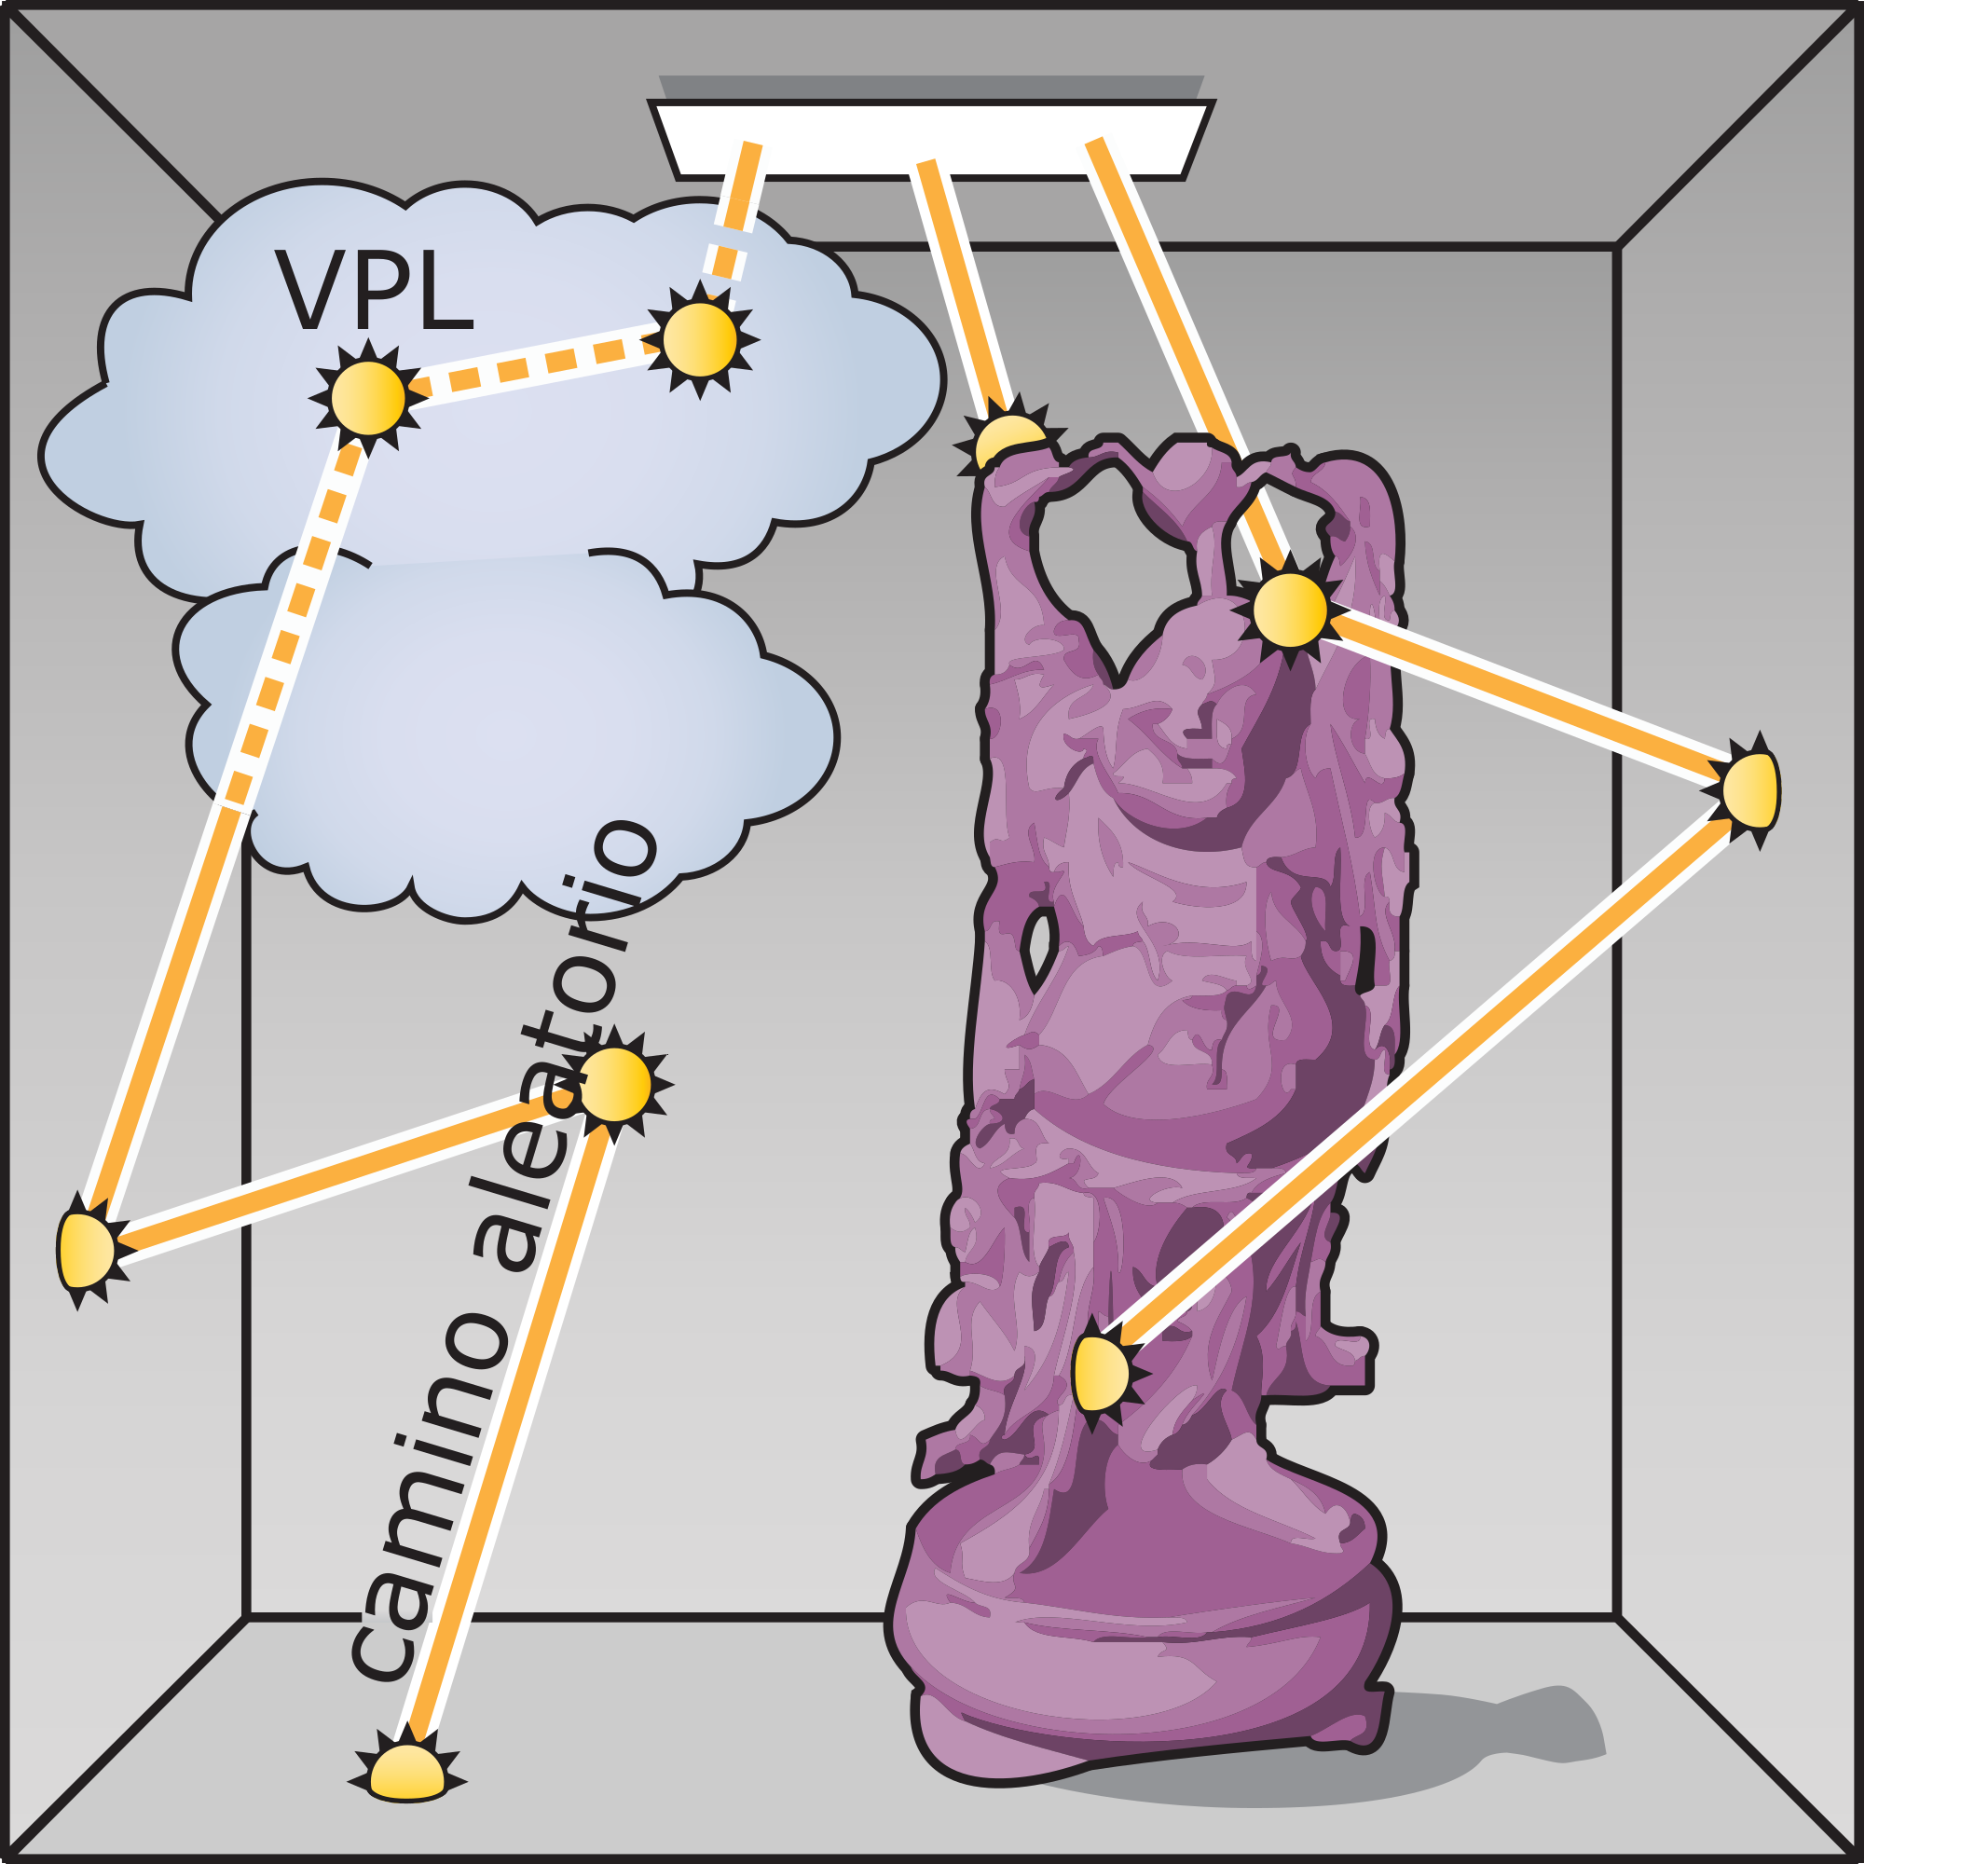
\includegraphics[width=\linewidth]{media/vpl1.png}
		\caption*{Generación de luces virtuales puntuales}
	\end{subfigure}
	\hspace{0.1\textwidth}
	\begin{subfigure}[h]{0.35\textwidth}
		\centering
		\captionsetup{justification=centering}
		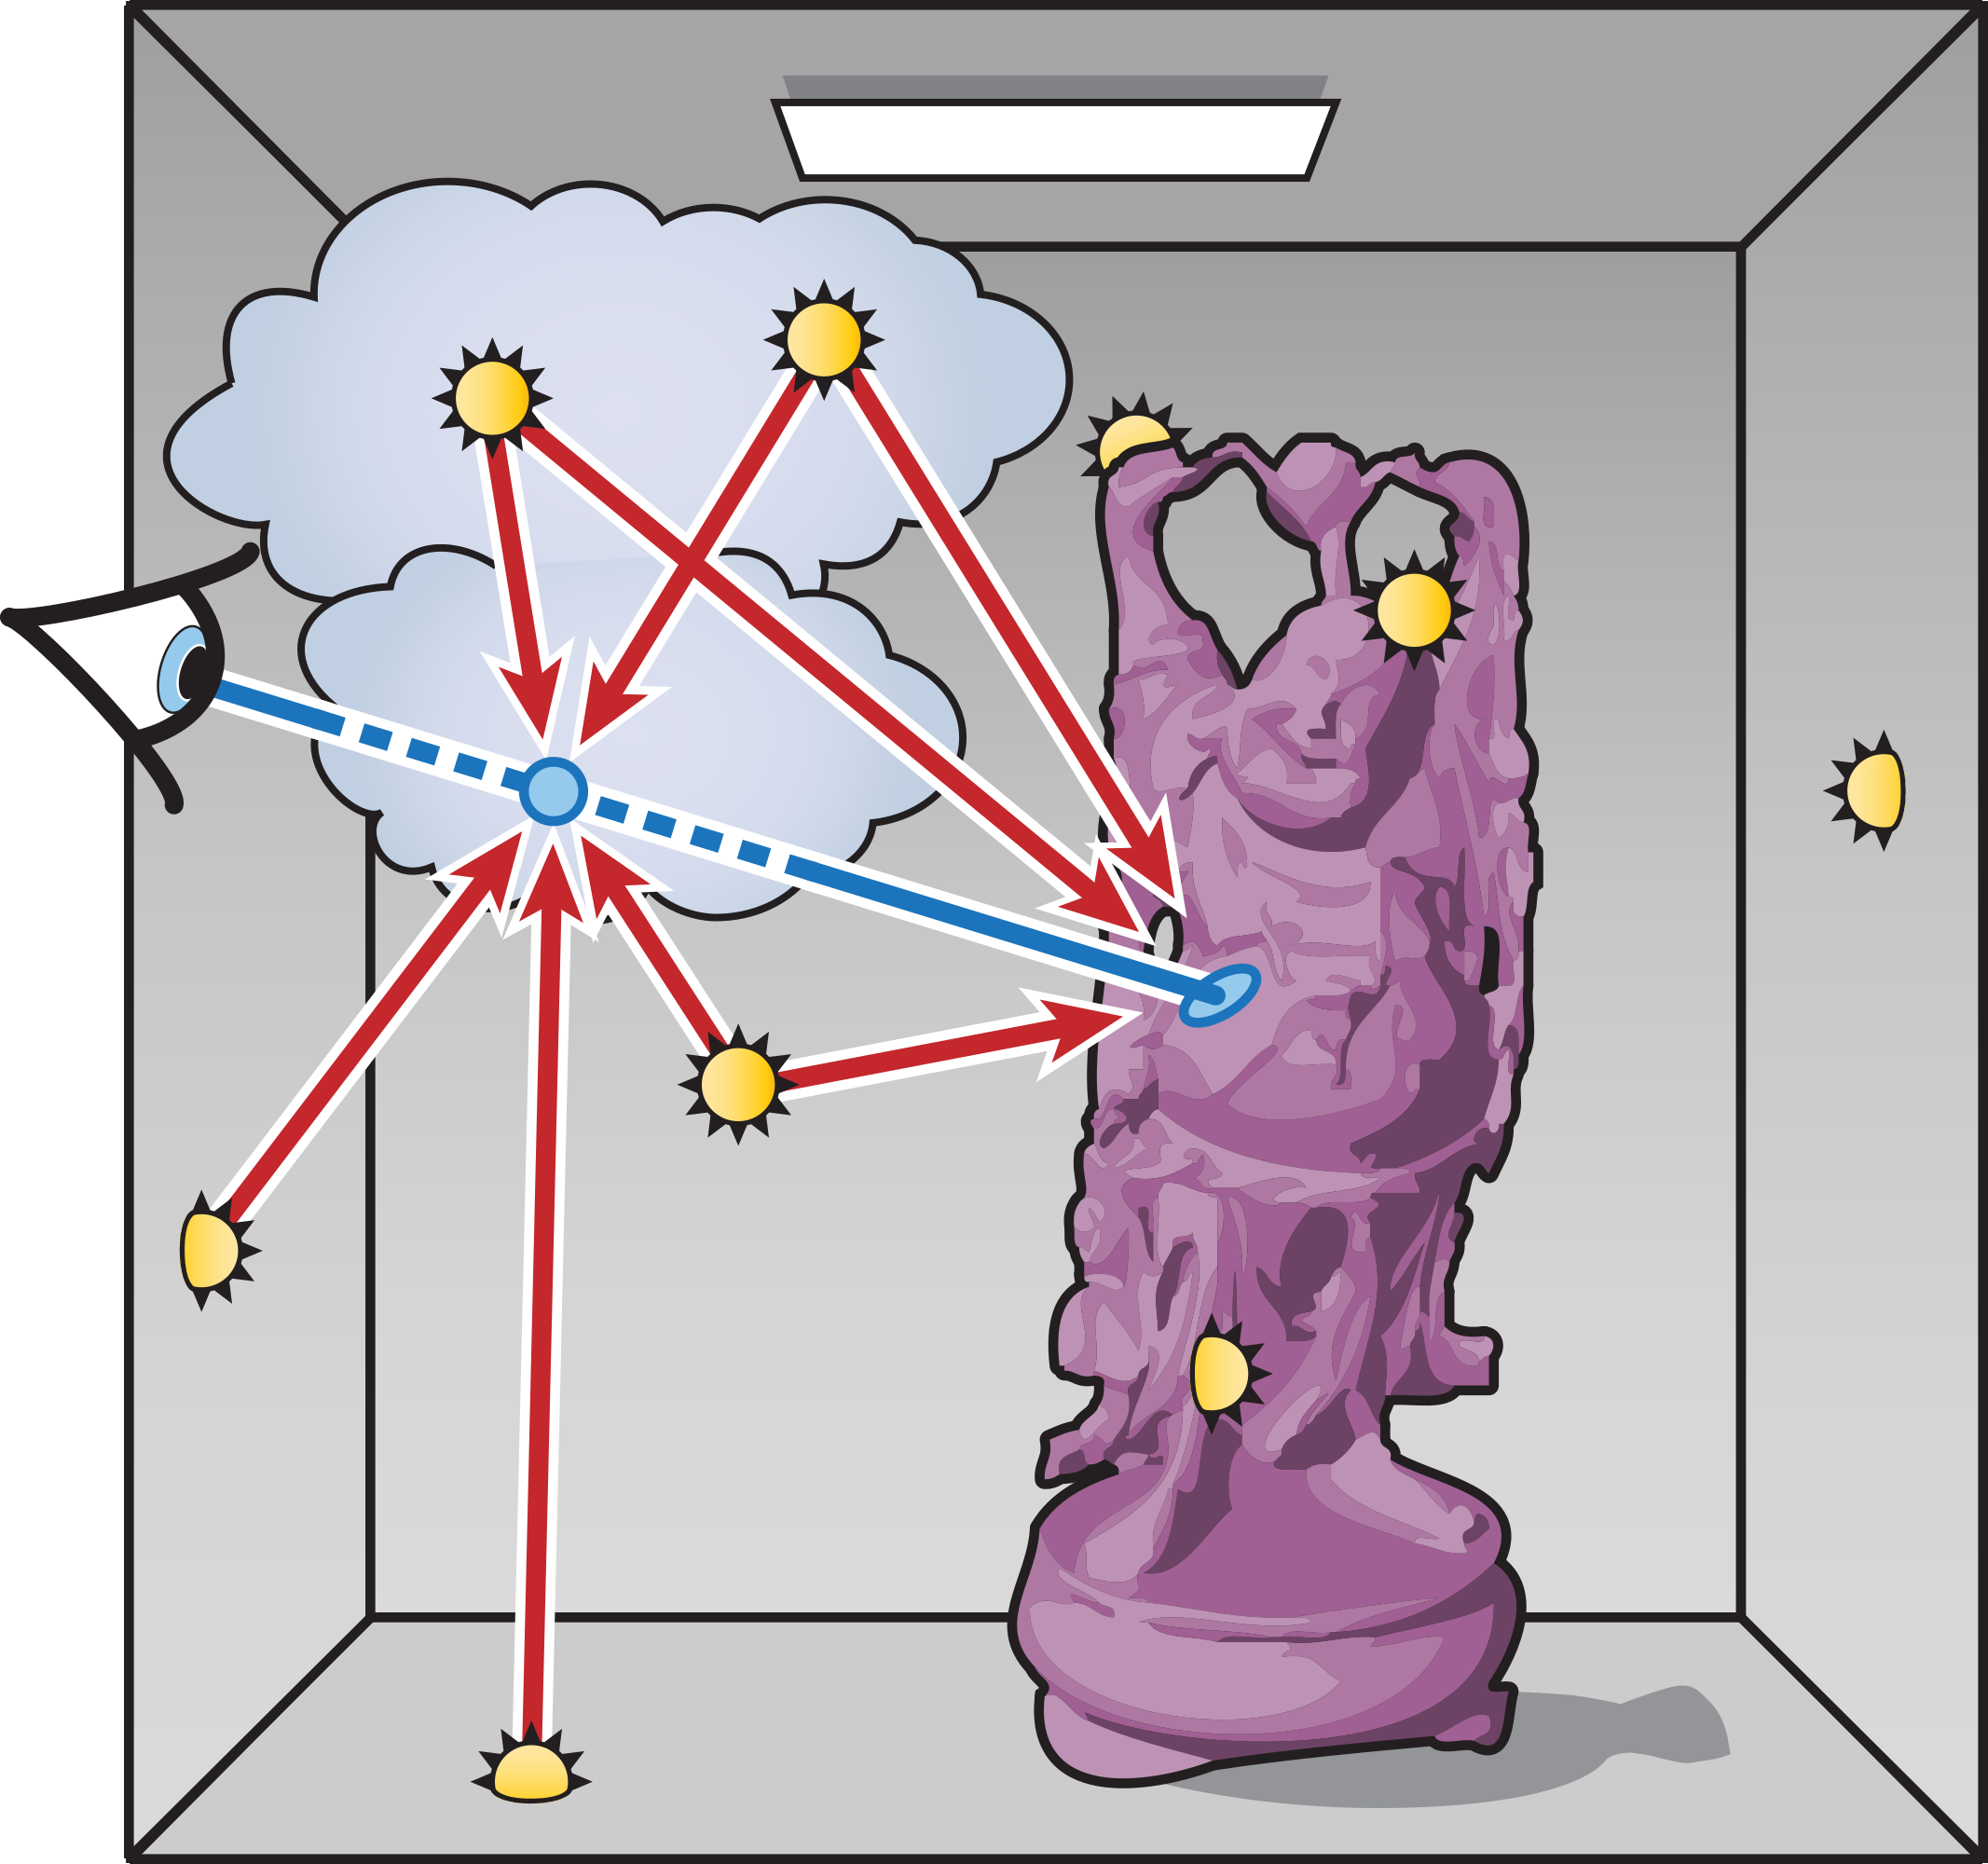
\includegraphics[width=\linewidth]{media/vpl2.png}
		\caption*{Aproximación de iluminación acumulada sobre un punto.}
	\end{subfigure}
	\caption{Pasos del algoritmo \ac{VPL} para la aproximación de iluminación indirecta \cite{Dachsbacher2014ManyLights}.}
	\label{fig:vpl_passes}
\end{figure}


En este algoritmo se aproxima la radiancia reflectada en escena utilizando un conjunto de luces virtuales. La radiancia que llega a un punto $x$ es aproximada por la radiancia que proviene de las luces virtuales. Pruebas de visibilidad para cada una de estas luces son realizadas utilizando técnicas de sombreado estándar y la radiancia proveniente de cada una de estas es almacenada en un buffer de acumulación. En la Figura \ref{fig:vpl_passes} se ilustra este algoritmo.
Las luces virtuales son generadas a partir de partículas lanzadas por las fuentes de luz principales utilizando la secuencia de Halton para el muestreo. En un principio, un número $n$ de partículas son generadas, como no toda la radiancia es absorbida algunas de estas partículas son reflejadas. Luego del primer rebote, uno número $p'n$ de partículas son reflejadas. Luego de $j-1$ reflexiones $p'^j$ son reflejadas. El número $p'$ es descrito por la siguiente ecuación:
\begin{equation}
    p' = \frac{\sum_{k=1}^{K} p_{d,k}|A_{k}|}{\sum_{k=1}^{K}|A_{k}|}
    \label{eq:reflected_vpls}
\end{equation} donde la escena es compuesta por $K$ elementos de superficie $A_{k}$ con una reflectividad promedio de $p_{d,k}$.

\subsection{Mapas de Sombras Reflexivo}
Otra técnica utilizada en varios algoritmos de iluminación global es \ac{RSM} o \emph{reflective shadow maps}. La técnica de \ac{RSM} fue presentada por Dachsbacher y otros en 2005 \cite{Dachsbacher:2005}.  Esta técnica está inspirada en mapeado de sombras, como fue explicado anteriormente en la sección \ref{subsec:shadowmapping}, se utiliza proyección desde la fuente de luz para determinar el primer rebote de luz. Al renderizar la escena desde el punto de vista de la fuente de luz, se entiende que todos los fragmentos en el mapa de sombras son los únicos fragmentos involucrados en el primer rebote de luz. En \ac{RSM} cada uno de los píxeles en el mapa de sombras es considerado una fuente de luz. Por cada píxel $p$ además de la profundidad $d_{p}$, se necesita almacenar posición $x_{p}$, normal $n_{p}$, y el flujo de radiancia reflectada $\Theta_{p}$ (ver Figura \ref{fig:rsm_fbo}).

\begin{figure}[H]
	\centering
	\begin{subfigure}[t]{.24\linewidth}
		\centering
		\captionsetup{justification=centering}
		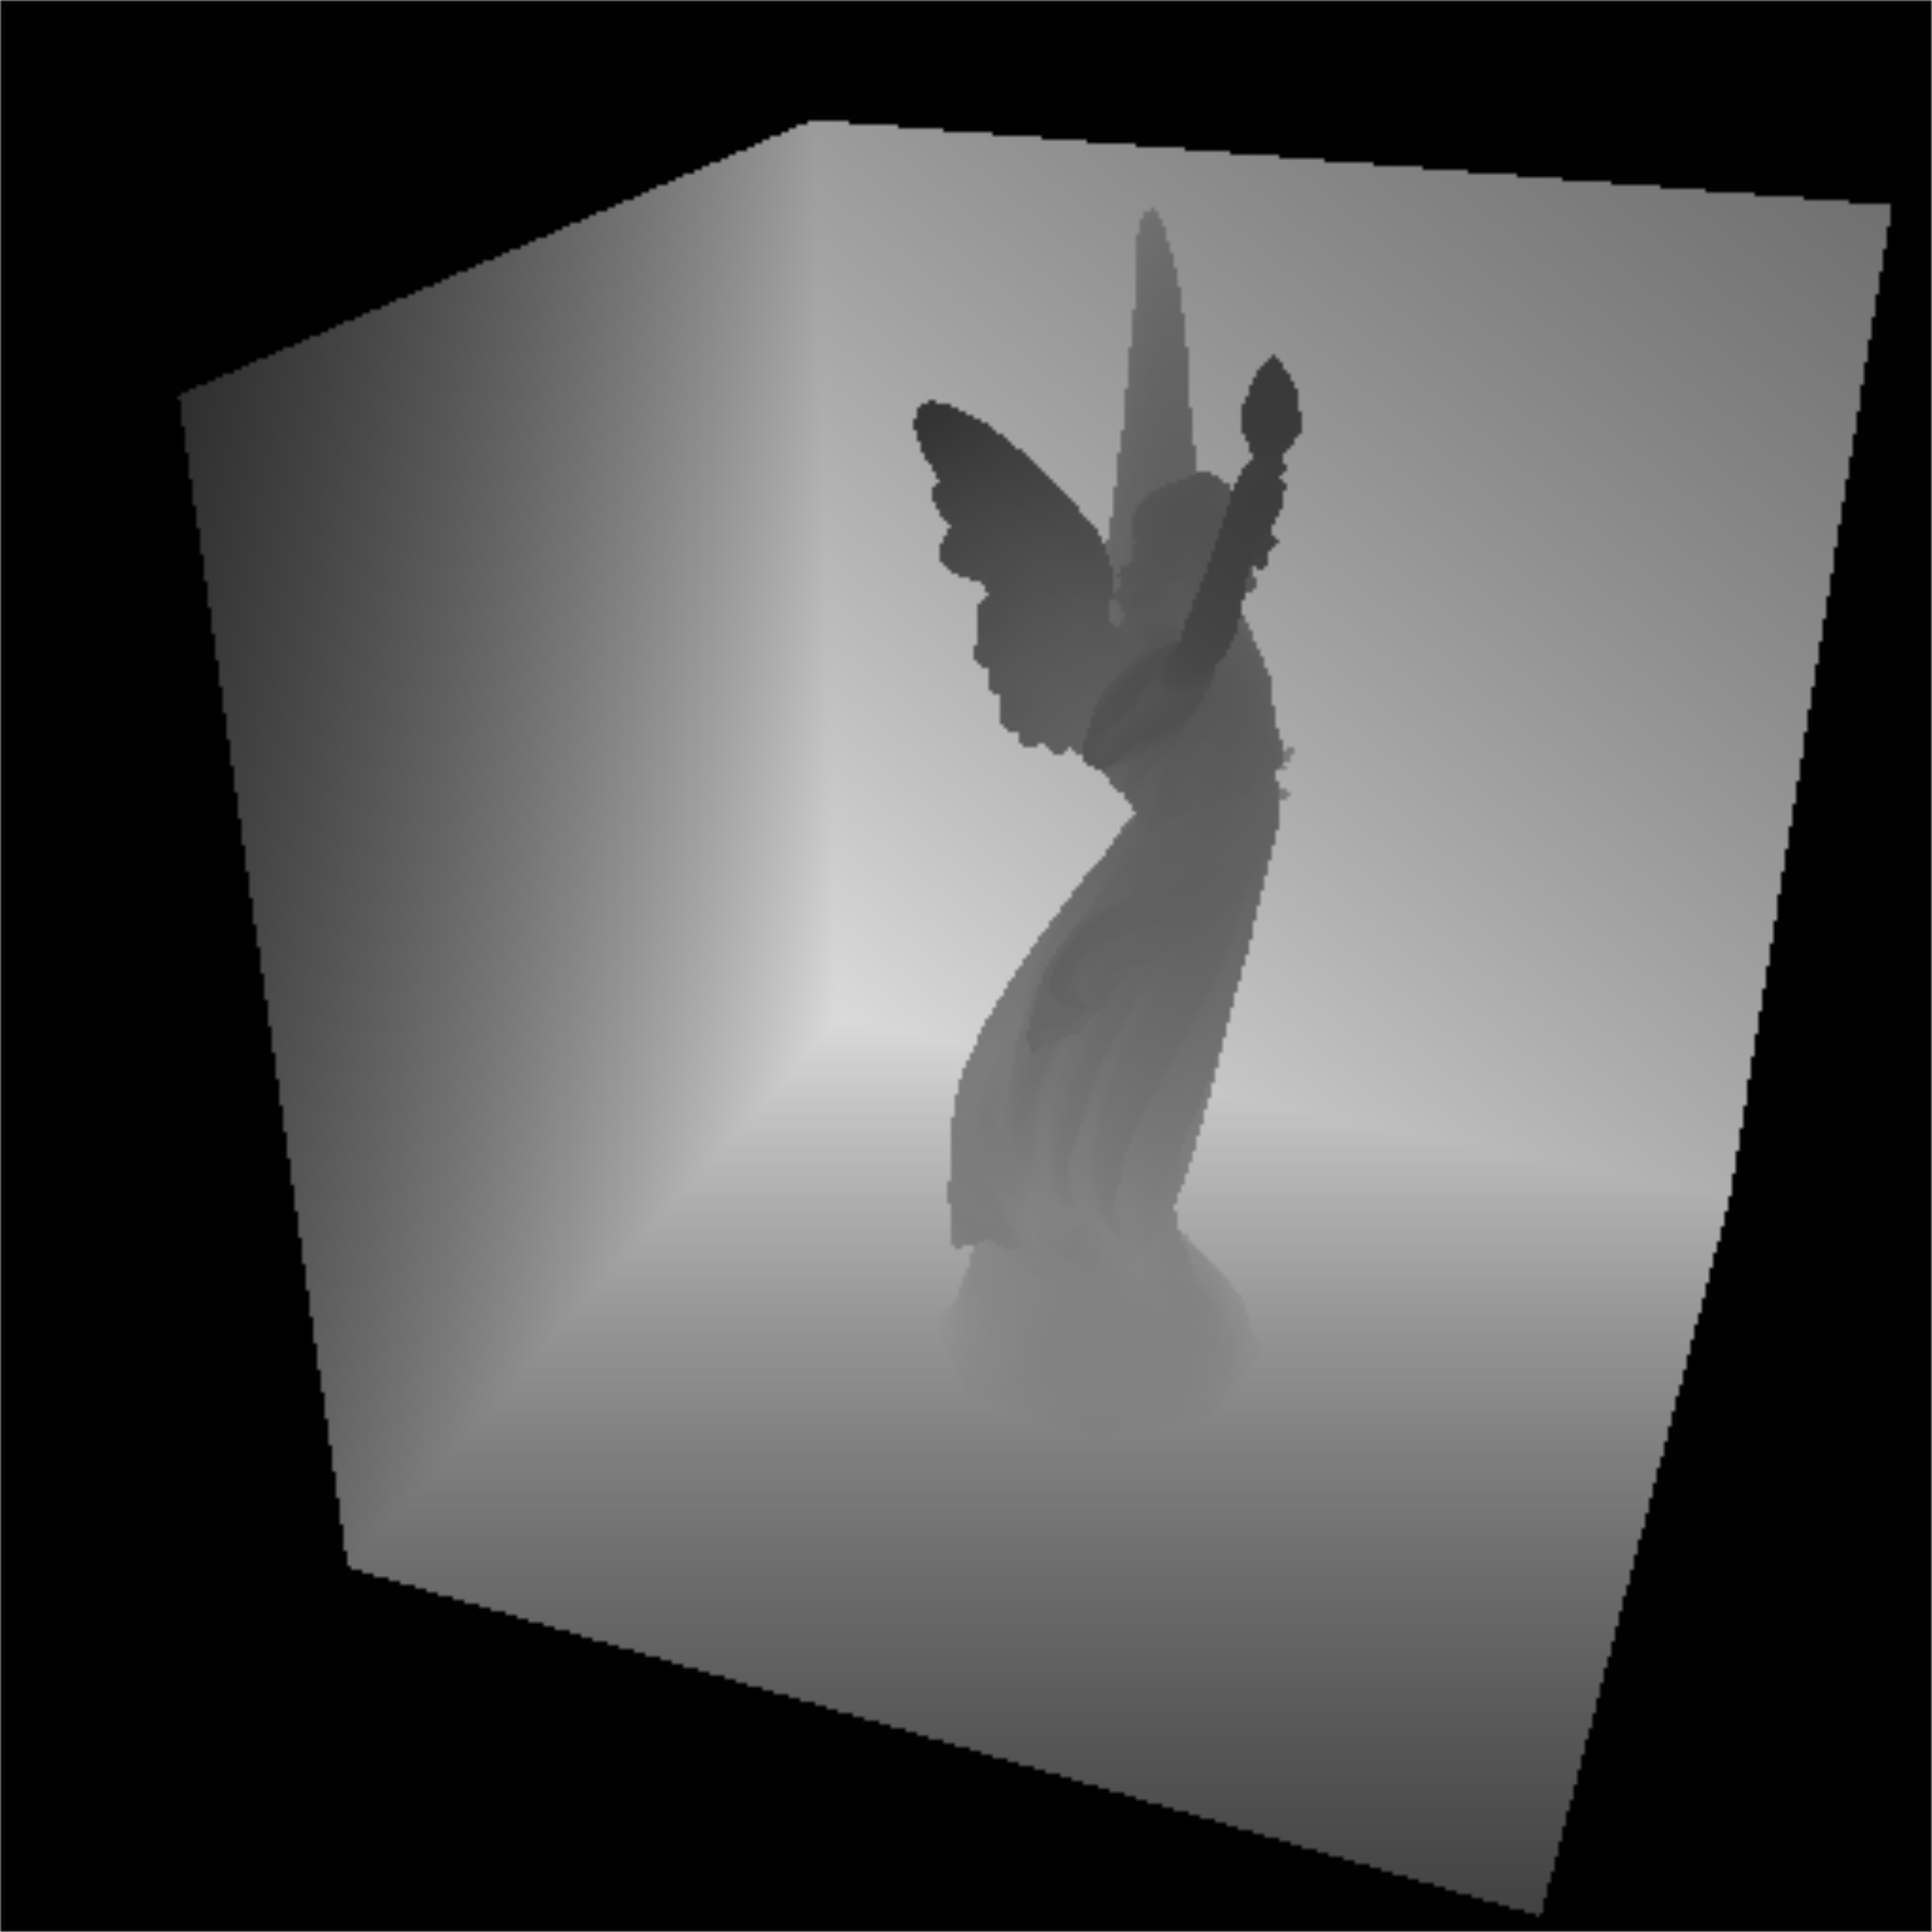
\includegraphics[width=\linewidth]{media/rsmd.png}
		\caption*{Profundidad.}
	\end{subfigure}
	\begin{subfigure}[t]{.24\linewidth}
		\centering
		\captionsetup{justification=centering}
		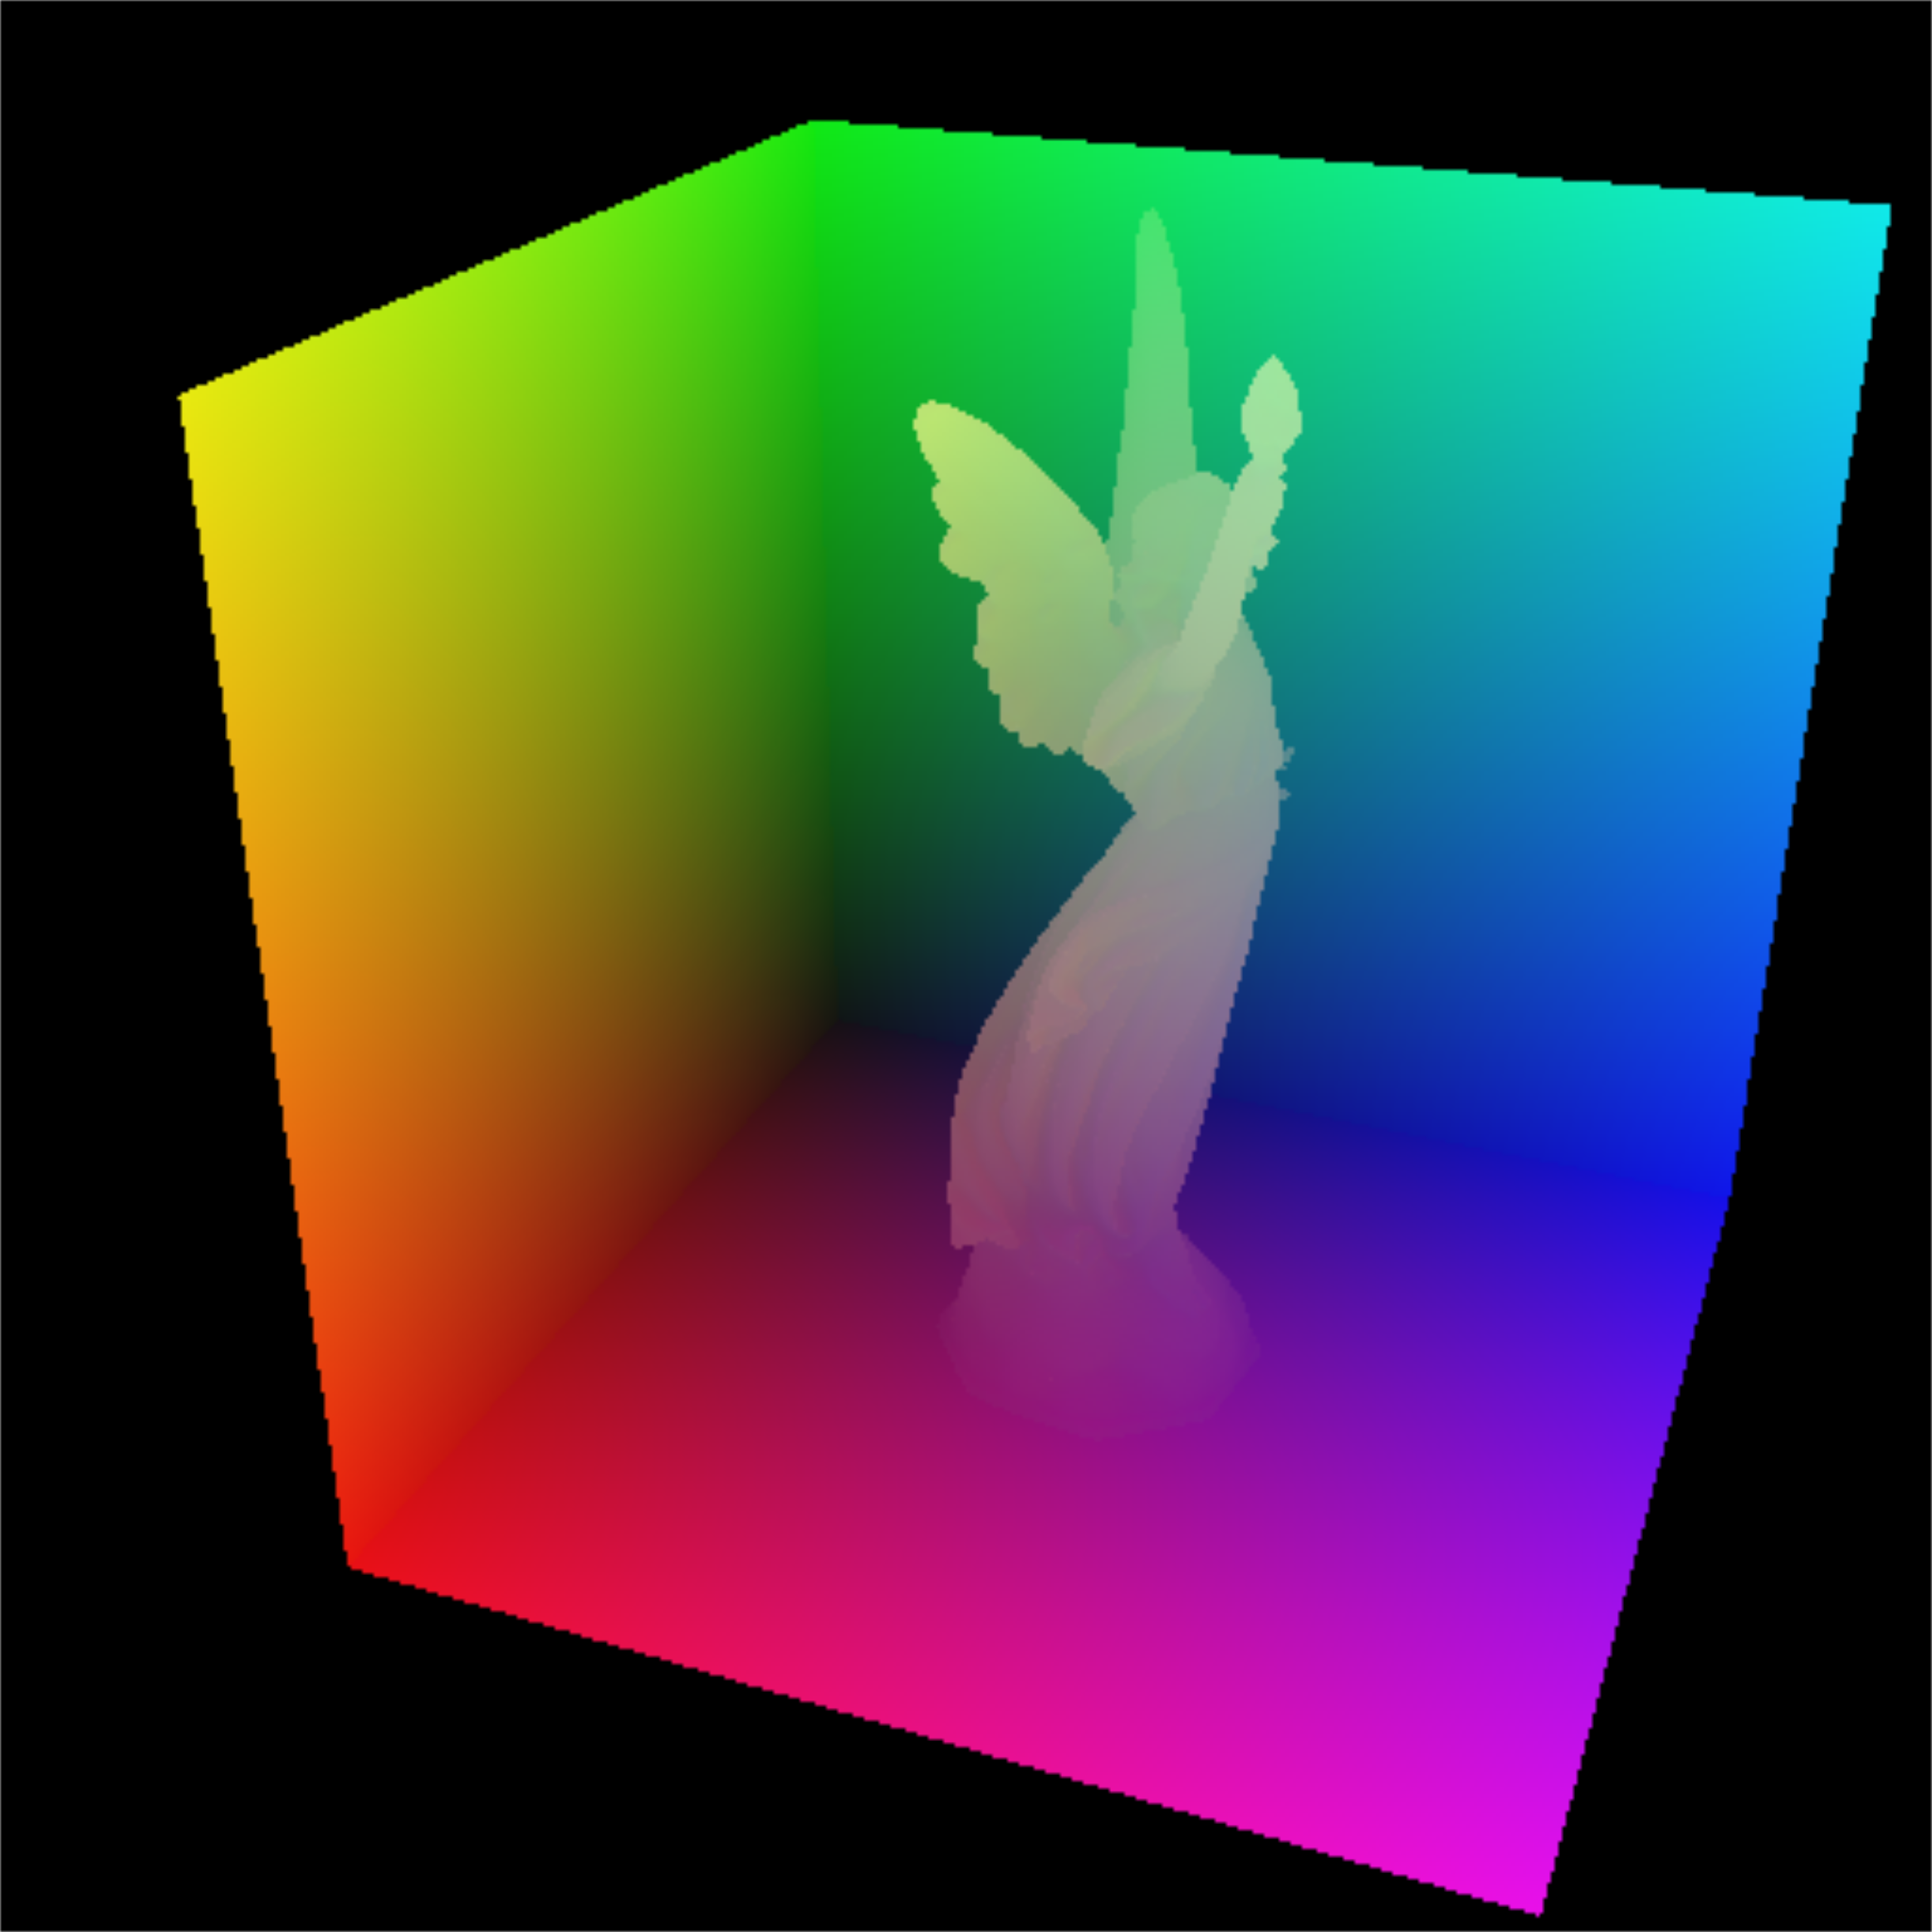
\includegraphics[width=\linewidth]{media/rsmp.png}
		\caption*{Posición.}
	\end{subfigure}
	\begin{subfigure}[t]{.24\linewidth}
		\centering
		\captionsetup{justification=centering}
		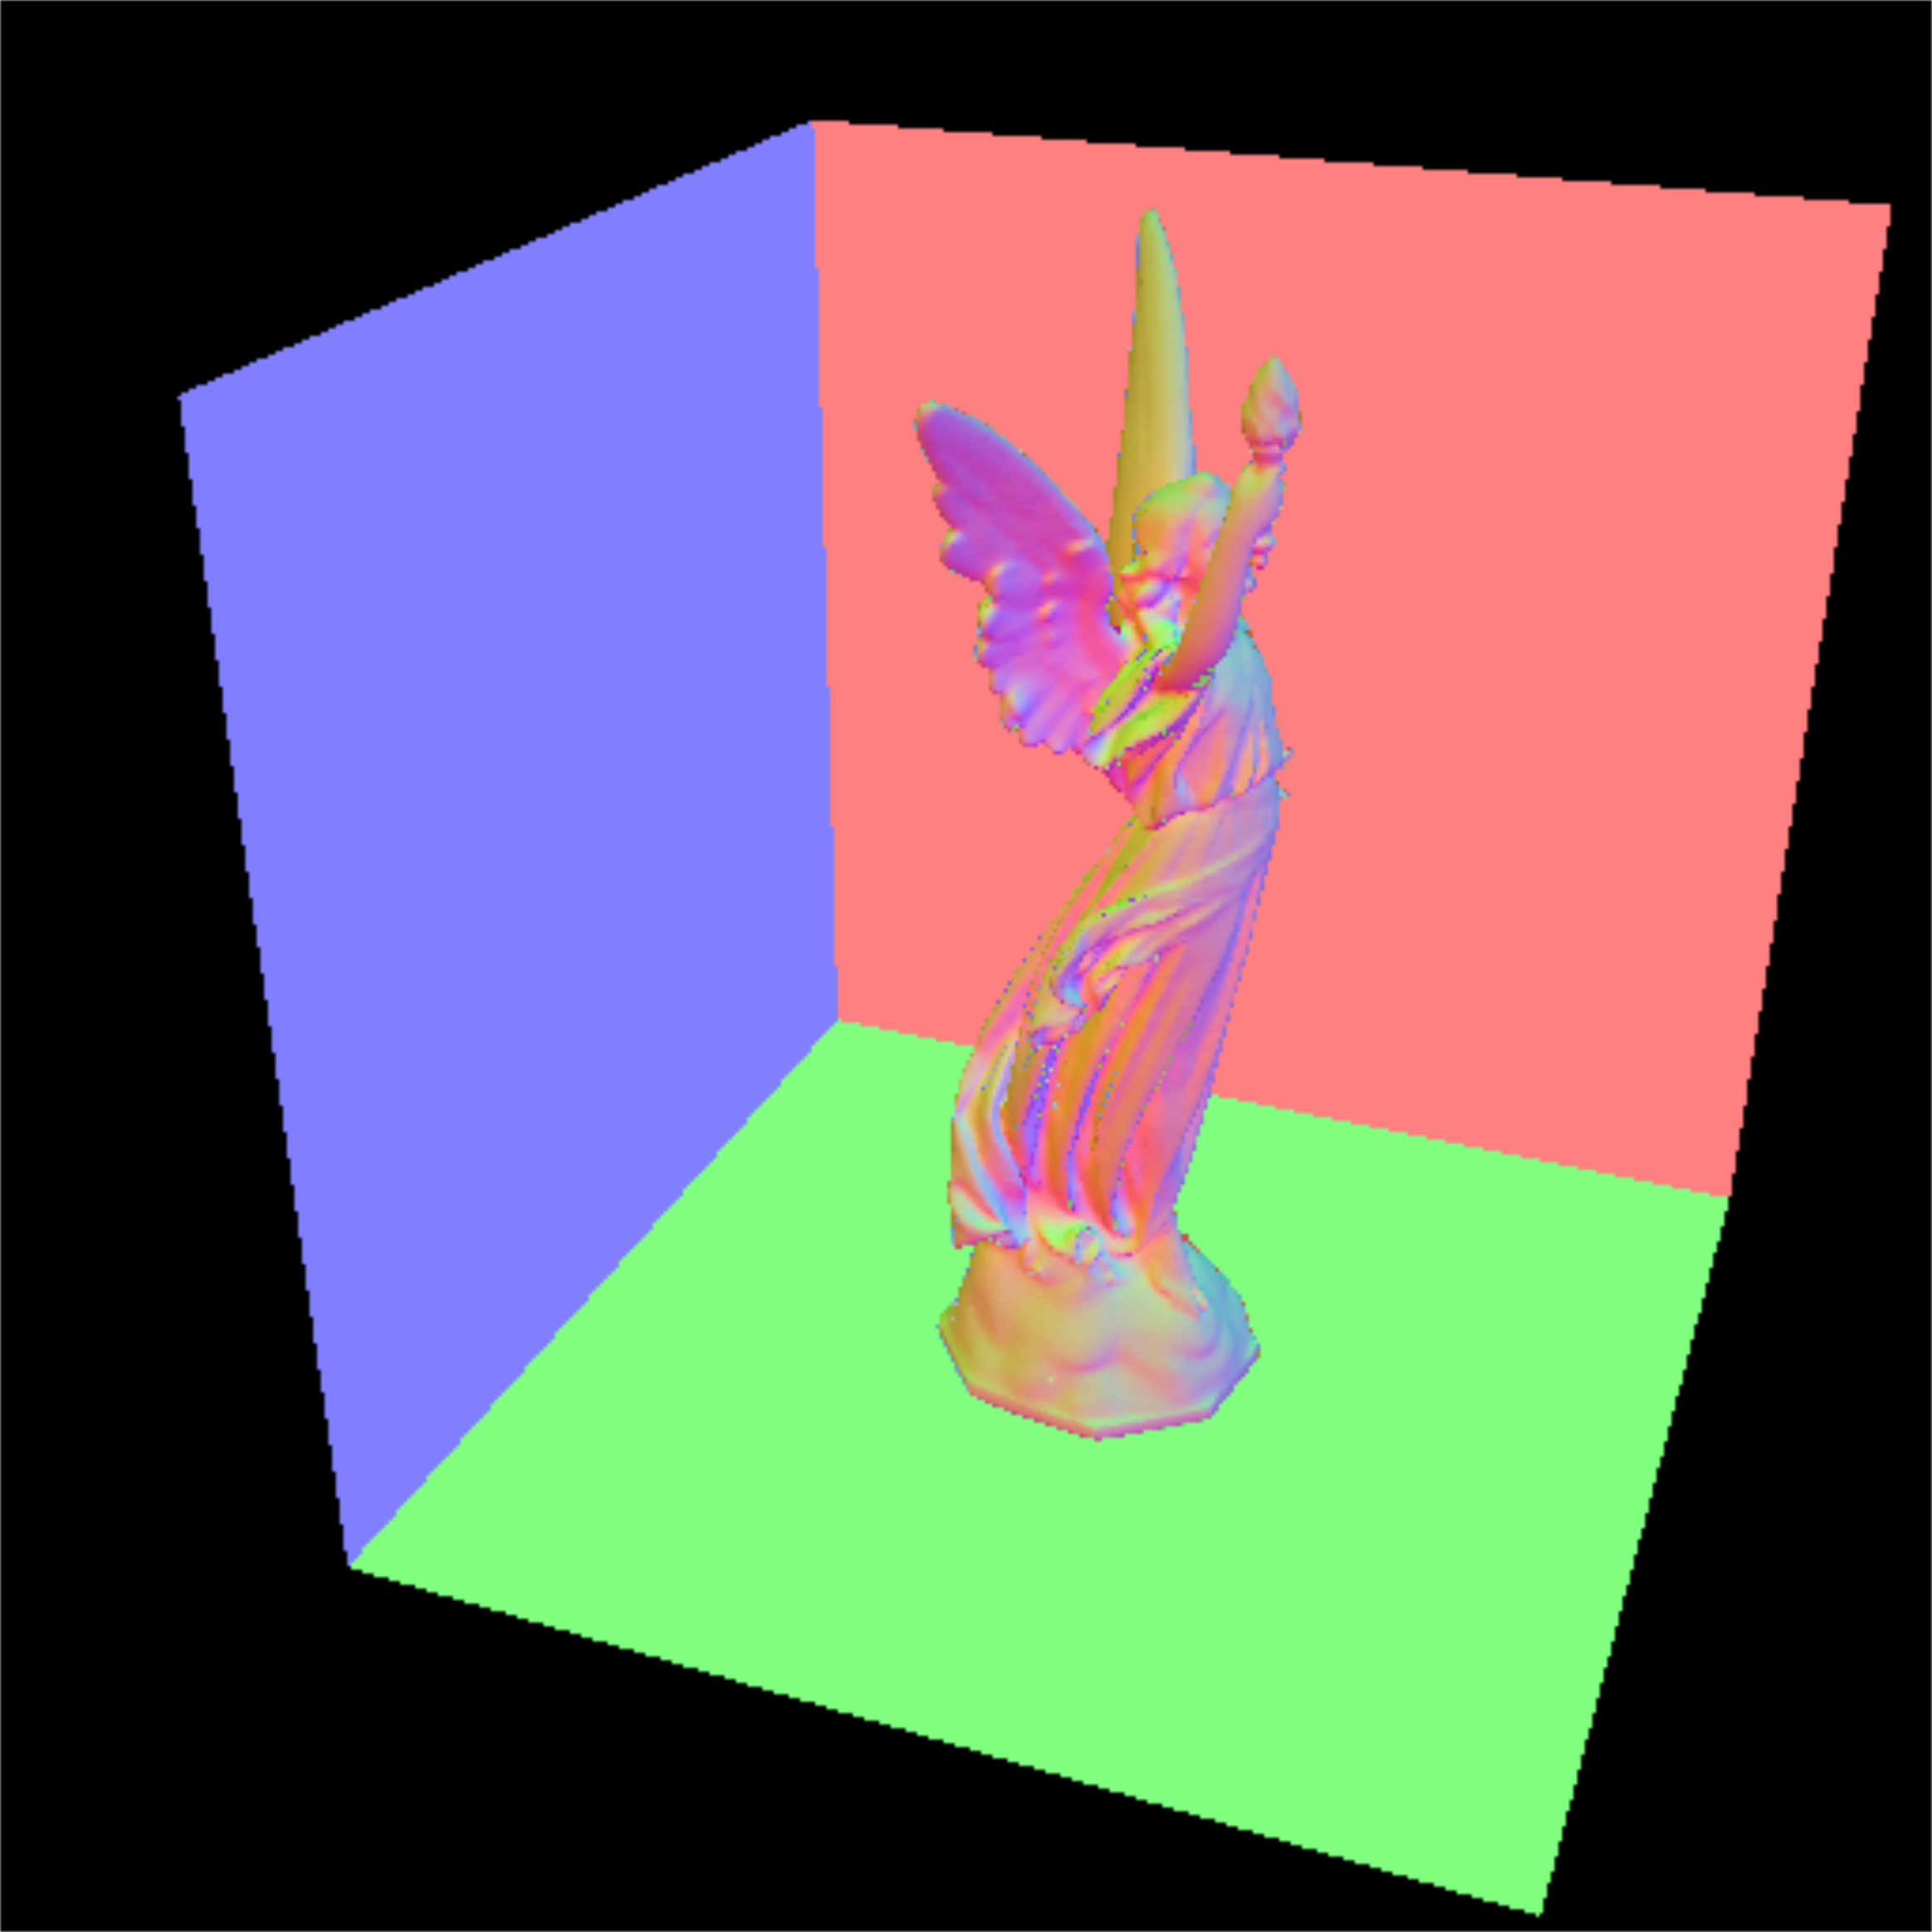
\includegraphics[width=\linewidth]{media/rsmn.png}
		\caption*{Normal.}
	\end{subfigure}
	\begin{subfigure}[t]{.24\linewidth}
		\centering
		\captionsetup{justification=centering}
		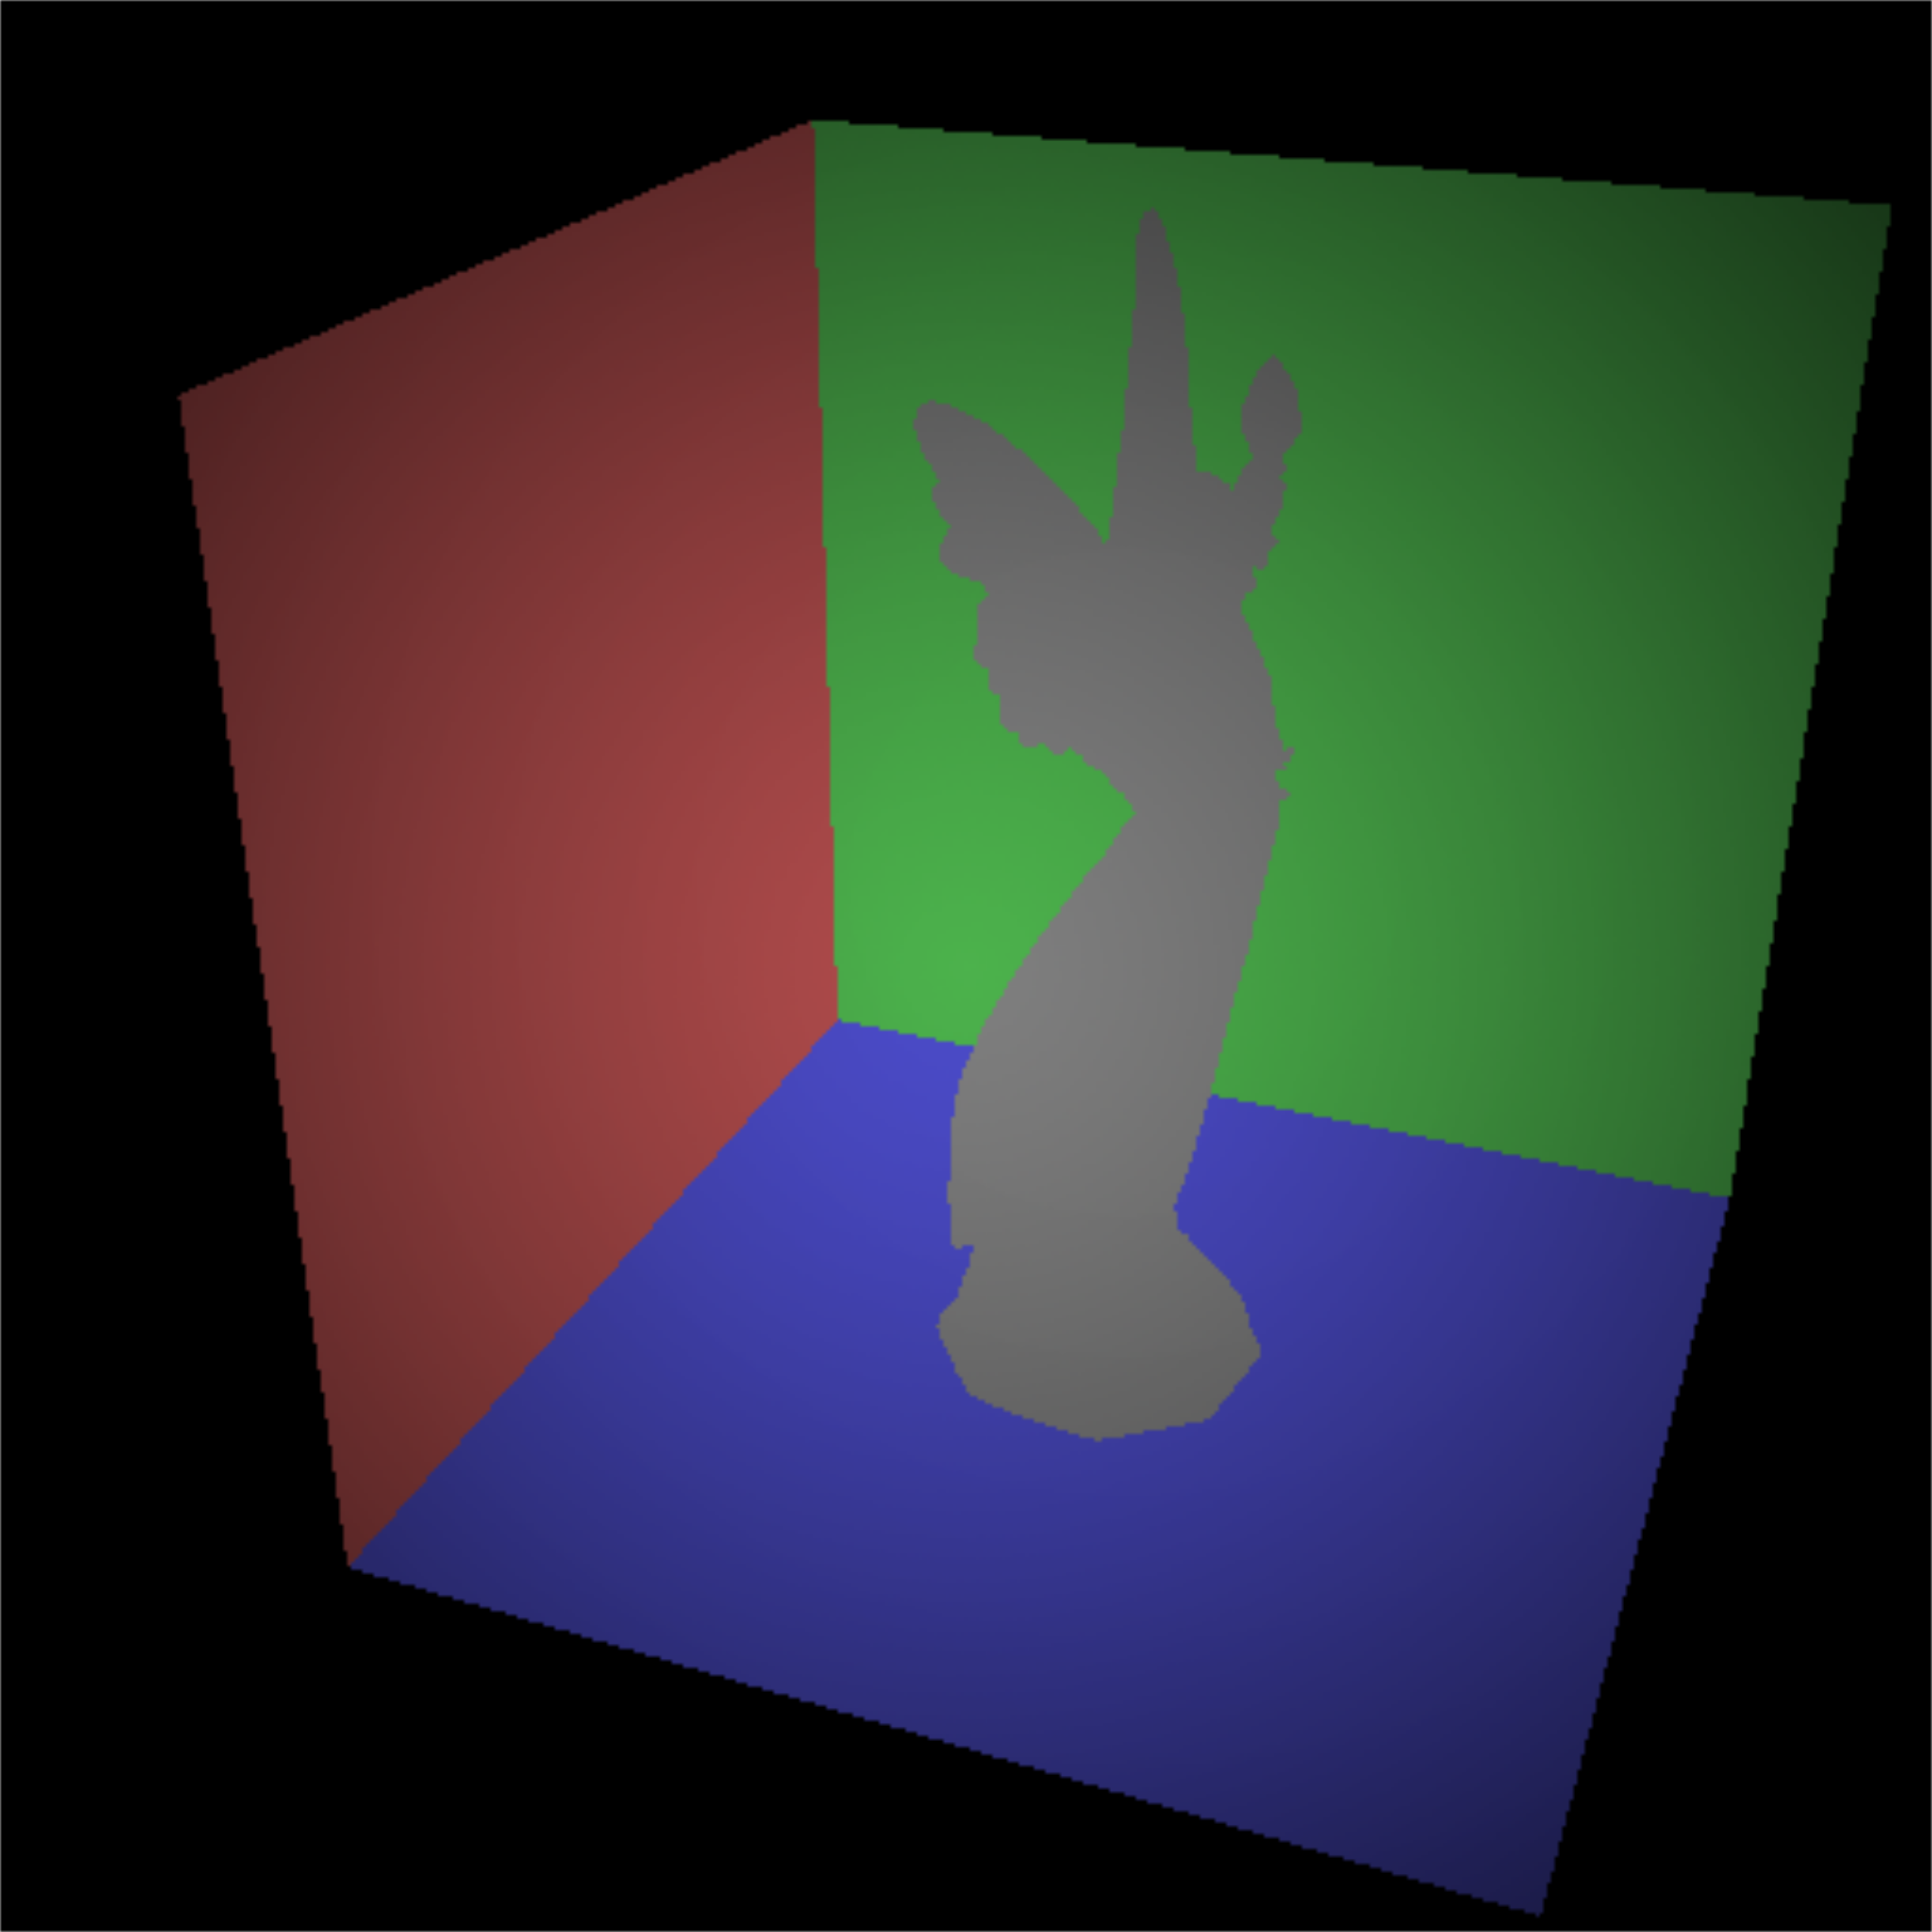
\includegraphics[width=\linewidth]{media/rsmf.png}
		\caption*{Flujo de radiancia.}
	\end{subfigure}
	\caption{Mapas utilizados por \ac{RSM} \cite{Dachsbacher:2005}.}
	\label{fig:rsm_fbo}
\end{figure}

Si se asume que todas las superficies son reflectores difusos, la intensidad de la radiancia emitida en una dirección $\omega$ desde un píxel del \ac{RSM} es descrita por la siguiente ecuación:

\begin{equation}
    I_{p}(\omega) = \Theta_{p}max(0, n_{p} \cdot {w})
    \label{eq:rsm_radiance}
\end{equation}

La iluminación indirecta de un punto se calcula sumando todas las intensidades de todos los píxeles (considerados ahora como luces) en el \ac{RSM} visibles. Calcular esto es costoso, por tanto en vez sumar todos los píxeles visibles al punto se toma cierta cantidad de muestras del \ac{RSM}. La posición del punto iluminado $x_{p}$ es proyectado sobre el \ac{RSM} y las muestras son seleccionadas alrededor de esta posición proyectada. La densidad de las muestras decrece con la distancia cuadrada de la posición proyectada al punto iluminado. Esta técnica asume que dos superficies cercanas proyectadas al \ac{RSM} también son cercanas en el \ac{RSM} y que la muestra es directamente visible desde la superficie iluminada.

\subsection{Volúmenes de Propagación de Luz en Cascada}
\label{sub:clpv}
\Ac{CLPV} o \emph{Cascaded Light Propagation Volumes} presentando por Kaplanyan et al. en 2010 \cite{Kaplanyan:2010} es un algoritmo para el cálculo de iluminación indirecta difusa en tiempo real. En la Figura \ref{fig:lvp_results} se observan los resultados de esta técnica.

\begin{figure}[H]
	\centering
	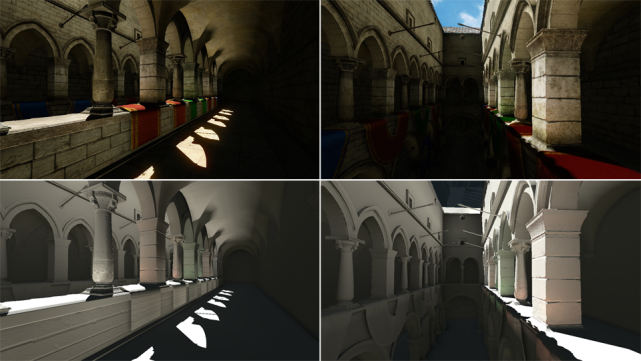
\includegraphics[width=0.85\linewidth]{media/lpvresult.png}
	\caption{Iluminación global para la escena \emph{Sponza} utilizando volúmenes de propagación de luz \cite{Kaplanyan:2010}.}
	\label{fig:lvp_results}
\end{figure}

\begin{wrapfigure}[11]{l}{0.3\linewidth}
	\centering
	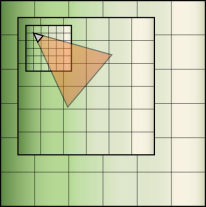
\includegraphics[width=0.90\linewidth]{media/g4957.png}
	\caption{Cuadrículas de \\ propagación anidadas, las cuadrículas se solapan.}
	\label{fig:nested_lpv}
\end{wrapfigure}
\noindent Este método simula el transporte de luz utilizando técnicas similares en algoritmos para simulación de fluidos basados en cuadrículas tridimensionales \cite{Crane07}. La intensidad de luz es almacenada en una cuadrícula y de forma iterativa cada celda transfiere la intensidad de la luz a sus vecinos. Esta cuadrícula es llamada \ac{LPV}. La luz puede ser bloqueada por la geometría de la escena, la cual es obtenida de otra cuadrícula llamada \ac{GV}. Para mejorar el rendimiento del algoritmo y reducir el consumo de memoria se utiliza un conjunto de cuadrículas anidadas (ver Figura \ref{fig:nested_lpv}). Para los objetos cercanos al observador la iluminación indirecta es calculada utilizando una cuadrícula mucho más fina.

Primero por cada fuente de luz, es necesario renderizar un \ac{RSM}. Cada téxel del \ac{RSM} es considerado una \ac{VPL}. La intensidad del \ac{VPL} es acumulada y almacenada como un harmónico esférico dentro de las celdas de la cuadrícula.

Para una correcta propagación de la luz el algoritmo necesita conocer la geometría de la escena. Por esto de la misma manera en la que se almacena la intensidad de la luz también se almacena una representación de la escena en una cuadrícula. Esta representación es guardada sobre el \ac{GV}. Esta cuadrícula es trasladada por la mitad del tamaño de una celda con respecto al \ac{LPV}, esto asegura que el centro de todas las celdas del \ac{GV} queden en las esquinas del \ac{LPV}. Para conocer segmentos de geometría se utiliza un \ac{GBuffer} y las fuentes de luz de los \ac{RSM}s.


\begin{figure}[H]
	\centering
	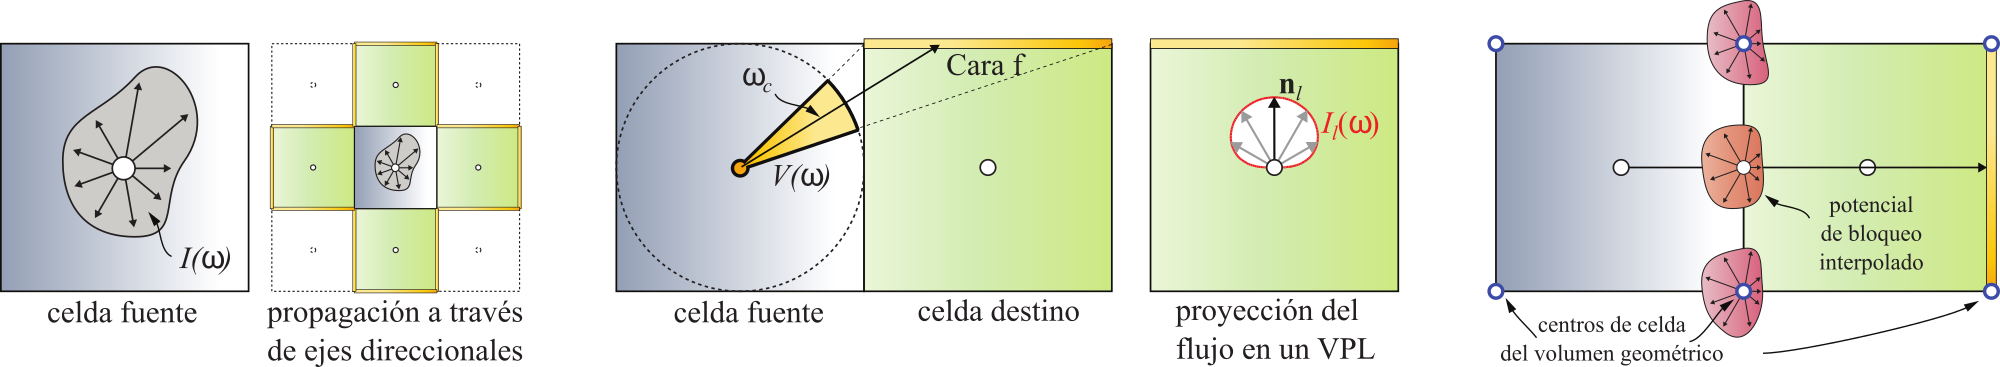
\includegraphics[width=\linewidth]{media/lpv_explain.png}
	\caption{Izquierda: Cada celda del \ac{LPV} almacena la intensidad de luz que es propagada desde la celda fuente. Centro: El flujo es calculado sobre cada cara de la celda destino para preservar información direccional. Derecha: Oclusión borrosa o \emph{fuzzy} almacenando una representación volumétrica de la escena \cite{Kaplanyan:2010}.}
	\label{fig:lpv_explain}
\end{figure}

La propagación de luz se realiza de forma iterativa. La intensidad de luz en cada iteración es propagada a 6 vecinos por celda según el eje direccional principal. Primero por cada celda adyacente el flujo de radiancia incidente por cada una de las celdas es calculado. Luego el flujo incidente de cada celda es transformado en emitancia radiante. Esto se logra creando \ac{VPL}s, cada una de estas luces virtuales son colocadas sobre una de las caras de la celda y emiten un flujo radiancia similar el flujo de radiancia de la celda. Estas \ac{VPL} son acumuladas dentro del \ac{LPV} de nuevo y almacenadas como esféricos harmónicos utilizando el mismo proceso de inyección del primer paso. En la Figura \ref{fig:lpv_explain} se describen los pasos de este algoritmo. 

\subsection{Iluminación Indirecta con Trazado de Conos y Vóxeles}
\label{sub:voxel_cone_tracing_orig}
Este algoritmo es presentado por Crassin et al. en 2011 \cite{CNSGE11b} para el cálculo de iluminación indirecta utilizando trazado de conos contra vóxeles o \emph{Indirect Illumination Using Voxel Cone Tracing}. En la Figura \ref{fig:givoxels_sponzanew1} se observan los resultados de este algoritmo. En esta técnica se utiliza una estructura de árbol disperso o \emph{sparse} para almacenar ya filtrados los valores necesarios para el cálculo de iluminación indirecta en vóxeles. Este árbol es una representación tridimensional de la escena por tanto cada nodo tiene ocho hijos que representan las ocho particiones de un cubo en partes más pequeñas de forma uniforme. Esta clase de estructuras son llamadas \emph{octrees}. La estructura dispersa requiere menor consumo de memoria ya que solo los vóxeles necesarios son almacenados.

\begin{figure}[H]
	\centering
	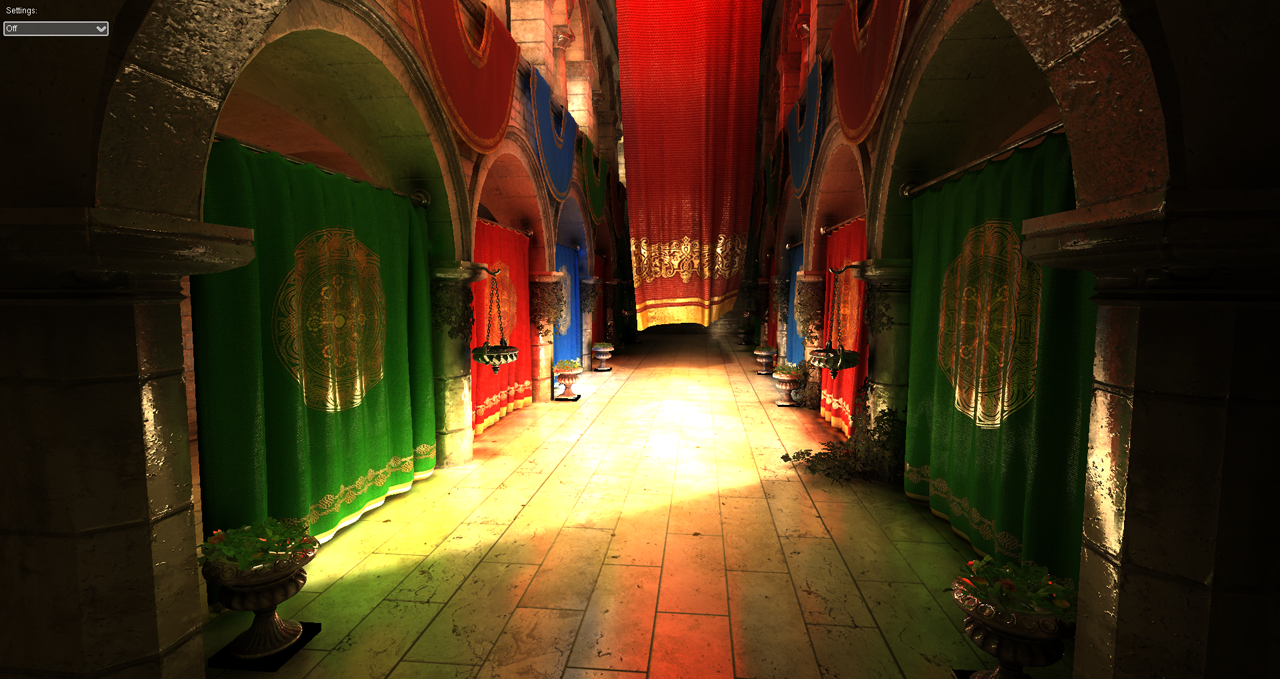
\includegraphics[width=0.9\linewidth]{media/givoxels_sponzanew1.png}
	\caption{Escena \emph{Sponza} renderizada utilizando trazado de conos con vóxeles para la iluminación indirecta \cite{CNSGE11b}.}
	\label{fig:givoxels_sponzanew1}
\end{figure}

El algoritmo comprende varios pasos: primero la información de la luz y escena son almacenados en las hojas de la estructura de árbol, este es el nivel más fino de la jerarquía. Luego estos valores son filtrados dentro del árbol disperso hacia todos los niveles de la jerarquía hasta llegar a la raíz. En un último paso para el cálculo de iluminación indirecta por cada fragmento, los valores dentro de esta jerarquía son recolectados sobre una semiesfera utilizando trazado de conos. En algoritmos como \emph{ray tracing} esta recolección de valores es lenta y es realizada por muchos rayos. Es de notar que todos estos rayos trazados sobre la semiesfera son direccional y espacialmente coherentes. \Ac{VCT} hace uso de este concepto para discretizar muchos rayos en simples conos.

\subsubsection{Construcción del Octree de Vóxeles}
\label{subsub:octree_building}
El algoritmo está pensando para funcionar con escenas dinámicas. Sin embargo las escenas son divididas entre partes dinámicas y estáticas para acelerar el proceso de voxelización con objetos dinámicos.

Primero la escena es renderizada utilizando proyección ortogonal. Cada triángulo es proyectado sobre uno de los ejes principales, este eje es seleccionado según la normal del triángulo, esto se hace para maximizar el área visible del triángulo con respecto al eje. Cada fragmento producto de esta proyección es almacenado en una lista de vóxeles-fragmentos junto a parámetros como posición en escena, normal y color. Para saber la cantidad de elementos que esta lista debe almacenar, primero se debe realizar una pasada contando el número de fragmentos con un contador atómico.

\begin{wrapfigure}{l}{0.4\linewidth}
	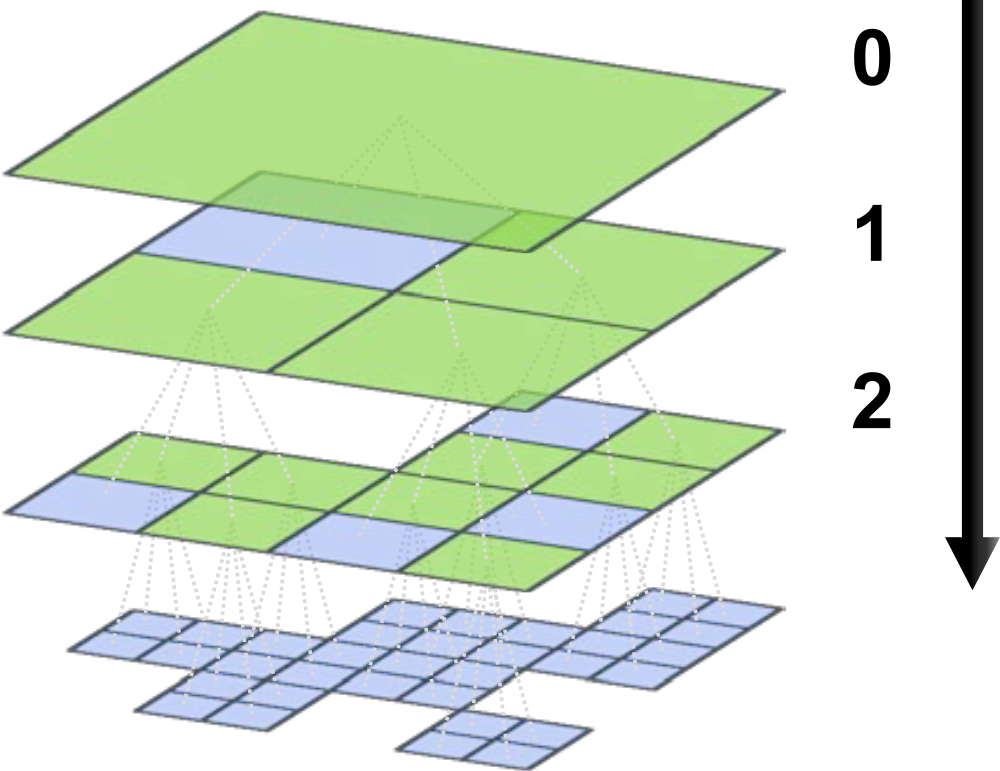
\includegraphics[width=0.95\linewidth]{media/miplevels.png}
	\caption{Descripción gráfica del proceso de subdivisión del octree.}
	\label{fig:miplevels}
\end{wrapfigure}
\noindent Una vez llena la lista de vóxeles-fragmentos, se genera un hilo de procesamiento por cada fragmento en la lista. Los fragmentos son introducidos en el árbol disperso que inicialmente solo tiene un nodo raíz (ver Figura \ref{fig:miplevels}). Cada vez que un nodo de este octree necesita ser dividido, un nuevo nodo es creado y se almacena sobre memoria ya reservada en la \ac{GPU}. La posición del nodo en memoria es determinada por un contador atómico, el cual se incrementa con cada nuevo nodo. Al inicio del proceso de subdivisión de los nodos se genera una gran cantidad de colisiones entre hilos, por esto cada nodo tiene asociado un símbolo mutex.

\subsubsection{Contenido de un Vóxel}
\label{subsub:voxelcontent_orig}

El algoritmo está diseñado para hacer uso de filtrado trilineal por hardware. Sin embargo dos vóxeles vecinos no necesariamente están posicionados de forma subsecuente en memoria. Por esto cada nodo contiene un bloque o \emph{brick}. Este bloque representa el entramado $3^3$ de la celda, donde estas celdas se encuentran en las esquinas de los hijos del nodo (ver Figura \ref{fig:bricks_vct}).

Cada vóxel representa varios parámetros, entre ellos color, opacidad, normal, intensidad, etc.

\begin{figure}[H]
	\centering
	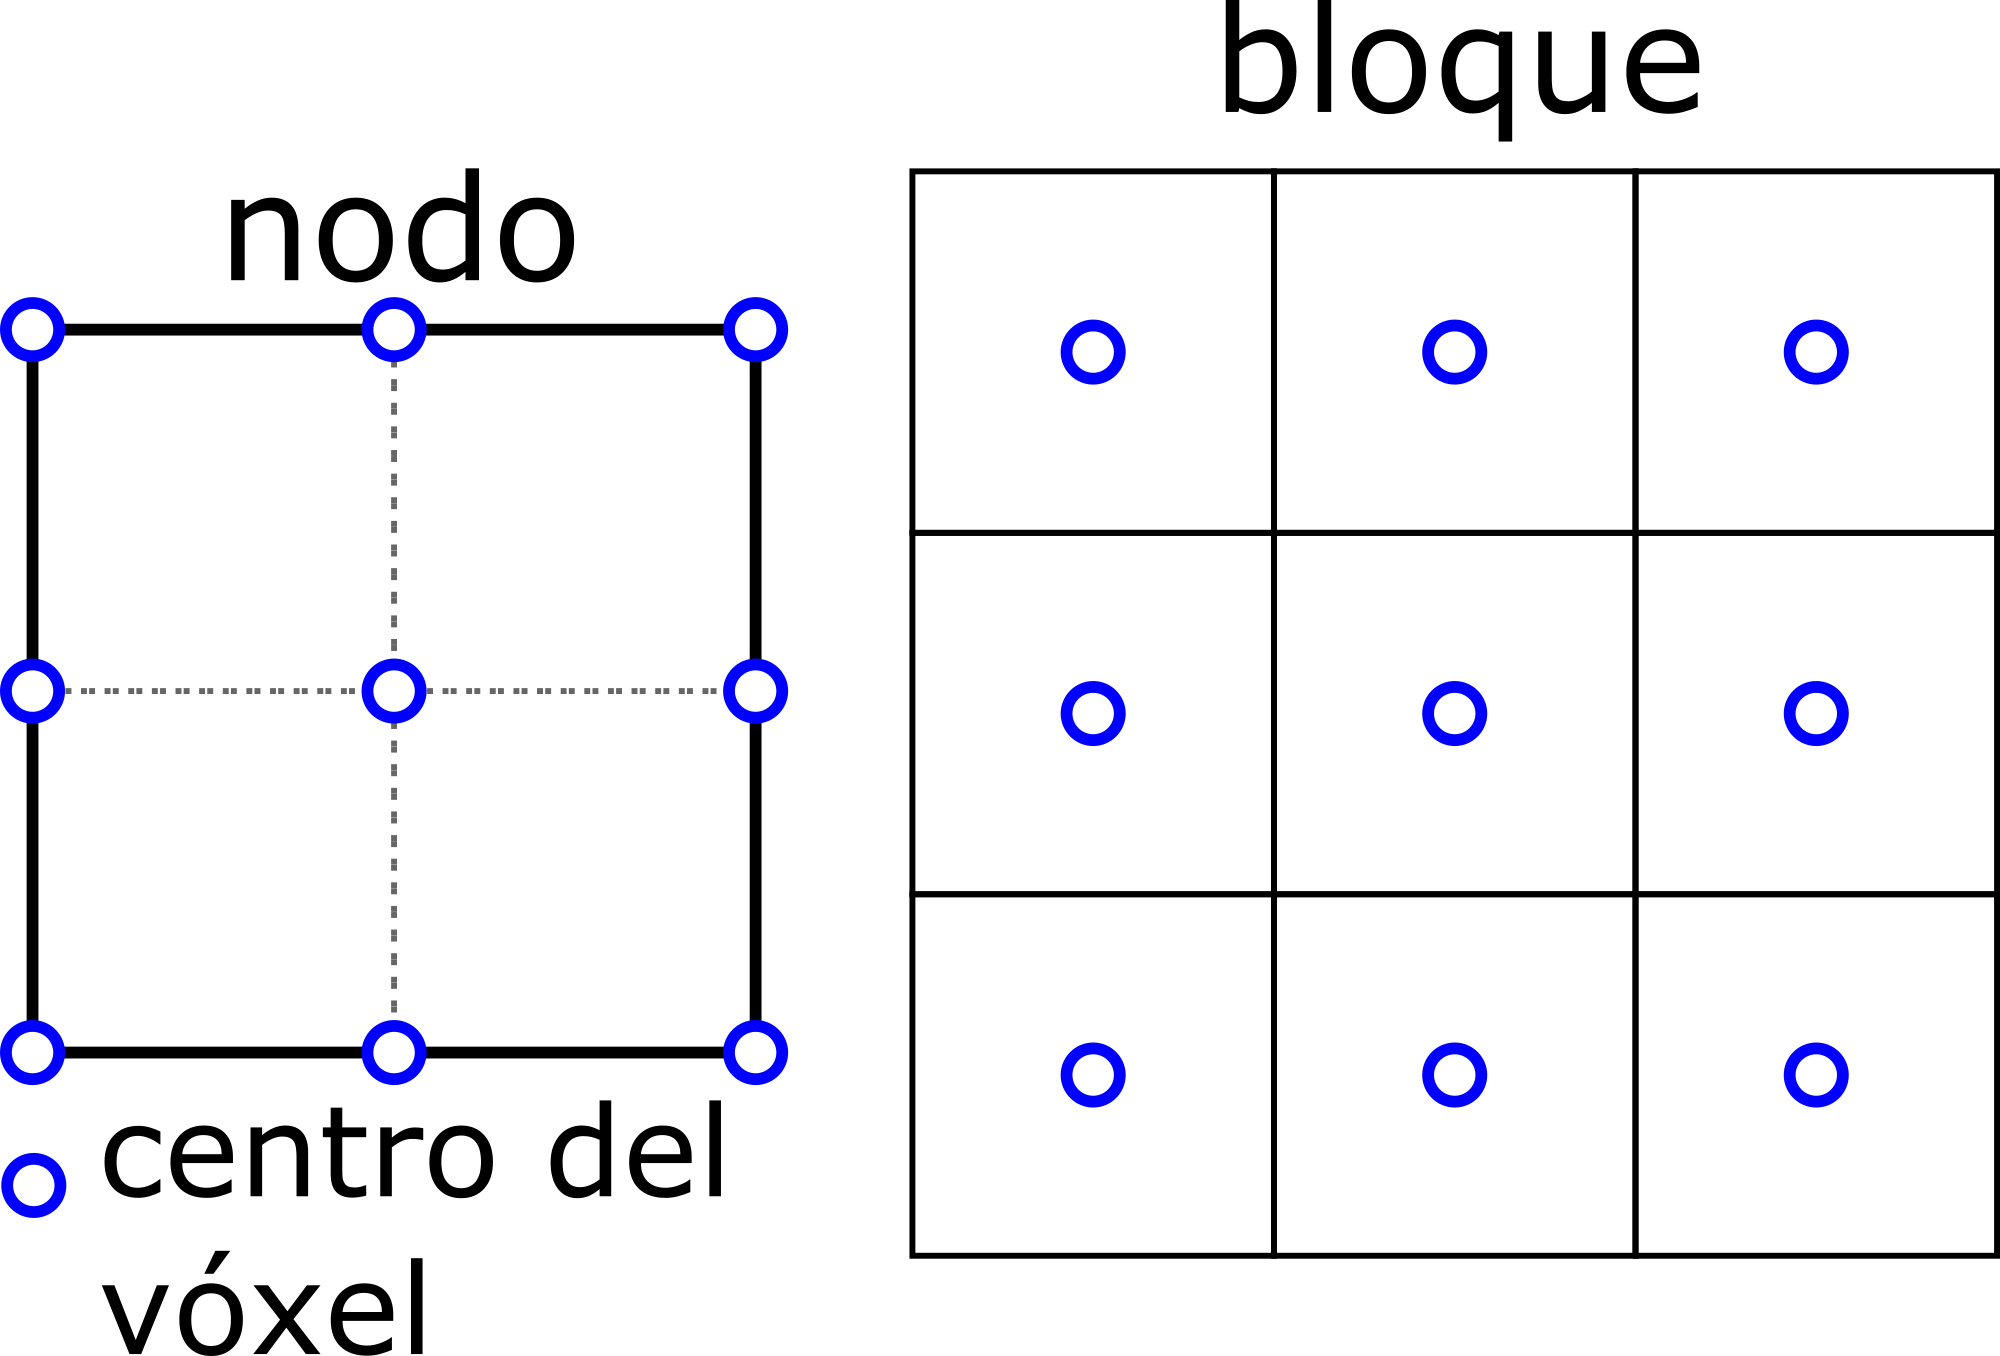
\includegraphics[width=0.3\linewidth]{media/bricks_vct.png}
	\caption{Bloques y nodos, los valores de los bloques se encuentran en las esquinas para rápido acceso y filtrado \cite{CNSGE11b}.}
	\label{fig:bricks_vct}
\end{figure}

\subsubsection{Filtrado en Niveles de Detalle}
\label{subsub:mipmaping_orig}
Inicialmente cada uno de estos parámetros es almacenado dentro de las hojas del árbol disperso. Luego de forma iterativa estos valores son filtrados desde los niveles más bajos a los niveles más altos de la jerarquía lo que resulta en distintos niveles de detalles para la escena voxelizada, este proceso es llamado \emph{mipmapping}. Cada nodo de un bloque es filtrado a partir de las $3^3$ celdas del nivel anterior en jerarquía. Para calcular el valor filtrado sobre el actual nodo el algoritmo promedia los valores de los nodos en el nivel anterior. Al calcular el valor filtrado cada vóxel debe ser pesado con la inversa de su multiplicidad, resultando en un kernel gaussiano de tamaño $3^3$. 

\subsubsection{Trazado de Conos y Vóxeles}
Una vez que el árbol disperso está filtrado y completo se utiliza para el cálculo de iluminación indirecta. Por cada fragmento un conjunto de conos es generado. La dirección y apertura de cada cono es determinada por la \ac{BRDF} del material en ese fragmento. Por ejemplo la \ac{BRDF} Blinn-Phong vista en la sección \ref{para:blinn_phong} puede ser descompuesta como un lóbulo ancho para la parte difusa y un lóbulo especular. Para el lóbulo difuso varios conos son generados orientados por la semiesfera sobre el punto con apertura y dirección maximizadas a tal manera que los conos cubran gran parte de la misma. Para el lóbulo especular se genera un solo cono con una apertura que varía según el término $n$ de la \ac{BRDF} Blinn-Phong. El cono especular tiene como dirección la dirección de la luz incidente reflectada $R$ (sección \ref{para:speculars}).

El algoritmo utiliza trazado de conos aproximado para acumular la intensidad de la luz incidente sobre el fragmento. Los valores son recolectados de varias muestras a través del recorrido del cono utilizando composición \emph{front-to-back}. Por cada muestra se examina el árbol disperso de vóxeles. El nivel del árbol a examinar es determinado por el diámetro del cono en esa posición.

%Por cada paso del trazado se obtiene un valor de oclusión $\alpha_{2}$ y valor de radiancia $c_2$. Para acumular los valores en muestreados a través del recorrido del cono se utiliza acumulación volumétrica \emph{front-to-back}. Para esto es necesario llevar pista de un valor oclusión $a$ y color $c$. La actualización de estos valores por cada paso se realiza de la siguiente manera: $c=c+(1-a)c_2$ y $a=a+(1-a)a_2$

\subsubsection{Filtrado Anisotrópico de Vóxeles.}
\label{subsub:aniso_voxels_orig}
A pesar de que el filtrado gaussiano es suficiente para proveer resultados visuales coherentes, algunos problemas de calidad visual pueden ocurrir bajo ciertas condiciones. El primer problema se conoce como el problema de la pared rojo-verde. Al promediar valores dentro del octree con dos vóxeles opacos con diferentes colores provenientes de por ejemplo, dos paredes planas, el color resultante del vóxel describe ambas paredes como si estas fueran transparentes. Otro problema resulta también de promediar opacidad entre vóxeles totalmente transparentes y vóxeles totalmente opacos, resultando un valor filtrado semitransparente. Esto puede resultar en fugas de luz a través de la geometría en la escena.

\begin{figure}[H]
	\centering
	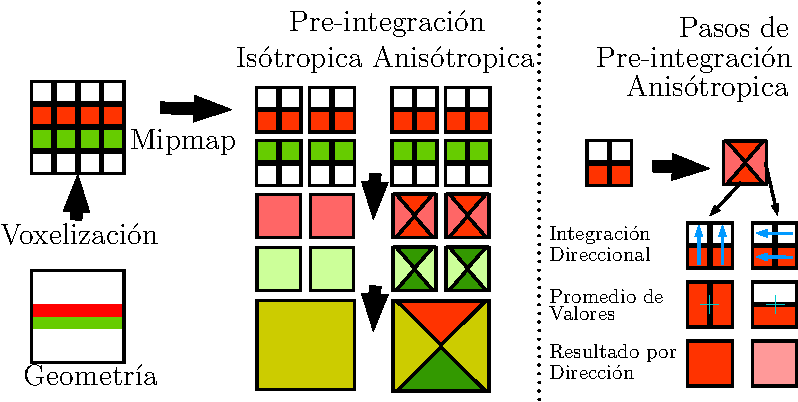
\includegraphics[width=0.90\linewidth]{media/isotropic_cropped.pdf}
	\caption{A la izquierda se describe el proceso de \emph{mipmapping} de vóxeles sin y con filtrado anisótropico. Los pasos para la integración direccional se observan a la derecha.}
	\label{fig:vct_anisofiltering}
\end{figure}

Para solventar este problema se realiza una representación anisotrópica de los vóxeles durante el proceso de \emph{mipmapping}. En vez de tener un solo canal de valores filtrados sin dirección, ahora los valores serán filtrados de forma direccional, almacenando seis canales por cada eje positivo y negativo. Un valor direccional es calculado realizando un paso de integración volumétrica en profundidad y promediando los cuatro valores direccionales para obtener el valor resultante según una dirección (ver Figura \ref{fig:vct_anisofiltering}).

\subsubsection{Captura de Iluminación Directa en Vóxeles}
\label{subsub:voxel_capture}
Para el cálculo de iluminación indirecta es necesario describir como la radiancia incidente es almacenada en los nodos del árbol. Este proceso está inspirado en \ac{RSM}, donde la escena es renderizada desde el punto de vista de la fuente de luz y se utiliza rasterización estándar para almacenar las posiciones de los fragmentos en una textura. Cada píxel en esta textura representa un fotón que rebota en escena. Esta textura se le llama mapa de luz-vista o \emph{light-view map}. Luego de generar este mapa es necesario almacenar los fotones en el árbol octree. Los fotones son almacenados como una distribución direccional y energía proporcional al casquete esférico del ángulo sólido del píxel visto desde la luz.

El procesamiento de la textura de fotones sobre el árbol se realiza en el procesador de fragmentos o \emph{fragment shader}. Como usualmente la dimensión del \emph{light-view map} es mayor a la resolución de la cuadrícula de vóxeles se puede asumir que los fotones serán almacenados directamente en las hojas del árbol octree. Además, los fotones siempre pueden ser almacenados en el nivel más fino de detalle en la representación con vóxeles porque estos describen información de la superficie geométrica. Es posible que muchos fotones terminen sobre un mismo vóxel, por esto es necesario utilizar adicción atómica para garantizar coherencia entre los hilos generados por cada fragmento.

  % propuesta de aplicacion
  \chapter{Solución Propuesta}
\label{chap:proposal}
  % implementacion de aplicacion
  \chapter{Implementación}
\label{chap:implementation}

\section{Herramientas}
Nuestra implementación para el cálculo de iluminación global en tiempo real está basada en la \ac{GPU}. Esta aplicación genera gráficos por computadora utilizando rasterización en tiempo real acelerado por hardware gráfico, para esto existen principalmente dos  API gráficas, OpenGL y Direct3D. Para acceder a distintas características del hardware gráfico, rasterización y pipeline de renderizado se utilizó OpenGL junto al lenguaje de sombreado GLSL para el desarrollo de shaders. 

La aplicación hace uso de características relativamente recientes en OpenGL como lectura y escritura arbitraria y operaciones atómicas sobre texturas utilizando la extensión ya mencionada en la sección \ref{sec:voxelizacion}. Esta extensión es parte del núcleo de OpenGL desde la versión 4.2. 

Otro aspecto importante de la aplicación es el uso de \ac{GPGPU} para distintos cálculos de iluminación, filtrado y sombreado sobre datos almacenados en volúmenes. El uso de \ac{GPGPU} nos permite realizar cálculo paralelo masivo utilizando núcleos dedicados en la \ac{GPU}. Para esto existen distintas alternativas como CUDA y OpenCL o recientemente \emph{compute shaders}. En nuestra aplicación se utilizaron \emph{compute shaders} los cuales provee OpenGL desde la versión 4.3. Estos shaders permiten cómputo general en la GPU con la sintaxis ya familiar de GLSL además de mayor compatibilidad en contraste con tecnologías como CUDA que solo están disponibles en tarjetas gráficas NVIDIA.

El lenguaje de desarrollo escogido fue C++ ya que este ofrece acceso directo al manejo de memoria similar al lenguaje C que está escrito OpenGL. Este acceso directo además ayuda a eliminar capas de abstracción sobre los datos que existen en otros lenguajes de más alto nivel. Esto puede ayudar a mejorar el rendimiento de la aplicación lo cual es importante para técnicas de renderizado en tiempo real. Otra razón importante por la que se escoge este lenguaje es que muchas herramientas utilizadas para facilitar el desarrollo de aplicaciones gráficas están escritas en este lenguaje. El entorno de desarrollo fue Visual Studio 2015 Community Edition en el sistema operativo Windows 10.

OpenGL necesita acceder al contexto o framebuffer de una ventana instanciada en algún sistema operativo para poder renderizar. Para la creación, manejo y acceso al contexto de ventanas se utilizó \emph{GLFW} versión 3.1.2. Para cargar las funciones de OpenGL, extensiones y enlazar el contexto se utilizó \emph{GLEW} en su versión 1.13.0. Para OpenGL en C++ a pesar de que se puede acceder directamente a sus funciones en crudo se utilizó un wrapper llamado \emph{OGLplus} en su versión 0.52.0. Este implementa una fachada orientada a objetos sobre OpenGL más acorde con el estilo de programación en C++. OGLplus provee administración automática de recursos y objetos de OpenGL, encapsulación y seguridad de tipos, manejo de errores e interoperabilidad con OpenGL en crudo. Para manejo de vectores y matrices además de otras funciones y operaciones matemáticas se utilizó la biblioteca GLM versión 0.9.7.

La aplicación hace uso de varios modelos, escenas tridimensionales y texturas, para estos recursos existen distintos formatos. Implementar soporte para una variedad de ellos es una tarea ardua por esto se utilizaron bibliotecas en C++ que ya proveen esta funcionalidad. Para la carga de mallas 3D e información de escena como cámaras, luces, materiales, jerarquía de objetos y texturas se utilizó la biblioteca \emph{Assimp} en su versión 3.2 por la variedad de formatos que soporta y las múltiples funciones que provee para pre-procesar los mallas e información de la escena. Para cargar datos en crudo de texturas se utilizó la biblioteca \emph{FreeImage}.

Para facilitar el uso de la aplicación esta provee una interfaz gráfica con acceso a distintas funciones relevantes a la manipulación de objetos en escena y parámetros del algoritmo de iluminación global. Para esto se utilizó la biblioteca \emph{dear imgui}, la cual provee distintas rutinas para la composición de interfaces de usuario, esta biblioteca utiliza el mismo pipeline de renderizado para dibujar la interfaz.

\section{Arquitectura de la Aplicación} % (fold)
\label{sec:arquitectura_de_la_aplicacion}
Detrás de la generación de frames se encuentra un sencillo motor gráfico compuesto por una multitud de clases extensibles. En esta sección se examina un poco la arquitectura de este. Sin embargo se hará énfasis detallado en las partes más relevantes al algoritmo de iluminación global.

Una escena en la aplicación está definida por cámaras, luces, materiales, texturas, mallados y un nodo raíz de jerarquía de escena.

\begin{figure}[H]
	\centering
	\captionsetup{justification=centering}
	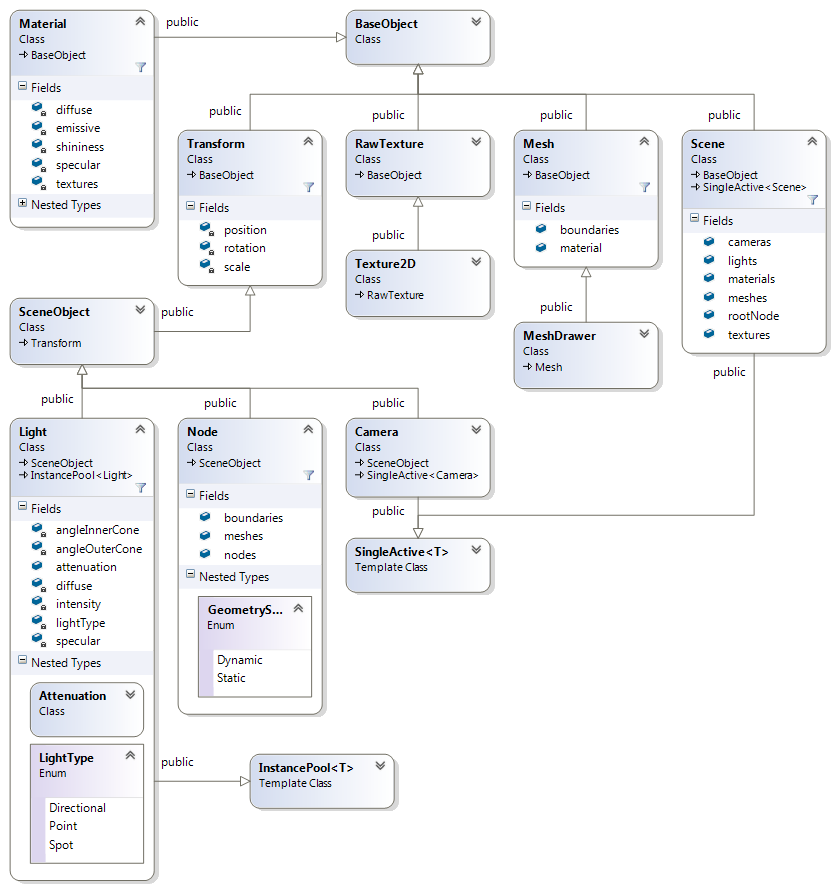
\includegraphics[width=\linewidth]{media/ClassDiagram1.png}
	\caption{Diagrama de clases relevantes para la definición de escenas en el motor gráfico para el renderizado de iluminación global.}
\end{figure}

Como se observa en el diagrama cada \emph{Node} o nodo tiene un grupo \emph{meshes} o mallados asociado. Cada una de estas \emph{Mesh} o mallas tiene un material (clase \emph{Material}) asignado, este material puede o no tener uso de texturas. Los nodos en la escena puede definirse como estáticos o dinámicos, esta propiedad es importante para diferenciar entre voxelización estática y dinámica.

Se puede observar también que tanto nodos como mallas tienen un miembro \emph{boundaries} o delimítate, este miembro define una \ac{AABB} utilizada para determinar si estos objetos se encuentra dentro del tronco cuadrado que define el volumen de proyección de la cámara. Esta técnica es llamada \emph{frustum culling}. 

Existen tres tipos de luces en nuestra implementación como ya fue mencionado anteriormente: luces direccionales, puntuales y focales. Una de las ventajas de realizar el sombreado a través de compute shaders es que podemos colocar muchas luces en escena sin necesidad de crear mapas luz-vista por cada uno de estos.

\begin{figure}[H]
	\centering
	\captionsetup{justification=centering}
	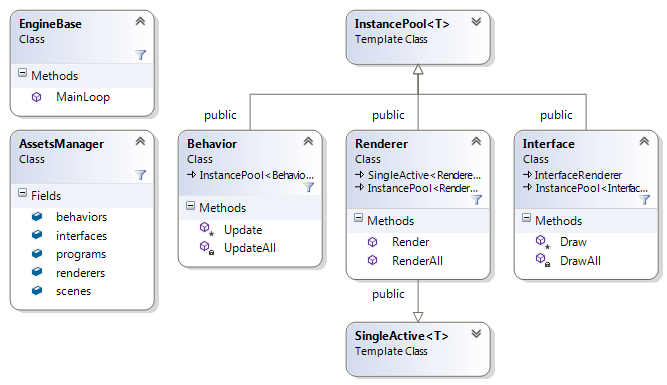
\includegraphics[width=\linewidth]{media/ClassDiagram.png}
	\caption{Diagrama de principales clases con métodos abstractos relacionados con la actualización de cada frame.}
\end{figure}

La aplicación utiliza abstracción en el \emph{loop} o ciclo de renderizado. Existen tres clases bases las cuales proveen un método abstracto a implementar por los hijos de estas. Las clases que implementan estos métodos son instanciadas en la clase \emph{AssetsManager}. Por cada instancia de estas clases cada uno de estos métodos es llamado con cada iteración del ciclo de renderizado. Este ciclo incluye la actualización de interfaces, actualización de lógica y actualización de renderizado.

En el diagrama observamos la clase base \emph{Renderer}. En nuestra implementación la voxelización, actualización del mapa de sombras y el cálculo de iluminación global son implementados en clases que heredan de Renderer. La clase \emph{Interface} es la base de todas las interfaces en la aplicación. Mientras que la clase \emph{Behavior} solo es utilizada para lógica de cámara libre flotante en escena.

\begin{figure}[H]
	\centering
	\captionsetup{justification=centering}
	\includegraphics[width=\linewidth]{media/mainloopflow.pdf}
	\caption{Descripción del flujo de ejecución del método \emph{MainLoop} en donde reside el ciclo de renderizado.}
\end{figure}

Los métodos \emph{Render}, \emph{Draw} y \emph{Update} son abstractos. Mientras que los métodos \emph{RenderAll}, \emph{UpdateAll} y \emph{DrawAll} son métodos estáticos públicos accesibles por la clase \emph{EngineBase}. Estos métodos estáticos invocan a todos las implementaciones de los métodos abstractos por cada clase que hereda de Renderer, Interface o Behavior respectivamente. El método MainLoop en EngineBase por tanto se abstrae de la implementación de estos métodos y simplemente invoca todas las implementaciones por cada nuevo frame.
% section arquitectura_de_la_aplicacion (end)

\section{Pipeline de Voxelización} % (fold)
\label{sec:pipeline_de_voxelizacion}
El algoritmo de voxelización de escenas es implementado en una clase que hereda de la clase Renderer. En el método Render, residen la lógica por el lado de la CPU de voxelización, sombreado de vóxeles, mipmapping para vóxeles anisótropos e iluminación global de vóxeles. En esta sección se describe en detalle solo el proceso de voxelización y su arquitectura.
\subsection{Arquitectura}

La arquitectura de nuestro proceso de voxelización describe un pipeline, donde la entrada es geometría, materiales, texturas y matrices de proyección y la salida es una serie de volúmenes de vóxeles los cuales describen una discretización de esta geometría.

El algoritmo de voxelización se ejecuta entre el geometry shader y el fragment shader. En el geometry shader se proyecta y traslada los vértices de cada triángulo para generar un triángulo expandido. La rasterización conservativa de cada triángulo es tarea de ambos shaders. El fragment shader primeramente descarta fragmentos excedentes de la expansión del triángulo en el geometry shader para formar un polígono delimitante. La voxelización de geometría estática y dinámica se realiza sobre este mismo pipeline, el fragment shader debe garantizar que los vóxeles estáticos no sean sobrescritos, finalmente se realiza una operación de promedio sobre todos los atributos de cada fragmento que forma parte del espacio que envuelve un vóxel, este valor es almacenado luego en cada vóxel por atributo. En la Figura \ref{fig:voxel_pipeline_impl} se ilustra esta arquitectura.
\begin{figure}[H]
    \centering
    \includegraphics[width=\linewidth]{media/voxel_pipeline_cropped.pdf}
    \caption{Descripción gráfica del pipeline de voxelización.}
    \label{fig:voxel_pipeline_impl}
\end{figure}

\subsection{Voxelización Conservativa} % (fold)
\label{sub:voxelization_impl}
Nuestra implementación utiliza una representación simplificada de la escena en vóxeles, esta representación es generada de forma conservativa por tanto si existe algún triángulo dentro del espacio de un vóxel se generara un vóxel por más pequeño que sea este triángulo.
 
\subsubsection{Matrices de Proyección por Eje}

Como se explicó en la sección \ref{sub:voxelizacion_conservativa} cada triángulo debe ser proyectado sobre un eje direccional. El primer paso a realizar es definir estas matrices de proyección. Estas están definidas por una \ac{AABB} uniforme. En nuestra implementación se toma la \ac{AABB} que envuelve toda la escena por simplicidad. En el código \ref{UpdateProjectionMatrices} se encuentra el algoritmo de la función que realiza esto. Este método se invoca cada vez que se carga una escena o cuando se cambia la resolución de la representación en vóxeles.

La \ac{AABB} puede estar definida de dos formas: por un punto que indica el centro de la caja y un vector extensión que indica la longitud media de la caja en cada eje a partir del centro o por un punto mínimo y un punto máximo. 
\\
\begin{lstlisting}[caption={Creación de matrices de proyección ortogonal por cada eje direccional}, label=UpdateProjectionMatrices]
void VoxelizerRenderer::UpdateProjectionMatrices(const BoundingBox &sceneBox)
{
    // longitud del aabb en cada eje
    auto axisSize = sceneBox.Extent() * 2.0f;
    // centro del aabb
    auto &center = sceneBox.Center();
    // tamaño de la cuadrícula de vóxeles
    volumeGridSize = glm::max(axisSize.x, glm::max(axisSize.y, axisSize.z));
    // tamaño de un vóxel en la cuadrícula
    voxelSize = volumeGridSize / volumeDimension;
    auto halfSize = volumeGridSize / 2.0f;
    // proyección ortogonal
    auto projection = glm::ortho(-halfSize, halfSize, -halfSize, halfSize, 0.0f, volumeGridSize);
    // matrices de vista por cada eje
    viewProjectionMatrix[0] = lookAt(center + glm::vec3(halfSize, 0.0f, 0.0f), center, glm::vec3(0.0f, 1.0f, 0.0f));
    viewProjectionMatrix[1] = lookAt(center + glm::vec3(0.0f, halfSize, 0.0f), center, glm::vec3(0.0f, 0.0f, -1.0f));
    viewProjectionMatrix[2] = lookAt(center + glm::vec3(0.0f, 0.0f, halfSize), center, glm::vec3(0.0f, 1.0f, 0.0f));
    // multiplicación de ambas matrices para obtener la matriz de proyección para los triángulos
    for (auto &matrix : viewProjectionMatrix) { matrix = projection * matrix; }
}
\end{lstlisting}

En el Código \ref{UpdateProjectionMatrices} se observa que primero se obtiene la longitud total en cada eje que define la \ac{AABB} que envuelve la escena. Luego en la misma función se actualizan dos variables: \emph{volumeGridSize} que indica el tamaño de la cuadrícula tridimensional de vóxeles en espacio de mundo y \emph{voxelSize} que indica el tamaño de cada vóxel dentro de esta cuadrícula. 

El tronco de proyección es un cubo uniforme por tanto se utiliza la mayor longitud según cada eje. Esto asegura que desde cualquier eje direccional la proyección abarca toda la escena. De esta longitud se extrae la matriz de proyección ortogonal. Luego se configura cada matriz de vista por cada eje direccional. Finalmente se almacena la multiplicación de ambas matrices.

Una vez obtenidas las matrices de proyección el algoritmo procede a voxelizar la escena. El proceso de voxelización estática y dinámica utilizan el mismo programa de sombreado o \emph{shader}, la diferencia reside sobre cual geometría es enviada al pipeline de rasterización y durante el fragment shader si se lee o se escribe sobre una textura que indica las posiciones de vóxeles estáticos.

\subsubsection{Selección del Eje Dominante}
Para maximizar el área de voxelización y generar la mayor cantidad de fragmentos posibles cada triángulo es proyectado sobre uno de los ejes direccionales. Este eje se escoge según la normal definida por el plano formado por los tres vértices del triángulo. Este proceso se realiza en el geometry shader. En el geometry shader se puede realizar operaciones sobre los vértices generados por el procesador de vértices o \emph{vertex shader}. Esto es de particular interés para el proceso de voxelización conservativa ya que como fue explicado anteriormente cada vértice de cada triángulo necesita ser expandido.
\\
\begin{lstlisting}[caption={Selección del eje dominante para la proyección ortogonal.}, label=CalculateAxis]
int CalculateAxis()
{
    // normal del plano formado por vertices del triangulo
    vec3 p1 = gl_in[1].gl_Position.xyz - gl_in[0].gl_Position.xyz;
    vec3 p2 = gl_in[2].gl_Position.xyz - gl_in[0].gl_Position.xyz;
    vec3 faceNormal = cross(p1, p2);

    // valor por eje direccional
    float nDX = abs(faceNormal.x);
    float nDY = abs(faceNormal.y);
    float nDZ = abs(faceNormal.z);

    // índice para la matriz de proyección
    if( nDX > nDY && nDX > nDZ )
    {
        return 0;
    }
    else if( nDY > nDX && nDY > nDZ  )
    {
        return 1;
    }
    else
    {
        return 2;
    }
}
\end{lstlisting}

En el Código \ref{CalculateAxis} primero se obtiene la normal del triángulo. El arreglo \emph{gl\_in} contiene información de todos los vértices generados por el vertex shader. Para la aplicación esto es forzado a solo triángulos, por tanto la longitud de gl\_in siempre es tres. Luego según el peso en cada eje del vector normal del plano formado por el triángulo se escoge un eje direccional. Esto se retorna como un número entero. Este número indica cuál de las matrices de proyección generadas en la sección anterior va ser utilizada para proyectar cada vértice del triángulo. En la Figura \ref{fig:axis_selection} se ilustra este proceso.

\begin{figure}[H]
	\centering
	\begin{subfigure}[t]{.49\linewidth}
		\centering
		\captionsetup{justification=centering}
		\includegraphics[width=\linewidth]{media/Voxelization_blog_fig_5.png}
		\caption*{Tres direcciones potenciales de proyección.}
	\end{subfigure}%
	\hspace{0.01\textwidth}
	\begin{subfigure}[t]{.49\linewidth}
		\centering
		\captionsetup{justification=centering}
		\includegraphics[width=\linewidth]{media/Voxelization_blog_fig_6.png}
		\caption*{Según la normal, proyección al eje Y es lo indicado.}
	\end{subfigure}%
	\caption{Descripción gráfica del proceso de selección del eje de proyección \cite{gpuvoxelization}.}
	\label{fig:axis_selection}
\end{figure}

\subsubsection{Extensión del Triángulo y Polígono Delimitante}
Una vez proyectados todos los vértices del triángulo según el eje direccional escogido (esto es multiplicar cada vértice por la matriz escogida) entonces se procede a expandir los vértices de este triángulo. Antes de esto primero es importante definir una \ac{AABB} para el triángulo. Esta area delimitante es utilizada en el fragment shader para descartar fragmentos excedentes del triángulo expandido. El punto mínimo y máximo se expanden según la longitud diagonal de un pixel, en nuestra implementación este valor es $\frac{1}{V_{res}}$ donde $V_{res}$ representa la resolución del volumen. El Código \ref{AxisAlignedBoundingBox} expone como se genera este \ac{AABB}.  El arreglo \emph{pos} contiene los vértices del triángulo proyectado
\\
\begin{lstlisting}[caption={Creación de un \ac{AABB} para el triángulo proyectado.}, label=AxisAlignedBoundingBox]
vec4 AxisAlignedBoundingBox(vec4 pos[3], vec2 pixelDiagonal)
{
    vec4 aabb;
    // punto mínimo y máximo para definir el aabb
    aabb.xy = min(pos[2].xy, min(pos[1].xy, pos[0].xy));
    aabb.zw = max(pos[2].xy, max(pos[1].xy, pos[0].xy));
    // se extiende el aabb por la longitud diagonal de un píxel
    aabb.xy -= pixelDiagonal;
    aabb.zw += pixelDiagonal;
    return aabb;
}
\end{lstlisting}

Primero se calculan los planos perpendiculares al triángulo formados por cada par de vértices del triángulo. Estos planos son trasladados medio pixel hacia afuera con respecto al triángulo proyectado. El Código \ref{TPlanes} muestra cómo se calculan estos planos.
\\
\begin{lstlisting}[caption={Planos por cada par de vértices del triángulo proyectado.}, label=TPlanes]
vec2 halfPixel = vec2(1.0f / volumeDimension);
// cálculo de planos perpendiculas al triangulo
// segun los vertices en formato normal-distancia
vec3 planes[3];
planes[0] = cross(pos[0].xyw - pos[2].xyw, pos[2].xyw);
planes[1] = cross(pos[1].xyw - pos[0].xyw, pos[0].xyw);
planes[2] = cross(pos[2].xyw - pos[1].xyw, pos[1].xyw);
planes[0].z -= dot(halfPixel, abs(planes[0].xy));
planes[1].z -= dot(halfPixel, abs(planes[1].xy));
planes[2].z -= dot(halfPixel, abs(planes[2].xy));
\end{lstlisting}

Luego se calcula la intersección entre los planos perpendiculares al triángulo. El Código \ref{TPlanes2} muestra el cálculo de estas intersecciones.
\\
\begin{lstlisting}[caption={Intersección entre planos perpendiculares al triángulo proyectado.}, label=TPlanes2]
// puntos de intersección entre los planos perpendiculares
vec3 intersection[3];
intersection[0] = cross(planes[0], planes[1]);
intersection[1] = cross(planes[1], planes[2]);
intersection[2] = cross(planes[2], planes[0]);
intersection[0] /= intersection[0].z;
intersection[1] /= intersection[1].z;
intersection[2] /= intersection[2].z;
\end{lstlisting}

Finalmente se obtienen los vértices del triángulo expandido. El Código \ref{TPlanes3} la composición final de cada vértice el triángulo.
\\
\begin{lstlisting}[caption={Vértices del triángulo expandido.}, label=TPlanes3]
vec4 trianglePlane;
// plano del triángulo proyectado
trianglePlane.xyz = cross(pos[1].xyz - pos[0].xyz, pos[2].xyz - pos[0].xyz);
trianglePlane.xyz = normalize(trianglePlane.xyz);
trianglePlane.w = -dot(pos[0].xyz, trianglePlane.xyz);
// dilatación de los vértices del triangulo
float z[3];
z[0] = (-intersection[0].x * trianglePlane.x - intersection[0].y * trianglePlane.y - trianglePlane.w) / trianglePlane.z;
z[1] = (-intersection[1].x * trianglePlane.x - intersection[1].y * trianglePlane.y - trianglePlane.w) / trianglePlane.z;
z[2] = (-intersection[2].x * trianglePlane.x - intersection[2].y * trianglePlane.y - trianglePlane.w) / trianglePlane.z;
// posición final de los tres vértices del triángulo expandido
pos[0].xyz = vec3(intersection[0].xy, z[0]);
pos[1].xyz = vec3(intersection[1].xy, z[1]);
pos[2].xyz = vec3(intersection[2].xy, z[2]);
\end{lstlisting}

Este nuevo triángulo expandido es enviado al pipeline de rasterización donde cada fragmento generado será procesado por el fragment shader. En el fragment shader se almacenara los datos de la escena sobre cada volumen de vóxeles.

\subsubsection{Composición de Fragmentos y Vóxeles}

Este proceso se realiza en el fragment shader. En la sección anterior se mencionó la creación de una \ac{AABB} para el triángulo expandido. Lo primero a realizar durante la composición de fragmentos es descartar los fragmentos excedentes del triángulo. El Código \ref{TPlanes4} expone este proceso.
\\
\begin{lstlisting}[caption={Descarte de fragmentos excedentes en el fragment shader.}, label=TPlanes4]
// posición del fragmento debe encontrarse dentro del aabb
if( In.position.x < In.triangleAABB.x || In.position.y < In.triangleAABB.y || 
	In.position.x > In.triangleAABB.z || In.position.y > In.triangleAABB.w )
{
	discard;
}
\end{lstlisting}

Si la posición del fragmento esta fuera de la \ac{AABB} del triángulo este fragmento no es procesado. Esto resulta finalmente en un polígono delimitante ya descrito en la Figura \ref{fig:expanded_bbpolygon}.

Una vez ya finalizada la rasterización conservativa de cada triángulo, ahora se procede a almacenar información de la escena en texturas tridimensionales. En nuestra aplicación se almacena en vóxeles el albedo, normal, y emisión de la geometría en escena. Un vóxel puede envolver a varios fragmentos y cada uno de estos fragmentos puede tener distintos valores para los atributos mencionados. Una forma simple de almacenar todos estos valores es utilizando un promedio de todos los valores por fragmento que envuelve el vóxel. 

Como se mencionó en la seccion \ref{sub:frag_voxels}: cada fragmento es tratado como un hilo individual por tanto no hay forma de saber el orden en el que se envían fragmentos a la posición de un vóxel. La extensión \emph{GL\_ARB\_shader\_image\_load\_store} provee instrucciones atómicas para solventar esto. La forma más simple de obtener un promedio consistiria en utilizar la función \emph{imageAtomicAdd} y luego dividir por la cantidad de fragmentos. Para mantener un conteo de estos fragmentos se necesita un contador por cada vóxel. La idea es utilizar el canal alfa en un formato RGBA como contador. 

Sin embargo todas las funciones atómicas en esta extensión solo están reservadas para imágenes con formato entero de 32 bits. Generalmente el formato apropiado para estos valores seria RGBA8 o RGBA16F. Por tanto la función \emph{imageAdd} no puede ser utilizada para este propósito.

Se utiliza entonces la función \emph{atomicCompSwap} para emular la adición atómica. La idea es iterar por cada escritura sobre el volumen hasta que ya no haya más conflictos entre fragmentos y el valor actual del vóxel no ha sido cambiado por otro hilo de algún fragmento.

El promedio en cada vóxel debe ser calculado de forma incremental. Con el formato RGBA8 solo 8 bits están disponibles por canal. Por tanto es sencillo sobrepasar el valor límite de este formato mientras se suman valores. Para hacer esto se utiliza la siguiente formula:

\begin{equation}
	C_{i+1} = \frac{iC_{i}+x_i+1}{i+1}
\end{equation}

El Código \ref{imageAtomicRGBA8Avg} expone este procedimiento y la conversión entre formato RGBA8 y R32UI, sobre este último formato es posible realizar operaciones atómicas.
\\
\begin{lstlisting}[caption={Conversion entre RGBA8 y R32UI y promedio incremental.}, label=imageAtomicRGBA8Avg]
// conversion de formato de entero en r32ui a vec4
vec4 convRGBA8ToVec4(uint val)]
{
    return vec4(float((val & 0x000000FF)), 
    float((val & 0x0000FF00) >> 8U), 
    float((val & 0x00FF0000) >> 16U), 
    float((val & 0xFF000000) >> 24U));
}
// conversion de formato vec4 a entero r32ui
uint convVec4ToRGBA8(vec4 val)
{
    return (uint(val.w) & 0x000000FF) << 24U | 
    (uint(val.z) & 0x000000FF) << 16U | 
    (uint(val.y) & 0x000000FF) << 8U | 
    (uint(val.x) & 0x000000FF);
}
// promedio con atomicidad
void imageAtomicRGBA8Avg(layout(r32ui) volatile coherent uimage3D grid, ivec3 coords, vec4 value)
{
    // conversión de 0->1 de 0->255
    value.rgb *= 255.0;
    // valor equivalente en entero sin signo
    uint newVal = convVec4ToRGBA8(value);
    uint prevStoredVal = 0;
    uint curStoredVal;
    uint numIterations = 0;

    // mientras el valor almacenado sea diferente al actual y 
    // no se sobrepase el numero máximo de iteraciones
    while((curStoredVal = imageAtomicCompSwap(grid, coords, prevStoredVal, newVal)) 
            != prevStoredVal
            && numIterations < 255)
    {
        prevStoredVal = curStoredVal;
        vec4 rval = convRGBA8ToVec4(curStoredVal);
        rval.rgb = (rval.rgb * rval.a); // De-normalizar
        vec4 curValF = rval + value;    // Agregar nuevo valor
        curValF.rgb /= curValF.a;       // Re-normalizar
        newVal = convVec4ToRGBA8(curValF);
        ++numIterations;
    }
}
\end{lstlisting}

Esta función es llamada por cada fragmento para almacenar la normal, el albedo y la emisión del promedio de todos los fragmentos sobre el espacio que envuelve un vóxel, estos vóxeles se almacenan en texturas tridimensionales. El Código \ref{Voxelization2} ilustra el uso de la funcion \emph{imageAtomicRGBA8Avg} para almacenar cada atributo en volúmenes.
\\
\begin{lstlisting}[caption={Composición de fragmentos y vóxeles}, label=Voxelization2]
// volúmenes utilizados para almacenar información de escena en vóxeles
layout(binding = 0, r32ui) uniform volatile coherent uimage3D voxelAlbedo;
layout(binding = 1, r32ui) uniform volatile coherent uimage3D voxelNormal;
layout(binding = 2, r32ui) uniform volatile coherent uimage3D voxelEmission;

void main()
{
(*@\centerline{\raisebox{-1pt}[0pt][0pt]{$\vdots$}}@*)
    // llamadas al promedio atómico por fragmento
    imageAtomicRGBA8Avg(voxelNormal, position, normal);
    imageAtomicRGBA8Avg(voxelAlbedo, position, albedo);
    imageAtomicRGBA8Avg(voxelEmission, position, emissive);
(*@\centerline{\raisebox{-1pt}[0pt][0pt]{$\vdots$}}@*)
}
\end{lstlisting}

\subsubsection{Bandera Estática}
El proceso de voxelización para geometría estática y dinámica es el mismo. Como se explicó en la sección \ref{sub:voxelizacion_dinamica} en nuestra implementación se evitó la creación de nuevos volúmenes para vóxeles estáticos y dinámicos. Para garantizar esto se utiliza un volumen con un solo componente entero, formato R8.

Durante la voxelización estática se almacena en este volumen un valor para marcar esta posición como estática (en este caso valor 1). El Código \ref{Voxelization3} expone esta escritura. 
\\
\begin{lstlisting}[caption={Escritura de la bandera estática durante voxelización de geometría estática}, label=Voxelization3]
layout(binding = 3, r8) uniform image3D staticVoxelFlag;

void main()
{
(*@\centerline{\raisebox{-1pt}[0pt][0pt]{$\vdots$}}@*)
    // durante voxelización estática se escribe la bandera sobre el volumen
    if(flagStaticVoxels)
    {
        imageStore(staticVoxelFlag, position, vec4(1.0));
    }
(*@\centerline{\raisebox{-1pt}[0pt][0pt]{$\vdots$}}@*)
}
\end{lstlisting}

En contraste durante la voxelización dinámica se lee este volumen para descartar la escritura sobre vóxeles estáticos. El Código \ref{Voxelization4} expone esta lectura y descarte del fragmento.
\\
\begin{lstlisting}[caption={Lectura de la bandera estática durante voxelización de geometría dinámica.}, label=Voxelization4]
(*@\centerline{\raisebox{-1pt}[0pt][0pt]{$\vdots$}}@*)
    // durante voxelización dinámica se lee la bandera sobre el volumen
    if(!flagStaticVoxels)
    {
        bool isStatic = imageLoad(staticVoxelFlag, position).r > 0.0f;
        // si la posición del vóxel es estática se descarta el fragmento cancelando la escritura
        if(isStatic) { discard; }
    }
(*@\centerline{\raisebox{-1pt}[0pt][0pt]{$\vdots$}}@*)
\end{lstlisting}

\subsection{Revoxelización y Limpieza de Volúmenes}
Cada vez que se revoxeliza la escena los volúmenes utilizados durante el proceso de voxelización deben ser limpiados antes de usarse. Para la voxelización estática esto es sencillo, OpenGL provee una función llamada \emph{glClearImage} desde la versión 4.4 la cual permite llenar una textura con un valor indicado. Debido a que utilizamos el mismo volumen para la voxelización dinámica no podemos utilizar esta función durante la voxelización dinámica ya que se eliminarían todos los vóxeles estáticos.

Para solventar esto antes de llamar al proceso de voxelización con la geometría dinámica se limpian del volumen todos los vóxeles que no son estáticos utilizando un compute shader. El Código \ref{ClearVoxels} describe este proceso.
\\
\begin{lstlisting}[caption={Limpieza de vóxeles no estáticos.}, label=ClearVoxels]
void main()
{
    int volumeDimension = imageSize(voxelAlbedo).x;

    if(gl_GlobalInvocationID.x >= volumeDimension ||
        gl_GlobalInvocationID.y >= volumeDimension ||
        gl_GlobalInvocationID.z >= volumeDimension) return;

    ivec3 writePos = ivec3(gl_GlobalInvocationID);
    // vóxel vacío
    if(imageLoad(voxelAlbedo, writePos).a < EPSILON) { return; }
    // vóxel es estático
    if(texelFetch(staticVoxelFlag, writePos, 0).r > EPSILON) { return; }
    // vóxel no es estático entonces se procede a limpiar el volumen con ceros
    imageStore(voxelAlbedo, writePos, vec4(0.0));
    imageStore(voxelNormal, writePos, vec4(0.0));
    imageStore(voxelEmissive, writePos, vec4(0.0));
}
\end{lstlisting}

Primero se verifica si ya el vóxel está vacío, luego si este es estático y finalmente si este no lo es se le coloca el valor cero en todos los canales de color y el alfa, esto indica que allí no hay un vóxel.
% section pipeline_de_voxelizacion (end)

\section{Sombreado de Vóxeles} % (fold)
\label{sec:sombreado_de_voxeles_impl}
Para calcular la iluminación indirecta es necesario sombrear los vóxeles. Cada vóxel representa una simplificación de la radiancia saliente sobre un espacio en la escena. Llamaremos a la textura tridimensional resultante del sombreado de voxeles, \emph{textura base}. Esta información es utilizada por el algoritmo de trazado de conos para calcular la radiancia incidente sobre un fragmento.

En nuestra implementación la iluminación de los vóxeles comprende solo el componente difuso. En el proceso de voxelización se puede observar que ningún volumen está relacionado al componente especular de un material. Esto debido a dos razones: primero memoria ya que para incluir la especular durante el sombreado de vóxeles tendría que crearse otro volumen y segundo que usualmente el componente especular es un detalle fino de alta frecuencia, la voxelización siendo una simplificación de la escena podría perder detalle en especulares con lóbulos finos e incluso ocasionar errores de sombreado.

Para la iluminación de los vóxeles se utilizan técnicas de iluminación estándar en computación gráfica. La \ac{BRDF} de Lambert ya se encuentra almacenada en nuestro volumen albedo. Es necesario entonces multiplicar este valor por la atenuación normal, ignorando la emitancia:

\begin{equation}
	\begin{split}
		L(x\to\Theta) &= \int_{\Omega_{x}}{f_{r}(x, \Psi\to\Theta)L(x\gets\Psi)\cos(N_{x}, \Psi)dw_{\Psi}}\\
		&= \int_{\Omega_{x}}{\frac{\rho}{\pi}L(x\gets\Psi)\cos(N_{x}, \Psi)dw_{\Psi}}
	\end{split}
	\label{eq:shading_voxels}
\end{equation}

En nuestra implementación con solo iluminación directa esto equivale al siguiente código:
\\
\begin{lstlisting}[caption={Sombreado estándar para un vóxel}, label=Shading]
vec3 BRDF(Light light, vec3 normal, vec3 albedo)
{
	float nDotL = max(dot(normal, light.direction), 0.0f);
	return light.diffuse * albedo * nDotL;
}
\end{lstlisting}

\begin{wrapfigure}{l}{0.3\linewidth}
	\centering
	\captionsetup{justification=centering}
	\includegraphics[width=\linewidth]{media/gimped_normals.pdf}
	\caption{Normales disparejas en un vóxel.}
	\label{fig:error_normals}
\end{wrapfigure}
Calcular el sombreado de vóxeles de esta forma es suficiente para generar resultados de buena calidad sobre el trazado de conos. Sin embargo uno de los problemas que surgen al simplificar las normales en vóxeles es que algunos vóxeles tienen normales incorrectas o desviadas. Esto sucede especialmente cuando un vóxel contiene geometría con normales muy disparejas. 

Para solventar esto se ideo una alternativa de sombreado sobre la atenuación normal. La idea es calcular la atenuación normal por cada cara del vóxel según la dirección de la luz $\Psi$ y luego ponderar cada atenuación normal por cara con el peso de cada eje en el vector normal. Además del método Lambert tradicional a este método lo llamamos Lambert direccional ponderado. El siguiente código expone su implementación:
\\
\begin{lstlisting}[caption={Sombreado direccional y ponderado según la normal para un vóxel}, label=Shading2]
vec3 BRDF(Light light, vec3 normal, vec3 albedo)
{
    vec3 weight = normal * normal;
    // calculate directional normal attenuation
    float rDotL = dot(vec3(1.0f, 0.0f, 0.0f), light.direction);
    float uDotL = dot(vec3(0.0f, 1.0f, 0.0f), light.direction);
    float fDotL = dot(vec3(0.0f, 0.0f, 1.0f), light.direction);
    // find dominant face
    rDotL = normal.x > 0.0f ? max(rDotL, 0.0f) : max(-rDotL, 0.0f);
    uDotL = normal.y > 0.0f ? max(uDotL, 0.0f) : max(-uDotL, 0.0f);
    fDotL = normal.z > 0.0f ? max(fDotL, 0.0f) : max(-fDotL, 0.0);
    // voxel shading average from all front sides
    nDotL = rDotL * weight.x + uDotL * weight.y + fDotL * weight.z;

    return light.diffuse * albedo * nDotL;
}
\end{lstlisting}

\begin{figure}[H]
	\centering
	\begin{subfigure}[t]{0.2\textwidth}
		\centering
		\captionsetup{justification=centering}
		\includegraphics[width=\linewidth]{media/ndotR.png}
		\caption*{Atenuación normal, caras por eje x: \emph{rDotL}}
	\end{subfigure}%
	\begin{subfigure}[t]{0.2\textwidth}
		\centering
		\captionsetup{justification=centering}
		\includegraphics[width=\linewidth]{media/ndotU.png}
		\caption*{Atenuación normal, caras por eje y: \emph{uDotL}}
	\end{subfigure}%
	\begin{subfigure}[t]{0.2\textwidth}
		\centering
		\captionsetup{justification=centering}
		\includegraphics[width=\linewidth]{media/nDotF.png}
		\caption*{Atenuación normal, caras por eje z: \emph{fDotL}}
	\end{subfigure}%
	\begin{subfigure}[t]{0.2\textwidth}
		\centering
		\captionsetup{justification=centering}
		\includegraphics[width=\linewidth]{media/nDotL.png}
		\caption*{Resultado ponderado.}
	\end{subfigure}%
	\begin{subfigure}[t]{0.2\textwidth}
		\centering
		\captionsetup{justification=centering}
		\includegraphics[width=\linewidth]{media/nDotLT.png}
		\caption*{Tradicional.}
	\end{subfigure}%
	\caption{Composición grafica del algoritmo \ref{Shading2} para un ángulo incidente $\Theta$ y $\Psi$ de $\angle 45$ grados en BRDF Explorer \cite{brdf_explorer}.}
	\label{fig:compositve_vshading}
\end{figure}

\subsection{Mapeo y Trazado de Sombras}

Para obtener resultados coherentes también es necesario ocluir vóxeles. 

En nuestra implementación es posible utilizar mapeado de sombras solo para una luz direccional. Esta técnica es explicada en la sección \ref{subsec:shadowmapping}. La posición a proyectar es trasladada según la normal del vóxel por una distancia equivalente al tamaño medio de un vóxel en espacio de mundo: $p_{v} = p_{v} + n_{v}\cdot V_{wsSize} \cdot 0.5$ esto se hace para evitar problemas ya explicados en la sección \ref{sub:trazado_de_sombras_sobre_el_volumen}.

Una de las ventajas de este trabajo es la capacidad de incluir muchas luces con iluminación global en escena. Por tanto es necesario alguna forma de incluir sombras para otros tipos de luces y más de una fuente de luz. Nuestra implementación realiza trazado de rayos sobre el volumen para incorporar sombras para cualquier tipo de luz dentro del área de proyección del volumen de vóxeles.

El algoritmo para detectar oclusión sobre un vóxel es simple ray tracing de un solo rayo como prueba de oclusión. Por cada fuente de luz con trazado habilitado se inicia un rayo desde la posición del vóxel a iluminar con la dirección de la luz, si este rayo colisiona con algún otro vóxel, entonces este vóxel esta ocluido.

Nuestra implementación también incluye una variación de esta técnica donde en vez de detener el rayo al colisionar, se acumulan valores a través del recorrido del rayo, estos valores decrecen según la distancia recorrida. Esto se hace para explotar el hecho de que un rayo trazado desde la posición a iluminar con la dirección de luz tendrá más colisiones al pasar por los bordes de algún objeto voxelizado visto desde esta fuente de luz (Figura \ref{fig:soft_voxel_shadow}). El propósito de esto es generar valores más claros en los bordes de la sombra para aproximar sombras suaves. El código utilizado para trazar rayos sobre el volumen para pruebas de oclusión es el siguiente:
\\
\begin{lstlisting}[caption={Trazado de rayos sobre volumen albedo para sombras sobre vóxeles}, label=Shadow1]
float TraceShadow(vec3 position, vec3 direction, float maxTracingDistance) 
{
    // navigation
    float voxelTexSize = 1.0f / volumeDimension;
    // move one voxel further to avoid self collision
    float dst = voxelTexSize * 2.0f;
    vec3 samplePos = direction * dst + position;
    // control variables
    float visibility = 0.0f;

    while (visibility <= 1.0f && dst <= maxTracingDistance) 
    {
        if (samplePos.x < 0.0f || samplePos.y < 0.0f || samplePos.z < 0.0f
            || samplePos.x > 1.0f || samplePos.y > 1.0f || samplePos.z > 1.0f) 
        { break; }
        
        float traceSample = ceil(texture(voxelAlbedo, samplePos).a) * traceShadowHit;
        // hard shadows mode
        if(traceSample > 1.0f - EPSILON) { return 0.0f; }
        // accumulate
        visibility += (1.0f - visibility) * traceSample / dst;
        // move further into volume
        dst += voxelTexSize;
        samplePos = direction * dst + position;
    }

    return 1.0f - visibility;
}
\end{lstlisting}

El valor de \emph{traceShadowHit} es definido por el usuario. Este controla el peso de cada colisión del rayo con algún vóxel. Si este valor es $1$ esto equivale a detener el rayo apenas se encuentra una colisión. La acumulación de valores se hace de manera \emph{front-to-back}, el peso de los valores acumulados disminuye con la distancia recorrida del rayo.

\begin{figure}[H]
	\centering
	\begin{subfigure}[t]{0.49\textwidth}
		\centering
		\captionsetup{justification=centering}
		\includegraphics[width=\linewidth]{media/soft_traced.png}
		\caption*{Con trazado utilizando acumulación de colisiones.}
	\end{subfigure}%
	\hspace{0.01\textwidth}
	\begin{subfigure}[t]{0.49\textwidth}
		\centering
		\captionsetup{justification=centering}
		\includegraphics[width=\linewidth]{media/hard_traced.png}
		\caption*{Deteniendo el rayo de oclusión apenas colisiona.}
	\end{subfigure}%
	\caption{Valor de oclusión almacenado en el componente alfa del volumen de normales.}
	\label{fig:vshadows_hit}
\end{figure}

El valor de oclusión promedio por cada luz que traza sombras es almacenado en el componente alfa del volumen de normales, esta información puede ser utilizada para realizar mapeado de sombras con una textura tridimensional. La proyección de la posición en el volumen es mucho más sencilla que mapeo de sombras tradicional. Sin embargo la calidad es mucho más baja ya que el volumen es de baja resolución. Para proyectar la posición de un vóxel en espacio de mundo y viceversa se utilizan este par de funciones:
\\
\begin{lstlisting}[caption={Transformación de espacio entre coordenadas de textura y posiciones de mundo.}, label=SpaceTransform]
vec3 VoxelToWorld(vec3 pos)
{
	vec3 result = pos;
	result *= voxelSize;
	return result + worldMinPoint;
}
vec3 WorldToVoxel(vec3 position)
{
    vec3 voxelPos = position - worldMinPoint;
    return voxelPos * voxelScale;
}
\end{lstlisting}

Estas funciones son utilizadas en varias partes del algoritmo en general. \emph{VoxelToWorld} convierte una coordenada en espacio de textura a una posición en espacio de mundo, mientras que \emph{WorldToVoxel} hace lo contrario. La variable \emph{voxelSize} representa el tamaño de un vóxel dentro de la cuadrícula de vóxeles, \emph{voxelScale} representa la escala de la cuadrícula de vóxeles, \emph{worldMinPoint} es el mínimo punto de la \emph{AABB} que comprende el volumen de voxelización.

\subsection{Vóxeles Emisivos}
La forma en la que se almacenan materiales emisivos en la representación con vóxeles es muy sencilla. Al culminar el sombreado de un vóxel, al color resultante se le suma el valor de emisión obtenido del proceso de voxelización. El propósito de esto es aproximar de forma muy cruda el valor de $L_e(x\to\Theta)$, este describe la luz emitida por un punto $x$ sobre una superficie. Entonces continuando la ecuación \ref{eq:shading_voxels} ahora considerando emisión:

\begin{equation}
		L(x\to\Theta) = L_e(x\to\Theta) + \int_{\Omega_{x}}{\frac{\rho}{\pi}L(x\gets\Psi)\cos(N_{x}, \Psi)dw_{\Psi}}
\end{equation}
% section sombreado_de_vóxeles (end)


\section{Estructura Jerárquica} % (fold)
\label{sec:estructura_jerarquica_impl}
La representación de la escena en vóxeles puede ser filtrada hacia niveles de menor detalle utilizando distintos niveles de mipmap. Esto describe una estructura piramidal la cual es utilizada para acelerar el trazado de conos contra vóxeles, donde según la apertura del cono se interpola entre distintos niveles de detalle como se observa en la Figura \ref{fig:vct_explain}.

En nuestra implementación se utilizan seis nuevos volúmenes por cada eje direccional positivo y negativo para obtener vóxeles anisótropos. Cada uno de estos volúmenes tiene una resolución de $V_{res}/{2}$. Los niveles de mipmapping no se encuentran en la textura base de radiancia sino en estos volúmenes, por tanto estos volúmenes son los que residen los distintos niveles de detalle de la escena voxelizada (ver Figura \ref{fig:hierarchy_impl}). A estos volúmenes se les llamara \emph{volúmenes direccionales}.

Como se utilizan texturas tridimensionales en vez de un octree el proceso de filtrado es mucho más simple ya que la interpolación cuadrilineal es soportada nativamente. Un problema surge para la interpolación entre la textura base y los niveles de mipmapping en los volúmenes direccionales. Ya que estas son texturas separadas no hay interpolación lineal entre la textura base y los volúmenes direccionales. Esto es simple de solventar utilizando la función \emph{mix()} de GLSL cuando el nivel de detalle se encuentre entre cero y uno, cero siendo el máximo detalle (textura base) y uno el nivel cero del mipmap en los volúmenes direccionales.

\begin{figure}[H]
    \centering
    \includegraphics[width=.8\linewidth]{media/representation.pdf}
    \par\bigskip
    \includegraphics[width=.8\linewidth]{media/hierarchy.pdf}
    \caption{Descripción gráfica de la estructura jerárquica de vóxeles utilizada para el trazado de conos. Arriba se observa el origen de la textura base y abajo la relación de la textura con los volúmenes direccionales.}
    \label{fig:hierarchy_impl}
\end{figure}

% \begin{figure}[H]
%     \centering
%     \caption{Representación de la escena en vóxeles. La textura base es producto de cálculos de iluminación sobre las texturas utilizadas durante el sombreado de vóxeles.}
%     \label{fig:base_texture_imp}
% \end{figure}
\subsection{Vóxeles Anisótropicos} % (fold)
\label{sub:voxeles_anisotropos}
El proceso para generar vóxeles anisótropicos es explicado de forma general en la sección \ref{subsub:aniso_voxels_orig}. Una representación con vóxeles anisótropicos provee mayor calidad visual y precisión durante el trazado de conos. Cada cono trazado tiene una dirección, la idea es utilizar esta dirección para saber cuáles volúmenes direccionales van a utilizarse para interpolar. Para una dirección arbitraria se representa como tres volúmenes que serían las caras frontales según esta dirección del vóxel simplificado. La dirección del cono tiene un peso en cada eje direccional, por tanto los valores de cada uno de estos volúmenes direccionales deben ser ponderados al momento de muestrearse. Una representación isotrópica no tiene concepto de direccionalidad del cono, por tanto para algunos casos esto puede generar una serie de problemas visuales ya mencionados. Las desventajas de esta implementación es que el trazado es más lento ya que se deben realizar tres muestras por cada paso del cono y mayor consumo de memoria.

Una forma simplificada de observar este proceso es con texturas bidimensionales. Suponiendo que se tiene una cuadrícula de $5^2$ la cual se quiere reducir a un nivel de detalle más bajo de $3^2$ como se observa en la Figura \ref{fig:filter_objs}.

\begin{figure}[H]
    \centering
    \includegraphics[width=.5\linewidth]{media/filtering_1.pdf}
    \caption{Cuadrícula de vóxeles de $5^2$ a menor detalle $3^2$.}
   	\label{fig:filter_objs}
\end{figure}

Para filtrar el valor del vóxel $E$ en la dirección $X$ positiva es necesario considerar los nueve vóxeles cercanos en el nivel anterior de detalle. Estos vóxeles son divididos en grupos de cuatro como se observa en la Figura \ref{fig:filter_groups}.

\begin{figure}[H]
    \centering
    \includegraphics[width=.5\linewidth]{media/filtering_2.pdf}
    \caption{Separación de vóxeles cercanos a $E$ en grupos a filtrar.}
    \label{fig:filter_groups}
\end{figure}

Por cada grupo se filtra en la dirección $X$ positiva. Por ejemplo en el primer grupo, en la parte superior izquierda. Primero se realiza mezclado alfa o \emph{alpha blending} en la dirección $X$ positiva y luego se calcula un promedio para obtener el valor de este grupo. La siguiente ecuación describe este proceso:
\smallskip
\begin{equation}
\begin{split}
	\begin{pmatrix}R\\G\\B\\A\end{pmatrix}_{q \to r} &= 
	\begin{pmatrix}R\\G\\B\\1\end{pmatrix}_{r}A_{r} +
	\begin{pmatrix}R\\G\\B\\A\end{pmatrix}_{q}(1-A_{r})\\
	\begin{pmatrix}R\\G\\B\\A\end{pmatrix}_{l \to m} &= 
	\begin{pmatrix}R\\G\\B\\1\end{pmatrix}_{m}A_{m} +
	\begin{pmatrix}R\\G\\B\\A\end{pmatrix}_{l}(1-A_{m})\\
	\begin{pmatrix}R\\G\\B\\A\end{pmatrix}_{q \to r, l \to m} &= 
	\begin{bmatrix}
	\begin{pmatrix}R\\G\\B\\A\end{pmatrix}_{q \to r} +
	\begin{pmatrix}R\\G\\B\\A\end{pmatrix}_{l \to m}
	\end{bmatrix}\cdot 0.5
\end{split}
\end{equation}

Una vez se obtiene cada valor de los cuatro grupos se puede ahora calcular el valor del vóxel filtrado repitiendo este proceso con los cuatro valores resultantes. En nuestra implementación esto se realiza con un \emph{compute shader}, el Código \ref{AnisoFiltering} expone este proceso sobre texturas tridimensionales.
\\
\begin{lstlisting}[caption={Filtrado sobre los volúmenes direccionales para obtener vóxeles anisótropos}, label=AnisoFiltering]
(*@\centerline{\raisebox{-1pt}[0pt][0pt]{$\vdots$}}@*)
// posiciones de vóxeles cercanos
const ivec3 anisoOffsets[] = ivec3[8]
(
	ivec3(1, 1, 1),
	ivec3(1, 1, 0),
	ivec3(1, 0, 1),
	ivec3(1, 0, 0),
	ivec3(0, 1, 1),
	ivec3(0, 1, 0),
	ivec3(0, 0, 1),
	ivec3(0, 0, 0)
);
// obtiene vóxeles cercanos
void FetchTexels(ivec3 pos, int dir, inout vec4 val[8]) 
{
	for(int i = 0; i < 8; i++)
	{
		val[i] = texelFetch(voxelMipmapSrc[dir], pos + anisoOffsets[i], mipLevel);
	}
}
void main()
{
	if(gl_GlobalInvocationID.x >= mipDimension.x ||
		gl_GlobalInvocationID.y >= mipDimension.y ||
		gl_GlobalInvocationID.z >= mipDimension.z) return;

	// posición de escritura
	ivec3 writePos = ivec3(gl_GlobalInvocationID);
	// posición de lectura, mip de mayor detalle
	ivec3 sourcePos = writePos * 2;
	// Arreglo de valores cercanos a filtrar
	vec4 values[8];
	// obtiene valores del volumen -X
	FetchTexels(sourcePos, 0, values);
	// filtrado en dirección -X
	imageStore(voxelMipmapDst[0], writePos, 
	(
		values[0] + values[4] * (1 - values[0].a) + // Mezclado Alfa
		values[1] + values[5] * (1 - values[1].a) +
		values[2] + values[6] * (1 - values[2].a) +
		values[3] + values[7] * (1 - values[3].a)) * 0.25f // Promedio
	);
	// obtiene valores del volumen +X
	FetchTexels(sourcePos, 1, values);
	// filtrado en dirección +X
    imageStore(voxelMipmapDst[1], writePos, 
	(
		values[4] + values[0] * (1 - values[4].a) + 
    	values[5] + values[1] * (1 - values[5].a) +
    	values[6] + values[2] * (1 - values[6].a) +
    	values[7] + values[3] * (1 - values[7].a)) * 0.25f
    );
	// obtiene valores del volumen -Y
	FetchTexels(sourcePos, 2, values);
	// filtrado en dirección -Y
    imageStore(voxelMipmapDst[2], writePos, 
	(
		values[0] + values[2] * (1 - values[0].a) +
    	values[1] + values[3] * (1 - values[1].a) +
    	values[5] + values[7] * (1 - values[5].a) +
    	values[4] + values[6] * (1 - values[4].a)) * 0.25f
    );
	// obtiene valores del volumen +Y
	FetchTexels(sourcePos, 3, values);
	// filtrado en dirección +Y
    imageStore(voxelMipmapDst[3], writePos, 
	(
		values[2] + values[0] * (1 - values[2].a) +
    	values[3] + values[1] * (1 - values[3].a) +
    	values[7] + values[5] * (1 - values[7].a) +
    	values[6] + values[4] * (1 - values[6].a)) * 0.25f
    );
	// obtiene valores del volumen -Z
	FetchTexels(sourcePos, 4, values);
	// filtrado en dirección -Z
    imageStore(voxelMipmapDst[4], writePos, 
	(
		values[0] + values[1] * (1 - values[0].a) +
    	values[2] + values[3] * (1 - values[2].a) +
    	values[4] + values[5] * (1 - values[4].a) +
    	values[6] + values[7] * (1 - values[6].a)) * 0.25f
    );
	// obtiene valores del volumen +Z
	FetchTexels(sourcePos, 5, values);
	// filtrado en dirección +Z
    imageStore(voxelMipmapDst[5], writePos, 
	(
		values[1] + values[0] * (1 - values[1].a) +
    	values[3] + values[2] * (1 - values[3].a) +
    	values[5] + values[4] * (1 - values[5].a) +
    	values[7] + values[6] * (1 - values[7].a)) * 0.25f
    );
}
\end{lstlisting}

Este proceso se repite por cada nivel del mipmap en las texturas direccionales. Estas son enlazas según el nivel que va a ser filtrado con la instrucción \emph{glBindImageTexture}. La variable \emph{mipLevel} le indica a la instrucción \emph{texelFetch} cual es el nivel anterior de detalle como fuente de filtrado. Cuando se filtra desde la textura base al nivel 0 de los volúmenes direccionales el proceso es similar. La diferencia reside en dos detalles: primero solo se hace una llamada a \emph{FetchTexels} porque solo hay una textura fuente y segundo que el \emph{mipLevel} es cero ya que la textura base no tiene niveles de mipmap y esta representa el máximo nivel de detalle de la estructura jerárquica.


% subsection voxeles_anisotropos (end)
% section estructura_jerarquica (end)

\section{Trazado de Conos con Vóxeles} % (fold)
\label{sec:trazado_de_conos}
El trazado de conos es utilizado para distintos aspectos visuales de la aplicación. En nuestra implementación este proceso se realiza durante el cálculo de iluminación utilizando sombreado diferido (sección \ref{sub:deferred_rendering_theory}). Utilizar sombreado diferido es muy conveniente ya que durante el cálculo de iluminación solo es necesario trazar conos sobre cada píxel en vez de cada fragmento incluyendo los no visibles.

Como se menciona en la sección \ref{sec:trazado_de_conos_con_voxeles}. El trazado de conos es similar a ray-marching con la única diferencia que el volumen a muestrear incrementa de tamaño según la distancia recorrida. Esto es producto de la expansión de la apertura del cono a través de su expansión. Las muestras de mayor tamaño se obtienen utilizando los niveles de mipmap descritos en la sección anterior.

Al utilizar vóxeles anisótropos se necesita saber que volúmenes direccionales van a ser utilizados para muestrear a través del recorrido del cono. Esto se determina según el signo de cada eje del vector direccional del cono como se observa en el Código \ref{Trace0}. Es además necesario calcular el peso de cada eje de este vector para obtener un resultado ponderado entre los tres volúmenes direccionales, este peso esta expresado por la variable \emph{weight} en el Código \ref{Trace0}.
\\
\begin{lstlisting}[caption={Lógica para determinar volúmenes direccionales a utilizar durante el trazado de conos y peso por eje.}, label=Trace0]
// volúmenes direccionales
layout(binding = 8) uniform sampler3D voxelTexMipmap[6];
// trazado de cono contra vóxeles
vec4 TraceCone(vec3 position, vec3 normal, vec3 direction, float aperture)
{
    // índice de los tres volúmenes direccionales
    uvec3 visibleFace;
    // selección de índices según el signo
    visibleFace.x = (direction.x < 0.0) ? 0 : 1;
    visibleFace.y = (direction.y < 0.0) ? 2 : 3;
    visibleFace.z = (direction.z < 0.0) ? 4 : 5;
    // peso por eje de la dirección del cono
    vec3 weight = direction * direction;
(*@\centerline{\raisebox{-1pt}[0pt][0pt]{$\vdots$}}@*)
}
\end{lstlisting}

Durante el recorrido del cono se utiliza la función de GLSL \emph{textureLod}. Esta función tiene como entrada una textura, una coordenada y un nivel mip. Durante la marcha del cono el nivel mip se obtiene del diámetro del cono dado una distancia desde el origen:
\begin{equation}
    V_{level} = \log_2\left(\frac{d}{V_{size}}\right)
\end{equation} donde $d$ es el diámetro del círculo del cono según la distancia recorrida y $V_{size}$ es el tamaño de un vóxel en la cuadrícula de vóxeles en el máximo nivel de detalle. El valor de $d$ se puede obtener de la siguiente ecuación:
\begin{equation}
    d = 2t\cdot\tan\left(\frac{\theta}{2}\right)
\end{equation} donde $t$ es la distancia recorrida por el cono desde el punto de origen y $\theta$ es el ángulo de apertura del cono. En la Figura \ref{fig:cone_trace_impl_fi} se observa una representación visual de este recorrido:
\begin{figure}[H]
    \centering
    \captionsetup{justification=centering}
    \includegraphics[width=.9\linewidth]{media/cone.pdf}
    \caption{Visualización del recorrido de un cono.}
    \label{fig:cone_trace_impl_fi}
\end{figure}

En nuestra implementación el punto de origen del cono es trasladado según el tamaño de un vóxel como se observa en el Código \ref{Trace1}. Esto se hace para evitar que el cono colisione con el vóxel de origen.
\\
\begin{lstlisting}[caption={Traslado de origen del cono.}, label=Trace1]
vec4 TraceCone(vec3 position, vec3 normal, vec3 direction, float aperture)
{
(*@\centerline{\raisebox{-1pt}[0pt][0pt]{$\vdots$}}@*)
    // distancia inicial recorrida de un vóxel 
    float dst = voxelWorldSize;
    // posición inicial
    vec3 startPosition = position + normal * dst;
(*@\centerline{\raisebox{-1pt}[0pt][0pt]{$\vdots$}}@*)
}
\end{lstlisting}

Finalmente en el Código \ref{Trace2} se expone el resto del codigo para el trazado del cono a través de la escena.
\\
\begin{lstlisting}[caption={Trazado de cono con vóxeles.}, label=Trace2]
// volumen de radiancia o textura base
layout(binding = 7) uniform sampler3D voxelTex;
// volúmenes direccionales
layout(binding = 8) uniform sampler3D voxelTexMipmap[6];
// obtiene una muestra de la representación en vóxeles
vec4 AnistropicSample(vec3 coord, vec3 weight, uvec3 face, float lod)
{
    // nivel mip en los volúmenes direccionales
    float anisoLevel = max(lod - 1.0f, 0.0f);
    // muestra direccional ponderada por el peso de cada eje
    vec4 anisoSample = weight.x * textureLod(voxelTexMipmap[face.x], coord, anisoLevel)
                     + weight.y * textureLod(voxelTexMipmap[face.y], coord, anisoLevel)
                     + weight.z * textureLod(voxelTexMipmap[face.z], coord, anisoLevel);

    // interpolación lineal con la textura base 
    // cuando el nivel de detalle es menor a 1
    if(lod < 1.0f)
    {
        vec4 baseColor = texture(voxelTex, coord);
        anisoSample = mix(baseColor, anisoSample, clamp(lod, 0.0f, 1.0f));
    }

    return anisoSample;                    
}
vec4 TraceCone(vec3 position, vec3 normal, vec3 direction, float aperture)
{
(*@\centerline{\raisebox{-1pt}[0pt][0pt]{$\vdots$}}@*)
    // resultado de acumulación
    vec4 coneSample = vec4(0.0f);
    // máxima distancia para el recorrido de un cono
    float maxDistance = maxTracingDistanceGlobal / voxelScale

    while(coneSample.a < 1.0f && dst <= maxDistance)
    {
        vec3 conePosition = startPosition + direction * dst;
        // expansión del diámetro del cono
        float diameter = 2.0f * aperture * dst;
        // nivel de detalle según el diámetro
        float mipLevel = log2(diameter / voxelWorldSize);
        // conversión de posición en espacio de mundo a espacio de textura
        vec3 coord = WorldToVoxel(conePosition);
        // muestra anisotrópica
        vec4 anisoSample = AnistropicSample(coord, weight, visibleFace, mipLevel);
        // composición front-to-back
        coneSample += (1.0f - coneSample.a) * anisoSample;
        // aumento de la distancia recorrida
        dst += diameter * samplingFactor;
    }

    return coneSample;
}
\end{lstlisting}

En el método \emph{AnistropicSample} se puede observar el muestreo direccional utilizando los tres volúmenes direccionales cada muestra es ponderada por el peso de cada eje en la dirección del cono. También se puede observar el uso de la función \emph{mix()} para interpolar entre los volúmenes direccionales y la textura base cuando el nivel de detalle es menor a 1 como se mencionó en la sección \ref{sec:estructura_jerarquica_impl}.

Durante el trazado se observa cómo se obtiene la posición del cono según la distancia recorrida y el uso de las operaciones ya mencionadas para obtener el diámetro y el nivel mip. La función \emph{WorldToVoxel} aparece para cambiar una posición en espacio de mundo a espacio de textura como fue mencionado para el Código \ref{SpaceTransform}. La distancia recorrida es alterada por una variable \emph{samplingFactor} esto permite disminuir la distancia entre muestreos para lograr resultados más suaves con un costo en rendimiento.

Para acumular los valores muestreados través del recorrido del cono se utiliza acumulación volumétrica \emph{front-to-back}. Para esto es necesario llevar pista de un valor oclusión $a$ y color $c$. La actualización de estos valores por cada paso con un nuevo valor $a_2$ y $c_2$ se realiza de la siguiente manera: $c=c+(1-a)c_2$ y $a=a+(1-a)a_2$. En el algoritmo se puede observar que esto se realiza con la variable \emph{coneSample}.

\subsection{Reflexión Difusa} % (fold)
\label{sub:reflexion_difuse}
Para el cálculo de reflexión difusa se utilizan seis conos dentro de la semiesfera orientada por el vector normal como se describen en la Figura \ref{fig:brdf_cones2}. El Código \ref{Trace3} demuestra el proceso de integracion de los conos difusos.
\\
\begin{lstlisting}[caption={Conos para reflexión difusa.}, label=Trace3]
// direcciones de conos difusos
const vec3 diffuseConeDirections[] =
{
    vec3(0.0f, 1.0f, 0.0f),
    vec3(0.0f, 0.5f, 0.866025f),
    vec3(0.823639f, 0.5f, 0.267617f),
    vec3(0.509037f, 0.5f, -0.7006629f),
    vec3(-0.50937f, 0.5f, -0.7006629f),
    vec3(-0.823639f, 0.5f, 0.267617f)
};
// pesos de conos difusos
const float diffuseConeWeights[] =
{
    PI / 4.0f,
    3.0f * PI / 20.0f,
    3.0f * PI / 20.0f,
    3.0f * PI / 20.0f,
    3.0f * PI / 20.0f,
    3.0f * PI / 20.0f,
};
vec4 CalculateIndirectLighting(vec3 position, vec3 normal, vec3 albedo, vec4 specular)
{
    // resultado de integración del trazado difuso
    vec4 diffuseTrace = vec4(0.0f);
    // dirección del cono
    vec3 coneDirection = vec3(0.0f);
(*@\centerline{\raisebox{-1pt}[0pt][0pt]{$\vdots$}}@*)
    // albedo es mayor a cero, si albedo es cero no hay radiancia
    if(any(greaterThan(albedo, diffuseTrace.rgb)))
    {
        // apertura del cono es la tangente del ángulo medio
        const float aperture = 0.57735f // tan(60/2);
        // vector guía para obtener vectores direccionales arbitrarios
        vec3 guide = vec3(0.0f, 1.0f, 0.0f);

        if (abs(dot(normal,guide)) == 1.0f)
        {
            guide = vec3(0.0f, 0.0f, 1.0f);
        }

        // obtener hacia la derecha y hacia arriba
        vec3 right = normalize(guide - dot(normal, guide) * normal);
        vec3 up = cross(right, normal);

        for(int i = 0; i < 6; i++)
        {
            // rotación de la dirección según cada dirección del cono difuso con vector normal
            coneDirection = normal;
            coneDirection += diffuseConeDirections[i].x * right + diffuseConeDirections[i].z * up;
            coneDirection = normalize(coneDirection);
            // se acumula el resultado de cada cono y se hace un ponderado por peso
            diffuseTrace += TraceCone(position, normal, coneDirection, aperture) * diffuseConeWeights[i];
        }

        diffuseTrace.rgb *= albedo;
    }
(*@\centerline{\raisebox{-1pt}[0pt][0pt]{$\vdots$}}@*)
}
\end{lstlisting}

Las direcciones, pesos de integración y tangente del ángulo ya se encuentran pre-calculados. Para rotar a lo largo del vector normal se obtienen vectores direccionales perpendiculares al vector normal utilizando un vector guía.
\subsection{Reflexión Especular} % (fold)
\label{sub:reflexion_especular}
Para la reflexión especular se utiliza un solo cono con la dirección $R$ del lóbulo especular (sección \ref{para:speculars}) y una apertura adecuada a la potencia especular $n$ de un material para la \ac{BRDF} Blinn-Phong (sección \ref{para:blinn_phong_mod}) como se observa en el Código \ref{Trace4}.
\\
\begin{lstlisting}[caption={Cono para reflexión especular.}, label=Trace4]
vec4 CalculateIndirectLighting(vec3 position, vec3 normal, vec3 albedo, vec4 specular)
{
    // resultado del cono especular
    vec4 specularTrace = vec4(0.0f);
    // dirección del cono
    vec3 coneDirection = vec3(0.0f);
(*@\centerline{\raisebox{-1pt}[0pt][0pt]{$\vdots$}}@*)
    // component greater than zero
    if(any(greaterThan(specular.rgb, specularTrace.rgb)))
    {
        vec3 viewDirection = normalize(cameraPosition - position);
        // dirección del lobulo especular
        vec3 coneDirection = reflect(-viewDirection, normal);
        coneDirection = normalize(coneDirection);
        // apertura del cono especular segun la potencia para blinn-phong
        float aperture = max(tan(HALF_PI * (1.0f - specular.a)), 0.0174533f);
        // resultado
        specularTrace = TraceCone(position, normal, coneDirection, aperture);
        specularTrace.rgb *= specular.rgb;
    }
(*@\centerline
}
\end{lstlisting}

Para controlar la apertura del cono especular se utiliza la función tangente. En el componente alfa de la variable \emph{specular} se encuentra la potencia especular sin escalar, esto quiere decir que esta tiene un rango de cero a uno. También se limita el cono especular a mínimo un grado de apertura. Los conos extremadamente finos puede afectar mucho el rendimiento del programa y la apertura no puede ser cero.
\subsection{Oclusión Ambiental} % (fold)
\label{sub:oclusion_ambient}
En nuestra implementación los conos utilizados para calcular la reflexión difusa son también utilizados para calcular la oclusión ambiental. En el Código \ref{Trace5} se puede observar una pequeña adición realizada a la función \emph{TraceCone} del Código \ref{Trace2} para incluir el cálculo de oclusión ambiental como es descrito en la sección \ref{sub:occl_ambt_prop}:
\\
\begin{lstlisting}[caption={Oclusión ambiental para el algoritmo de trazado de conos.}, label=Trace5]
vec4 TraceCone(vec3 position, vec3 normal, vec3 direction, float aperture, bool traceOcclusion)
{
(*@\centerline{\raisebox{-1pt}[0pt][0pt]{$\vdots$}}@*)
    // resultado de oclusión ambiental
    float occlusion = 0.0f;
    // declive del cono ambiental
    float falloff = 0.5f * aoFalloff * voxelScale;

    while(coneSample.a < 1.0f && dst <= maxDistance)
    {
(*@\centerline{\raisebox{-1pt}[0pt][0pt]{$\vdots$}}@*)
        if(traceOcclusion && occlusion < 1.0)
        {
            // acumulación de opacidad, multiplicación por la función f(r)
            occlusion += ((1.0f - occlusion) * anisoSample.a) / (1.0f + falloff * diameter);
        }
(*@\centerline{\raisebox{-1pt}[0pt][0pt]{$\vdots$}}@*)
    }

    return vec4(coneSample.rgb, occlusion);
}
\end{lstlisting}

El trazado del cono ambiental es muy similar a la acumulación completa la diferencia esta en que solo se acumula la opacidad y la multiplicación de cada muestra por la función $f(r)$ descrita en la sección \ref{sub:occl_ambt_prop}. Acá $\lambda$ es la variable \emph{falloff} pre-multiplicada por $0.5$ para obtener el radio del cono. La oclusión ambiental es almacenada en el alfa del vector retornado por $TraceCone$ esta será utilizada luego para la composición final de la imagen.

\subsection{Sombras Suaves con Trazado de Conos} % (fold)
\label{sub:sombras_con_trazado_de_conos}
El trazado de conos puede ser utilizado para obtener sombras suaves. La traza de este cono es exactamente igual al método \emph{TraceCone} sin embargo lo único que es necesario acumular es la opacidad de los vóxeles. El Código \ref{ShadowCone} para el trazado de sombras describe la diferencia con respecto al Código \ref{Trace2}.
\\
\begin{lstlisting}[caption={Trazado de sombras con conos.}, label=ShadowCone]
float TraceShadowCone(vec3 position, vec3 direction, float aperture, float maxTracingDistance)
{
(*@\centerline{\raisebox{-1pt}[0pt][0pt]{$\vdots$}}@*)
    // distancia de trazado del cono
    maxDistance = min(maxDistance, maxTracingDistance);
    // visibilidad del fragmento
    float visibility = 0.0f;
    
    while(visibility.a < 1.0f && dst <= maxDistance)
    {
(*@\centerline{\raisebox{-1pt}[0pt][0pt]{$\vdots$}}@*)
        // acumulación de solo opacidad, multiplicada por un factor de escala
        visibility += (1.0f - visibility) * anisoSample.a * k;
(*@\centerline{\raisebox{-1pt}[0pt][0pt]{$\vdots$}}@*)
    }

    return 1.0f - visibility;
}
\end{lstlisting}

Cada muestra de opacidad es multiplicada por un valor \emph{k} definido por el usuario que indica que tan suave es la sombra.

Este cono es trazado por cada fuente de luz que habilita trazado de sombras. La posición del cono es la posición del fragmento a iluminar y la dirección es la dirección de la luz. La función también recibe la distancia de trazado, esto es útil para luces puntuales y focales las cuales comprenden un volumen de influencia en escena.
% subsection sombras_con_trazado_de_conos (end)

\subsection{Composición Final} % (fold)
\label{sub:composicion_final}
Incluyendo oclusión ambiental, reflexión especular y reflexión difusa la función \emph{CalculateIndirectLighting} la funcion \emph{CalculateIndirectLighting} vista en el Código \ref{Trace4} y \ref{Trace3} culmina como expone el Código \ref{Trace6}.
\\
\begin{lstlisting}[caption={Composición para la iluminación indirecta.}, label=Trace6]
vec4 CalculateIndirectLighting(vec3 position, vec3 normal, vec3 albedo, vec4 specular, bool ambientOcclusion)
{
    (*@\centerline{\raisebox{-1pt}[0pt][0pt]{$\vdots$}}@*)
    // iluminación indirecta multiplicada por un factor de escala
    vec3 result = bounceStrength * (diffuseTrace.rgb + specularTrace.rgb);

    // se retorna la oclusión ambiental en el alfa si se habilita, rgb contiene luz indirecta
    return vec4(result, ambientOcclusion ? clamp(1.0f - diffuseTrace.a + aoAlpha, 0.0f, 1.0f) : 1.0f);
}
\end{lstlisting}

La variable \emph{bounceStrength} tiene un valor personalizado por el usuario, este factor indica la intensidad de la iluminación indirecta. La oclusión ambiental es almacenada en el componente alfa del vector retornado por la función. La variable \emph{aoAlpha} es también indicada por el usuario, esta determina la minima intensidad para la oclusión ambiental resultante.

En el Código \ref{Trace7} una vez finalizado el cálculo de la iluminación directa a esta se le suma la iluminación indirecta, se multiplican ambas por la oclusión ambiental y luego se suma la emisión para obtener como resultado final el valor del fragmento.
\\
\begin{lstlisting}[caption={Composición final de imagen.}, label=Trace7]
layout(location = 0) out vec4 fragColor;
(*@\centerline{\raisebox{-1pt}[0pt][0pt]{$\vdots$}}@*)
void main()
{
(*@\centerline{\raisebox{-1pt}[0pt][0pt]{$\vdots$}}@*)
    // cálculo de iluminación indirecta
    indirectLighting = CalculateIndirectLighting(position, normal, albedo, specular, true);
    // cálculo de iluminación directa
    directLighting = CalculateDirectLighting(position, normal, albedo, specular);
    // composicion final 
    compositeLighting = (directLighting + indirectLighting.rgb) * indirectLighting.a;
    // se agrega emisión del píxel
    compositeLighting += emissive;
(*@\centerline{\raisebox{-1pt}[0pt][0pt]{$\vdots$}}@*)
    // color mostrado en pantalla
    fragColor = vec4(compositeLighting, 1.0f);
}
\end{lstlisting}

Después de obtener el valor del fragmento se puede aplicar corrección gamma, mapeo de tonos o \emph{tonemapping} o cualquier otro post-proceso sobre la imagen. En nuestra implementación se hace solo corrección gamma y Reinhard tonemapping \cite{Reinhard:2002:PTR:566570.566575} sobre la variable \emph{compositeLighting} sin post-procesamiento.
% subsection composicion_final (end)

\section{Iluminación Global de Vóxeles} % (fold)
\label{sec:iluminacion_global_de_voxeles_impl}
En la sección anterior se expone el cálculo de iluminación indirecta de solo un rebote. Si se observa el Código \ref{Trace7} los únicos datos necesarios para este cálculo con solo el componente difuso son: albedo, normal, posición e iluminación directa.

Todos estos datos se encuentran disponibles en nuestra representación en vóxeles. La iluminación directa en vóxeles se obtiene luego del proceso de sombreado de vóxeles. Mientras que albedo y normal son volúmenes producto del proceso de voxelización. La posición puede ser fácilmente proyectada utilizando la función \emph{VoxelToWorld} vista en el Código \ref{SpaceTransform}.

Nuestra implementación realiza iluminación global de solo el componente difuso sobre los vóxeles utilizando \emph{compute shaders}. El algoritmo de trazado es exactamente el mismo al expuesto en la sección anterior. La única diferencia es que este proceso se realiza por vóxel en vez de por píxel. El Código \ref{VoxelGI} expone este proceso:
\\
\begin{lstlisting}[caption={Calculo de iluminación global sobre vóxeles.}, label=VoxelGI]
// volúmenes de la representación en vóxeles
layout(binding = 0, rgba8) uniform image3D voxelComposite;
layout(binding = 1, rgba8) uniform sampler3D voxelAlbedo;
layout(binding = 2, rgba8) uniform sampler3D voxelNormal;
layout(binding = 3) uniform sampler3D voxelTexMipmap[6];
(*@\centerline{\raisebox{-1pt}[0pt][0pt]{$\vdots$}}@*)
void main()
{
    if(gl_GlobalInvocationID.x >= volumeDimension ||
        gl_GlobalInvocationID.y >= volumeDimension ||
        gl_GlobalInvocationID.z >= volumeDimension) return;

    ivec3 writePos = ivec3(gl_GlobalInvocationID);
    vec4 albedo = texelFetch(voxelAlbedo, writePos, 0);

    if(albedo.a < EPSILON) { return; }

    vec4 directLight = imageLoad(voxelComposite, writePos);
    // normal promedio del proceso de voxelización
    vec3 normal = texelFetch(voxelNormal, writePos, 0).xyz;
    // vector normal esta almacenado en formato 0->1, se convierte a -1->1
    normal = normalize(DecodeNormal(normal));
    // calcular el primer rebote de luz sobre el vóxel
    vec3 position = VoxelToWorld(writePos);
    vec4 indirectLighting = CalculateIndirectLighting(position, normal);
    // multiplicación por el albedo producto de la voxelización
    indirectLighting *= albedo;
    // composición luz directa + luz indirecta
    vec4 radiance = directLight + indirectLighting;
    radiance.a = directLight.a;
    // almacenar en la textura base de radiancia
    imageStore(voxelComposite, writePos, radiance);
}
\end{lstlisting}

El método \emph{CalculateIndirectLighting} es el mismo visto en la sección anterior, igualmente el trazado de conos pero sin oclusión ambiental. La textura \emph{voxelComposite} es la textura resultante del sombreado de vóxeles (Figura \ref{fig:hierarchy_impl}). Una vez terminado el cálculo de iluminación global sobre los vóxeles debe volver a realizarse el proceso de filtrado anisótropo descrito en la sección \ref{sub:voxeles_anisotropos}. Almacenar la iluminación global producto del primer rebote sobre los vóxeles nos permite aproximar el segundo rebote durante el proceso de trazado de conos de la sección anterior. En la Figura \ref{fig:vgi_scenes} se puede observar la escena voxelizada con iluminación global de vóxeles.
\begin{figure}[H]
	\centering
	\begin{subfigure}[t]{0.35\textwidth}
		\centering
		\captionsetup{justification=centering}
		\caption*{Solo iluminación directa.}
		\includegraphics[width=\linewidth]{media/voxel_direct.png}
	\end{subfigure}%
	\hspace{0.05\textwidth}
	\begin{subfigure}[t]{0.35\textwidth}
		\centering
		\captionsetup{justification=centering}
		\caption*{Con iluminación indirecta.}
		\includegraphics[width=\linewidth]{media/voxel_gi.png}
	\end{subfigure}%
	\par\smallskip
	\begin{subfigure}[t]{0.35\textwidth}
		\centering
		\includegraphics[width=\linewidth]{media/c_voxel_direct.png}
	\end{subfigure}%
	\hspace{0.05\textwidth}
	\begin{subfigure}[t]{0.35\textwidth}
		\centering
		\includegraphics[width=\linewidth]{media/c_voxel_gi.png}
	\end{subfigure}%
	\caption{Resultado de vóxeles con solo iluminación directa y con iluminación global difusa.}
	\label{fig:vgi_scenes}
\end{figure}
% section iluminacion_global_de_voxeles (end)

  % pruebas sobre implementacion
  \chapter{Pruebas y Resultados}
\label{chap:tests}

\section{Entorno de Pruebas}
Todos los experimentos realizados en esta sección fueron ejecutados en un computador de escritorio con las siguientes características de hardware:

\begin{enumerate}
    \item Procesador AMD Phenom II X6 1055T 2.8 Ghz
    \item 8 GB de Memoria RAM DD3
    \item Disco duro de 1TB 
    \item Tarjeta gráfica AMD R9 380
    \item Sistema Operativo Windows 10 de 64 bits.
\end{enumerate}

\subsection{Configuración de la Aplicación}

Con respecto a la representación en vóxeles distintos pasos del algoritmo solo se realizan dependiendo de ciertos eventos en escena. Sin embargo cada paso de este algoritmo es dependiente de pasos anteriores. El sombreado se vóxeles solo necesita volver a realizarse bajo algún cambio en los parámetros de iluminación, al actualizarse el sombreado también deben realizarse todos los pasos siguientes. Igualmente sucede con la voxelización dinámica bajo algún cambio sobre un objeto dinámico. La aplicación también permite el cambio de parámetros en la escena estática, esto implica realizar todos los pasos del algoritmo. En contraste el trazado de conos se realiza constantemente por frame durante el paso de iluminación del sombreado diferido.

Para ejecutar pruebas que comprendan todos los aspectos del algoritmo es necesario que luces y objetos se encuentren registrando cambios constantemente. Para simplificar este proceso, la aplicación provee un modo de actualización forzosa por frame. Esto permite simular situaciones de estrés donde tanto objetos como luces en escena se encuentran bajo constantes cambios. Para ciertos experimentos este modo será desactivado de manera que solo se obtengan datos relevantes a ese ambiente de prueba.

\section{Escenarios de Estudio}

En esta sección se describe las distintas escenas y configuraciones a realizar para las distintas pruebas sobre la aplicación.

\subsection{Escenas de Prueba y Objetos}

Para la realización de pruebas de precisión y rendimiento se utilizaran siete escenas las cuales clasificaremos en dos categorías, escenas completas y ambientes de pruebas que llamaremos escenas \emph{sandbox}. Todas las escenas comprenden varios niveles de complejidad con respecto a geometría e iluminación. La aplicación también incluye una serie de modelos precargados los cuales serán agregados a las escenas, estos objetos son considerados dinámicos.

\subsubsection{Escenas Completas}

Como escenas completas consideramos cuatro escenas comunes para pruebas de iluminación global. Estas escenas presentan varios niveles de complejidad geométrica y de propagación de luz. En la siguiente tabla listamos sus nombres y atributos.

\begin{table}[h]
\centering
\label{tab:scenes_attributes}
\begin{tabular}{|l|l|l|l|l|l|}
\hline
Nombre            & Vértices & Triángulos & Texturas & Geometría & Iluminación \\ \hline
Sponza     & 153.635  & 278.163    & Si       & Compleja  & Compleja     \\ \hline
Conference   & 194.399  & 331.179    & No       & Compleja  & Compleja     \\ \hline
Sibenik & 40.479   & 75.283     & Si       & Media     & Media        \\ \hline
Cornell Box       & 72       & 36         & No       & Simple    & Simple       \\ \hline
\end{tabular}
\caption{Escenas completas y sus atributos.}
\end{table}

\paragraph{Sponza:} Modelo del atrio del palacio Sponza en Dubrovnik, este modelo originalmente realizado por Marko Dabrovic y luego remodelado por Frank Meinl de Crytek con nuevos elementos como cortinas, vasos y plantas, además de mapas especulares, albedo y normales. Esta es una escena de dimensión considerable con propagación de luz compleja, especialmente en las áreas ocluidas por las cortinas y los pasillos superiores donde la luz difusa rebota luego de pasar a través de varias columnas.

\begin{figure}[H]
	\centering
	\includegraphics[width=0.65\linewidth]{media/scenes/sponza.png}
	\caption{Sponza con solo iluminación directa desde una luz direccional más luz ambiental para visualizar las áreas sombreadas.}
	\label{fig:crytek_sponza}
\end{figure}

\paragraph{Conference:} Un modelo 3D basado en una sala de conferencias real del \emph{Lawrence Berkeley National Laboratory}. Esa es una escena pequeña pero de gran complejidad geométrica con muchos objetos repetidos. El transporte de luz es particularmente complejo en partes ocluidas como debajo de sillas o la mesa central, la escena es un interior cerrado y la única luz directa exterior entra a través de unas pequeñas rendijas cerca de las cortinas.

\begin{figure}[H]
	\centering
	\includegraphics[width=0.65\linewidth]{media/scenes/conference.png}
	\caption{Conference con solo iluminación directa desde una luz direccional más luz ambiental para visualizar las áreas sombreadas.}
	\label{fig:conference}
\end{figure}

\paragraph{Sibenik:} El interior de una catedral. La luz entra a ella a través de ventanas y se propaga por toda la escena. La escena tiene una sección con columnas ideal para probar sombras. En esta misma sección de columnas hay un piso de mármol que permite apreciar reflexión especular. Una alfombra roja cubre gran parte de la catedral esta permite la visualización de reflexión difusa.

\begin{figure}[H]
	\centering
	\includegraphics[width=0.65\linewidth]{media/scenes/sibenik.png}
	\caption{Sibenik con solo iluminación directa desde una luz direccional más luz ambiental para visualizar las áreas sombreadas.}
	\label{fig:sibenik}
\end{figure}

\paragraph{Cornell Box:} Este es un modelo popular para la visualización de iluminación global. Creado por Donald Greenberg y estudiantes de \emph{Cornell University}. El Cornell Box está compuesto por una caja con dos paredes de colores, a la izquierda una roja y a la derecha una verde, estas permiten observar reflexión difusa y mezclado de colores. El resto de la caja es blanca. En la pared superior se observa un pequeño plano pensando para simular una fuente de luz de área. Dentro de esta caja se encuentran dos cajas más, una pequeña y otra más alta

\begin{figure}[H]
	\centering
	\includegraphics[width=0.65\linewidth]{media/scenes/cornell.png}
	\caption{Cornell Box con solo iluminación directa desde una luz puntual con trazado de sombras.}
	\label{fig:cornell}
\end{figure}

\subsubsection{Escenas Sandbox}

Las escenas sandbox son entornos simples y vacíos donde se realizaran pruebas de aspectos específicos de la aplicación. Estas escenas no presentan mayor complejidad geométrica o complejidad de iluminación. En la siguiente tabla listamos sus nombres y atributos.

\begin{table}[h]
\centering
\label{tab:sandbox}
\begin{tabular}{|l|l|l|l|l|l|}
\hline
Nombre            & Vértices & Triángulos & Texturas & Geometría & Iluminación \\ \hline
Light Box         & 4.098    & 8.192      & No       & Simple    & Media        \\ \hline
Plane Test        & 16       & 24         & No       & Simple    & Simple       \\ \hline
Cornell Box Vacío & 24       & 12         & No       & Simple    & Simple       \\ \hline
\end{tabular}
\caption{Escenas Sandbox y sus atributos.}
\end{table}

Light Box es un interior donde los bordes son tan suaves que no hay oclusión ambiental, el interior es totalmente blanco y no hay cambios bruscos en geometría, esto maximiza la propagación de luz en esta escena. Plane Test es sencillamente un plano, en una esquina se encuentra un cuboide fino pero de gran altura para permitir la voxelización de objetos sobre el plano. Cornell Box Vacío es la escena completa Cornell Box sin las cajas internas.

\begin{figure}[H]
	\centering
	\begin{subfigure}[t]{0.32\textwidth}
		\centering
		\captionsetup{justification=centering}
		\includegraphics[width=\linewidth]{media/scenes/lightbox.png}
		\caption*{Escena Light Box con solo iluminación directa desde una luz puntual de baja intensidad.}
	\end{subfigure}%
		\hspace{0.01\textwidth}
	\begin{subfigure}[t]{0.32\textwidth}
		\centering
		\captionsetup{justification=centering}
		\includegraphics[width=\linewidth]{media/scenes/plane.png}
		\caption*{Escena Plane Test con solo iluminación directa desde una luz direccional.}
	\end{subfigure}%
		\hspace{0.01\textwidth}
	\begin{subfigure}[t]{0.32\textwidth}
		\centering
		\captionsetup{justification=centering}
		\includegraphics[width=\linewidth]{media/scenes/cornell_empty.png}
		\caption*{Escena Cornell Box Vació con iluminación indirecta y solo una luz puntual.}
	\end{subfigure}
	\caption{Escenas sandbox.}
	\label{fig:sandboxscenes}
\end{figure}

\subsubsection{Objetos Precargados}
La aplicación cuenta con una serie de objetos tridimensionales que pueden ser agregados a las escenas. Cada uno de estos objetos puede tener su propio material y matriz espacial. Estos objetos son considerados dinámicos por la aplicación. Los objetos están divididos en dos categorías: primitivas y modelos. Las primitivas son: Icosaedro, Cubo, Esfera, Cono, Toro, Plano y Cilindro. Los modelos son: Stanford Happy Buddha, Stanford Bunny, Stanford Dragon y Utah Teapot.

\begin{figure}[H]
	\centering
	\includegraphics[width=0.95\linewidth]{media/scenes/models.png}
	\caption{Objetos precargados. Arriba se encuentra los modelos Stanford Dragon, Stanford Bunny, Stanford Happy Buddha y Utah Teapot. El resto son primitivas, de izquierda a derecha: Cono, Esfera, Icosaedro, Cubo, Cilindro, Toro y Plano. Todos los objetos se encuentra en la escena Light Box utilizando una luz focal con trazado de sombras e iluminación indirecta.}
	\label{fig:models}
\end{figure}

\subsubsection{Criterios de Complejidad Geométrica e Iluminación}

Para determinar la complejidad geométrica de cada escena se consideró la cantidad de triángulos que estas poseen y no la cantidad de objetos a renderizar ya que este es el factor que mayor afecta el proceso de voxelización.

Para determinar la complejidad de iluminación se consideraron los siguientes aspectos:

\begin{enumerate}
	\item El nivel de detalle de la representación en vóxeles de la escena. En la escena Cornell Box la representación en vóxeles es muy similar a la geometría original. En contraste la escena Sponza difiere considerablemente de la geometría original en lugares con detalles finos como los vasos y plantas de esta escena.
	\item Secciones ocluidas y facilidad de propagación de luz sobre distintas áreas de la escena. En la escena Cornell Box la luz se propaga fácilmente desde cualquier superficie iluminada a otras partes de la escena. En contraste escenas como Conference o Sponza tienen complicadas secciones de geometría como las sillas en Conference y las cortinas inferiores en Sponza que reducen la luz a pequeños haces.
\end{enumerate}

\section{Estudio de Rendimiento}

Para el estudio de rendimiento se utilizó la cantidad de tiempo entre rutinas relevantes a cada prueba en milisegundos. Para obtener tiempos precisos en la \ac{GPU} se utilizó el software GPU PerfStudio y análisis de frame. Este software permite observar entre muchas otras cosas el tiempo total de cada invocación de la función de dibujo o \emph{draw call} al API gráfico OpenGL

\subsection{Prueba Base}
La prueba base de rendimiento comprende todos los pasos del algoritmo sin trazado de sombras o modificaciones sobre la escena estática. Para esta prueba se colocó la aplicación en actualización forzosa de tal manera que todos los pasos del algoritmo se realicen por frame. También se varían tres aspectos de la aplicación: resolución de pantalla, dimensión de la representación en vóxeles y factor de longitud de marcha del cono.

Para estas pruebas se utilizaron todas las escenas completas. La configuración del escenario consto de una luz direccional con mapeado de sombras y tres modelos precargados. Los modelos utilizados fueron Stanford Happy Buddha, Stanford Dragon y Stanford Bunny, seleccionados por su complejidad geométrica. Cada modelo tiene su propio material con un cono especular con apertura de 45, 27 y 9 grados respectivamente. La cámara en escena fue colocada de tal forma que todos los píxeles  visibles formen parte del trazado de conos. 

\begin{table}[h]
\centering
\begin{tabular}{llllllllll}
\rot{Escena}                    & \rot{Voxelización Estática} & \rot{Limpieza de Vóxeles Dinámicos} & \rot{Voxelización Dinámica} & \rot{Sombreado de Vóxeles} & \rot{Mipmapping Direccional} & \rot{Iluminación Global de Vóxeles} & \rot{Mipmapping Direccional} & \rot{Trazado de Conos con Vóxeles} & \rot{Tiempo Dinámico}    \\ \hline
\multicolumn{1}{|l|}{Sibenik}     & \multicolumn{1}{l|}{1.80}     & 0.58                                  & \multicolumn{1}{l|}{2.11}     & 0.95                         & \multicolumn{1}{l|}{1.39}      & 3.88                                  & \multicolumn{1}{l|}{1.38}      & \multicolumn{1}{l|}{7.31}            & \multicolumn{1}{l|}{17.60} \\
\multicolumn{1}{|l|}{Cornell Box} & \multicolumn{1}{l|}{0.51}     & 0.78                                  & \multicolumn{1}{l|}{1.30}     & 1.33                         & \multicolumn{1}{l|}{1.38}      & 8.41                                  & \multicolumn{1}{l|}{1.37}      & \multicolumn{1}{l|}{7.23}            & \multicolumn{1}{l|}{21.81} \\
\multicolumn{1}{|l|}{Conference}  & \multicolumn{1}{l|}{46.04}    & 0.56                                  & \multicolumn{1}{l|}{1.52}     & 0.86                         & \multicolumn{1}{l|}{1.38}      & 3.23                                  & \multicolumn{1}{l|}{1.37}      & \multicolumn{1}{l|}{7.50}            & \multicolumn{1}{l|}{16.42} \\
\multicolumn{1}{|l|}{Sponza}      & \multicolumn{1}{l|}{11.29}    & 0.60                                  & \multicolumn{1}{l|}{2.03}     & 1.13                         & \multicolumn{1}{l|}{1.37}      & 5.44                                  & \multicolumn{1}{l|}{1.38}      & \multicolumn{1}{l|}{7.01}            & \multicolumn{1}{l|}{18.97} \\ \hline
\end{tabular}
\captionsetup{justification=centering}
\caption{Rendimiento de todas las partes del algoritmo en distintas escenas utilizando volúmenes de resolución $256^3$, factor de longitud de marcha de $0.5$ y resolución de pantalla de $1280x720p$. Todos los tiempos en milisegundos.}
\label{tab:performance_base}
\end{table}

\begin{table}[H]
\centering
\begin{tabular}{lllllllllll}
\rot{Resolución de Volumenes}                 & \rot{Escena}                   & \rot{Voxelización Estática} & \rot{Limpieza de Vóxeles Dinámicos} & \rot{Voxelización Dinámica} & \rot{Sombreado de Vóxeles} & \rot{Mipmapping Direccional} & \rot{Iluminación Global de Vóxeles} & \rot{Mipmapping Direccional} & \rot{Trazado de Conos con Vóxeles} & \rot{Tiempo Dinámico}    \\ \hline
\multicolumn{1}{|l|}{\multirow{4}{*}{\rotv{$64^3$}}}  & \multicolumn{1}{l|}{Sibenik}     & \multicolumn{1}{l|}{3.00}     & 0.01                                  & \multicolumn{1}{l|}{9.17}     & 0.04                         & \multicolumn{1}{l|}{0.11}      & 0.12                                  & \multicolumn{1}{l|}{0.10}      & \multicolumn{1}{l|}{5.17}            & \multicolumn{1}{l|}{14.74} \\
\multicolumn{1}{|l|}{}                     & \multicolumn{1}{l|}{Cornell Box} & \multicolumn{1}{l|}{0.07}     & 0.02                                  & \multicolumn{1}{l|}{2.13}     & 0.06                         & \multicolumn{1}{l|}{0.11}      & 0.29                                  & \multicolumn{1}{l|}{0.11}      & \multicolumn{1}{l|}{4.79}            & \multicolumn{1}{l|}{7.51}  \\
\multicolumn{1}{|l|}{}                     & \multicolumn{1}{l|}{Conference}  & \multicolumn{1}{l|}{39.68}    & 0.01                                  & \multicolumn{1}{l|}{5.98}     & 0.03                         & \multicolumn{1}{l|}{0.11}      & 0.10                                  & \multicolumn{1}{l|}{0.11}      & \multicolumn{1}{l|}{5.38}            & \multicolumn{1}{l|}{11.72} \\
\multicolumn{1}{|l|}{}                     & \multicolumn{1}{l|}{Sponza}      & \multicolumn{1}{l|}{22.87}    & 0.01                                  & \multicolumn{1}{l|}{13.93}    & 0.05                         & \multicolumn{1}{l|}{0.17}      & 0.13                                  & \multicolumn{1}{l|}{0.17}      & \multicolumn{1}{l|}{5.49}            & \multicolumn{1}{l|}{19.97} \\ \hline
\multicolumn{1}{|l|}{\multirow{4}{*}{\rotv{$128^3$}}} & \multicolumn{1}{l|}{Sibenik}     & \multicolumn{1}{l|}{2.17}     & 0.08                                  & \multicolumn{1}{l|}{3.93}     & 0.17                         & \multicolumn{1}{l|}{0.26}      & 0.62                                  & \multicolumn{1}{l|}{0.26}      & \multicolumn{1}{l|}{2.17}            & \multicolumn{1}{l|}{3.93}  \\
\multicolumn{1}{|l|}{}                     & \multicolumn{1}{l|}{Cornell Box} & \multicolumn{1}{l|}{0.16}     & 0.10                                  & \multicolumn{1}{l|}{1.38}     & 0.28                         & \multicolumn{1}{l|}{0.26}      & 1.62                                  & \multicolumn{1}{l|}{0.26}      & \multicolumn{1}{l|}{5.75}            & \multicolumn{1}{l|}{1.38}  \\
\multicolumn{1}{|l|}{}                     & \multicolumn{1}{l|}{Conference}  & \multicolumn{1}{l|}{39.19}    & 0.07                                  & \multicolumn{1}{l|}{2.47}     & 0.15                         & \multicolumn{1}{l|}{0.26}      & 0.54                                  & \multicolumn{1}{l|}{0.26}      & \multicolumn{1}{l|}{6.42}           & \multicolumn{1}{l|}{2.47}  \\
\multicolumn{1}{|l|}{}                     & \multicolumn{1}{l|}{Sponza}      & \multicolumn{1}{l|}{15.15}    & 0.08                                  & \multicolumn{1}{l|}{4.00}     & 0.20                         & \multicolumn{1}{l|}{0.26}      & 0.82                                  & \multicolumn{1}{l|}{0.26}      & \multicolumn{1}{l|}{5.47}           & \multicolumn{1}{l|}{4.00}  \\ \hline
\multicolumn{1}{|l|}{\multirow{4}{*}{\rotv{$512^3$}}} & \multicolumn{1}{l|}{Sibenik}     & \multicolumn{1}{l|}{2.36}     & 4.51                                  & \multicolumn{1}{l|}{1.35}     & 6.06                         & \multicolumn{1}{l|}{10.92}     & 23.23                                 & \multicolumn{1}{l|}{10.91}     & \multicolumn{1}{l|}{8.57}            & \multicolumn{1}{l|}{65.55} \\
\multicolumn{1}{|l|}{}                     & \multicolumn{1}{l|}{Cornell Box} & \multicolumn{1}{l|}{6.18}     & 6.08                                  & \multicolumn{1}{l|}{1.80}     & 7.54                         & \multicolumn{1}{l|}{10.70}     & 41.14                                 & \multicolumn{1}{l|}{10.87}     & \multicolumn{1}{l|}{7.87}            & \multicolumn{1}{l|}{86.00} \\
\multicolumn{1}{|l|}{}                     & \multicolumn{1}{l|}{Conference}  & \multicolumn{1}{l|}{47.44}    & 4.46                                  & \multicolumn{1}{l|}{1.28}     & 5.63                         & \multicolumn{1}{l|}{11.57}     & 18.70                                 & \multicolumn{1}{l|}{11.35}     & \multicolumn{1}{l|}{8.56}            & \multicolumn{1}{l|}{61.56} \\
\multicolumn{1}{|l|}{}                     & \multicolumn{1}{l|}{Sponza}      & \multicolumn{1}{l|}{9.05}     & 4.55                                  & \multicolumn{1}{l|}{1.39}     & 6.87                         & \multicolumn{1}{l|}{11.16}     & 28.09                                 & \multicolumn{1}{l|}{10.79}     & \multicolumn{1}{l|}{7.64}            & \multicolumn{1}{l|}{70.49} \\ \hline
\end{tabular}
\captionsetup{justification=centering}
\caption{Rendimiento en contraste con la Tabla \ref{tab:performance_base} considerando distintas resoluciones para la representación en vóxeles, todos los pasos del algoritmo se ven afectados por este parámetro.}
\label{tab:performance_depth}
\end{table}
\begin{table}[H]
\centering
\begin{tabular}{|l|l|l|}
\hline
Resolución Pantalla  & 1920x1080p                    & 1280x720p                     \\ \hline
Escena      & Trazado de Conos con Vóxeles & Trazado de Conos con Vóxeles \\ \hline
Sibenik     & 14.30                        & 7.31                         \\
Cornell Box & 15.17                        & 7.23                         \\
Conference  & 16.27                        & 7.50                         \\
Sponza      & 16.69                        & 7.01                         \\ \hline
\end{tabular}
\captionsetup{justification=centering}
\caption{Rendimiento con una mayor resolución de pantalla. Esto solo afecta el trazado de conos con vóxeles.}
\label{tab:performance_display}
\end{table}
\begin{table}[H]
\centering
\begin{tabular}{|l|l|l|l|l|}
\hline
Longitud de Marcha & 0.1         & 0.25        & 0.5       & 2.5       \\ \hline
Escena             & \multicolumn{4}{l|}{Trazado de Conos con Vóxeles} \\ \hline
Sibenik            & 29.55       & 12.73       & 7.31      & 2.67      \\
Cornell Box        & 26.80       & 11.57       & 7.23      & 2.68      \\
Conference         & 29.73       & 12.93       & 7.50      & 2.85      \\
Sponza             & 29.81       & 12.92       & 7.01      & 2.81      \\ \hline\end{tabular}
\captionsetup{justification=centering}
\caption{Rendimiento con distintas configuraciones de la longitud de marcha del cono. Esto solo afecta el trazado de conos con vóxeles.}
\label{tab:performance_step}
\end{table}

Considerando como tiempos interactivos todo resultado por debajo de $33.3\ ms$ (aproximadamente 30 cuadros por segundo). Nuestra implementación logra colocarse por debajo de este tiempo en todos los casos excepto los casos que comprenden resoluciones de volúmenes mayores a $256^3$.

\subsubsection{Densidad Geométrica y Velocidad de Voxelización}
La cantidad de triángulos dentro del espacio que representa un vóxel afecta la velocidad de voxelización. Esto se debe a que este proceso requiere sincronización entre distintos hilos por fragmento. A mayor cantidad de triángulos en este espacio mayor es la cantidad de fragmentos generados por el proceso de rasterización. Cada uno de estos hilos debe esperar a escribir en la misma posición del volumen para garantizar atomicidad.

En la Figura \ref{fig:voxelization_times} se puede observar esta condición, especialmente en la escena Conference. Esta es una escena pequeña en escala, sin embargo de todas las escenas completas es la que posee mayor cantidad de triángulos como se puede observar en la Tabla \ref{tab:scenes_attributes}. También es notable como disminuye el tiempo de voxelización para algunas escenas al aumentar la resolución del volumen y como aumenta al utilizar menores resoluciones, especialmente el salto entre $128^3$ a $64^3$.

\begin{figure}[H]
	\centering
	\begin{subfigure}{.49\textwidth}
		\centering
		\includegraphics[width=\linewidth]{media/voxelzation_64_cropped.pdf}
		\caption*{Resolución de volúmenes: $64^3$}
	\end{subfigure}
	\begin{subfigure}{.49\textwidth}
		\centering
		\includegraphics[width=\linewidth]{media/voxelzation_128_cropped.pdf}	
		\caption*{Resolución de volúmenes: $128^3$}
	\end{subfigure}
	\par\bigskip
	\begin{subfigure}{.49\textwidth}
		\centering
		\includegraphics[width=\linewidth]{media/voxelzation_256_cropped.pdf}
		\caption*{Resolución de volúmenes: $256^3$}
	\end{subfigure}
	\begin{subfigure}{.49\textwidth}
		\centering
		\includegraphics[width=\linewidth]{media/voxelzation_512_cropped.pdf}	
		\caption*{Resolución de volúmenes: $512^3$}
	\end{subfigure}
	\caption{Tiempos de voxelización dinámica y estática de escenas completas con distintas resoluciones para la representación en vóxeles. Tabla \ref{tab:performance_depth}.}
	\label{fig:voxelization_times}
\end{figure}

\subsubsection{Vacuidad y Velocidad de Trazado para la Iluminación Global de Vóxeles}
\label{subsubsec:emptyness}

En escenas donde existen muchos espacios vacíos el trazado de rayos suele tardar un poco más que en escenas densas de objetos. Esto se debe a que mientras la representación en vóxeles sea vacía en la posición que describe la apertura, dirección y punto de origen del cono, este cono debe seguir expandiéndose. A consecuencia mientras más espacios vacíos la representación en vóxeles tenga, más distancia tiene que recorrer cada cono aumentando la cantidad de operaciones de lectura sobre la representación en vóxeles.

Este problema se puede observar en la Figura \ref{fig:gi_voxel_time} para las escenas Sponza y Cornell Box. La escena Cornell Box es en gran parte vacua con solo dos cuboides internos. La escena Sponza es densa en su interior por tanto la falta de objetos no es el principal problema. El problema de la Sponza reside en que la escena es larga y alta pero no ancha. Durante la voxelización cada triángulo se proyecta de forma ortogonal sobre cada eje para maximizar la voxelización, este frustum de proyección es cuadrado. Para las dimensiones de esta escena siempre quedara una cantidad considerable de vóxeles vacíos fuera de la geometría principal de la escena. 

% Una forma de evitar estos problemas en escenas como Sponza es comprobar que la posición de trazado actual está fuera de los límites de la escena, sin embargo esto puede ocasionar problemas visuales dependiendo de la apertura del cono en ese punto, para limitar correctamente el punto de trazado con respecto a los límites de la escena es necesario calcular la intersección del cono contra el volumen delimitante.

\begin{figure}[h]
	\centering
	\includegraphics[width=0.95\linewidth]{media/voxel_gi_time_cropped.pdf}
	\caption{Tiempos de cálculo de iluminación global sobre la representación en vóxeles para todas las escenas completas.}
	\label{fig:gi_voxel_time}
\end{figure}

\subsection{Trazado de Sombras y Volumen de Visibilidad}

La aplicación provee sombras suaves para luces direccionales, puntuales y focales utilizando trazado de conos. Si no se sombrea la representación en vóxeles la imagen resultante es incorrecta a pesar de definir los contornos de sombreado. La razón es que el trazado de conos para la iluminación indirecta consideraría estos vóxeles como iluminados en vez de ocluidos por sombras. Nuestra implementación provee un método de inclusión de sombras suaves durante el sombreado de vóxeles. En esta sección se examina el rendimiento de las distintas opciones para el trazado de sombras que provee nuestra implementación excepto mapeado de sombras (sección \ref{subsec:shadowmapping}) disponible solo para luces direccionales.

Para estas pruebas se utilizaron todas las escenas completas. La configuración del escenario consto de solo una luz puntual con trazado de sombras habilitado. La cámara en escena fue colocada de tal forma que todos los píxeles visibles formen parte del trazado de conos. 

Con respecto a la configuración de la aplicación, se activó el modo de actualización forzosa para simular luces en constante movimiento y se desactivo la iluminación global de vóxeles. La resolución de la representación en vóxeles utilizada fue de $256^3$ y el factor de longitud de marcha del cono fue $0.5$.

Este estudió considera las distintas opciones en la aplicación relevantes al trazado de sombras. Estas opciones comprenden: trazado de sombras durante el sombreado de vóxeles, trazado de sombras con trazado de conos y vóxeles o muestreo del volumen de visibilidad.

\begin{table}[h]
\centering
\begin{tabular}{lll}
                                  &                                           &                                                                \\ \hline
\multicolumn{1}{|l|}{Escena}      & \multicolumn{1}{l|}{Sombreado de Voxeles} & \multicolumn{1}{l|}{Sombreado y Trazado de Sombras} \\ \hline
\multicolumn{1}{|l|}{Sibenik}     & \multicolumn{1}{l|}{0.95}                 & \multicolumn{1}{l|}{4.57}                                      \\
\multicolumn{1}{|l|}{Cornell Box} & \multicolumn{1}{l|}{1.33}                 & \multicolumn{1}{l|}{20.32}                                     \\
\multicolumn{1}{|l|}{Conference}  & \multicolumn{1}{l|}{0.86}                 & \multicolumn{1}{l|}{4.77}                                      \\
\multicolumn{1}{|l|}{Sponza}      & \multicolumn{1}{l|}{1.13}                 & \multicolumn{1}{l|}{3.31}                                      \\ \hline
\end{tabular}
\caption{Tiempos de sombreado de vóxeles con y sin trazado de sombras sobre el volumen.}
\label{tab:voxelshading_shadowing}
\end{table}

\begin{figure}[h]
	\centering
	\includegraphics[width=0.95\linewidth]{media/voxelshading_shadow_cropped.pdf}
	\caption{Gráfica para la Tabla \ref{tab:voxelshading_shadowing} describe el tiempo agregado al sombreado de vóxeles a utilizar trazado de sombras.}
	\label{fig:voxelshading_shadowing}
\end{figure}

En la Figura \ref{fig:voxelshading_shadowing} se puede observar un incremento del tiempo de cómputo invertido durante el sombreado de vóxeles al incluir sombras trazadas sobre el volumen. En la escena Cornell Box este incremento es mucho mayor al de las demás escenas. La razón es que esta escena es en gran parte vacía, por lo tanto la mayoría de los rayos trazados tienen que recorrer un largo camino antes de culminar. Sin embargo, la escena Sponza a pesar de tener los mismos problemas de vacuidad ya explicados en la sección \ref{subsubsec:emptyness} tiene un tiempo agregado similar a las demás escenas sin estos problemas. Esto se debe principalmente a que la fuente de luz puntual se encuentra en el interior de la escena. La posición de la fuente de luz a trazar en la escena afecta directamente el rendimiento, ya que esta determina en promedio que tan rápido la mayoría de los rayos terminan su recorrido.

\begin{table}[H]
\centering
\begin{tabular}{llll}
                                  &                                       &                                             &                                         \\ \hline
\multicolumn{1}{|l|}{Escena}      & \multicolumn{1}{l|}{Trazado de Conos} & \multicolumn{1}{l|}{Volumen de Visibilidad} & \multicolumn{1}{l|}{Conos para Sombras} \\ \hline
\multicolumn{1}{|l|}{Sibenik}     & \multicolumn{1}{l|}{7.31}             & \multicolumn{1}{l|}{6.03}                   & \multicolumn{1}{l|}{8.58}               \\
\multicolumn{1}{|l|}{Cornell Box} & \multicolumn{1}{l|}{7.23}             & \multicolumn{1}{l|}{6.50}                   & \multicolumn{1}{l|}{10.31}              \\
\multicolumn{1}{|l|}{Conference}  & \multicolumn{1}{l|}{7.50}             & \multicolumn{1}{l|}{5.65}                   & \multicolumn{1}{l|}{5.65}               \\
\multicolumn{1}{|l|}{Sponza}      & \multicolumn{1}{l|}{7.01}             & \multicolumn{1}{l|}{6.28}                   & \multicolumn{1}{l|}{8.30}               \\ \hline
\end{tabular}
\caption{Tiempo agregado al paso de trazado de conos con vóxeles al incluir sombras bajo distintos métodos.}
\label{tab:shadowcone5}
\end{table}

\begin{figure}[H]
	\centering
	\includegraphics[width=0.95\linewidth]{media/shadowtrace_time_cropped.pdf}
	\caption{Gráfica para la Tabla \ref{tab:shadowcone5} describe el tiempo agregado al trazado de conos con vóxeles al utilizar conos para sombras suaves o mapeo del volumen de visibilidad.}
	\label{fig:voxeltrace_shadowing}
\end{figure}

El mapeo del volumen de visibilidad ofrece mayor rendimiento a cambio de menor calidad de sombras. El trazado de conos con vóxeles incluye el tiempo invertido en mapeo de sombras en la prueba base \ref{tab:performance_base}. 

En la Figura \ref{fig:voxeltrace_shadowing} se observa que el mapeo del volumen de visibilidad es mucho más rápido que el resto de los metodos expuestos. Esto se debe a que este es solo una instrucción de lectura más una simple operación aritmética para convertir la posición en espacio de mundo a una coordenada en espacio de textura como se observa en el Código \ref{SpaceTransform}. 

En algunos casos el trazado de conos para sombras puede incluso ser más rápido que la técnica de mapeo de sombras. Esto se observa en la Tabla \ref{tab:shadowcone5} para la escena Conference. La razón es que esta es una escena pequeña en escala y densa en geometría, los conos trazados suelen terminar rápidamente.

\subsection{Apertura del Cono Especular y Cono de Sombras}

La apertura de los conos a trazar afecta directamente el rendimiento del trazado de conos con vóxeles. Mientras más fino es este cono más lenta es su expansión a través del espacio en escena ya que el incremento de la longitud de marchado es mucho más lenta. También mientras más fino es este cono mayor tiempo se invierte en los niveles más altos de detalle en la representación de vóxeles, en la Tabla \ref{tab:performance_depth} se puede observar que a mayor resolución del volumen mayor es el tiempo de trazado.

El objetivo de estas pruebas es demostrar la diferencia en rendimiento según distintas configuraciones de apertura del cono especular y el cono utilizado para el trazado de sombras suaves.

Para ambas pruebas se utilizó solo la escena completa Cornell Box. Para la prueba del cono de sombras se colocó dentro de la escena una luz puntual con trazado de sombras habilitado. Para la prueba del cono especular se colocó dentro la escena una esfera con un material especular y una luz puntual con trazado de sombras inhabilitado. Para ambas pruebas la resolución de la representación en vóxeles y la longitud de marcha del cono es de $256^3$ y $0.5$ respectivamente. El ángulo de apertura para ambas pruebas es 1, 5, 20, y 45 grados. En la Figura \ref{fig:fine_cones} se puede observar los resultados.

\begin{figure}[H]
	\centering
	\begin{subfigure}[b]{.5\linewidth}
		\centering
		\includegraphics[width=\linewidth]{media/shadowcone_aperture_cropped.pdf}
		\caption*{Cono para el trazado de sombras.}
		\label{fig:shadowcone_aperture}
	\end{subfigure}%
	%\par\bigskip
	\begin{subfigure}[b]{.5\linewidth}
		\centering
		\includegraphics[width=\linewidth]{media/specularcone_aperture_cropped.pdf}
		\caption{Cono para reflexión especular.}
		\label{fig:specularcone_aperture}
	\end{subfigure}%
	\caption{Tiempo sobre el trazado de conos con voxeles para distintos ángulos de apertura con conos para sombras y reflexión especular.}
	\label{fig:fine_cones}
\end{figure}

\subsection{Comparaciones} % (fold)
\label{sub:comparasiones}
Para el estudio el rendimiento con respecto a otras aproximaciones para cálculo de iluminación indirecta se consideró una aplicación con trazado de conos con voxeles utilizando octrees dispersos para la representación con voxeles y otra aplicación utilizando \ac{CLPV} visto en la sección \ref{sub:clpv}. Para ambos programas se utilizó la escena Sponza con cámara y luces en posiciones y direcciones semejantes. La aplicación fue colocada bajo actualización forzosa. Solo se muestra el tiempo final de renderizado en milisegundos. La Tabla \ref{tab:compare} demuestra los resultados de esta comparación.

\begin{table}[h]
\centering
\begin{tabular}{llll}
                             &                                             &                                  &                            \\ \hline
\multicolumn{1}{|l|}{Escena} & \multicolumn{1}{l|}{Nuestra Implementación} & \multicolumn{1}{l|}{Con Octrees} & \multicolumn{1}{l|}{CLPV}  \\ \hline
\multicolumn{1}{|l|}{Sponza} & \multicolumn{1}{l|}{20.83}                  & \multicolumn{1}{l|}{89.13}      & \multicolumn{1}{l|}{18.19} \\ \hline
\end{tabular}
\caption{Comparación de rendimiento con otras aplicaciones.}
\label{tab:compare}
\end{table}

% subsection comparasiones (end)
\section{Estudio de Calidad de Imagen}

En esta sección se estudiaron configuraciones que afectan la calidad de imagen resultante. Para el estudio de diferencia entre imágenes se utilizó el software PerceptualDiff basado en el trabajo de Hector Yee et al. en 2001 \cite{Yee:2001:SSV:383745.383748}, este programa utiliza un modelo computacional imitando al ojo humano para generar la diferencia perceptual entre dos imágenes.

\subsection{Composición Final de Imagen}
\label{subsec:final}
Todas las imágenes en esta sección fueron renderizadas con una resolución de pantalla de $1920x1080p$, con una resolución para la representación de vóxeles de $512^3$ vóxeles y con un factor de longitud de marcha del cono de $0.5$. La representación de vóxeles solo contiene iluminación directa.

\begin{figure}[H]
	\centering
	\begin{subfigure}[t]{.49\linewidth}
		\centering
		\captionsetup{justification=centering}
		\caption*{Directa}
		\includegraphics[width=\linewidth]{media/finals/cornell_direct.png}
	\end{subfigure}%
	\hspace{0.01\textwidth}
	\begin{subfigure}[t]{.49\linewidth}
		\centering
		\caption*{Indirecta}
		\captionsetup{justification=centering}
		\includegraphics[width=\linewidth]{media/finals/cornell_indirect.png}
	\end{subfigure}%
	\par\smallskip
	\begin{subfigure}[t]{.49\linewidth}
		\centering
		\captionsetup{justification=centering}
		\includegraphics[width=\linewidth]{media/finals/cornell_ao.png}
		\caption*{Oclusión Ambiental}
	\end{subfigure}%
	\hspace{0.01\textwidth}
	\begin{subfigure}[t]{.49\linewidth}
		\centering
		\captionsetup{justification=centering}
		\includegraphics[width=\linewidth]{media/finals/cornell_gi.png}
		\caption*{Resultado: Directa, Indirecta y Oclusión Ambiental}
	\end{subfigure}%
	\caption{Composición para la escena Cornell Box.}
	\label{fig:cornell_final}
\end{figure}
\begin{figure}[H]
	\centering
	\begin{subfigure}[t]{.49\linewidth}
		\centering
		\captionsetup{justification=centering}
		% \caption*{Directa}
		\includegraphics[width=\linewidth]{media/finals/sibenik_direct.png}
	\end{subfigure}%
	\hspace{0.01\textwidth}
	\begin{subfigure}[t]{.49\linewidth}
		\centering
		% \caption*{Indirecta}
		\captionsetup{justification=centering}
		\includegraphics[width=\linewidth]{media/finals/sibenik_indirect.png}
	\end{subfigure}%
	\par\smallskip
	\begin{subfigure}[t]{.49\linewidth}
		\centering
		% \caption*{Oclusión Ambiental}
		\captionsetup{justification=centering}
		\includegraphics[width=\linewidth]{media/finals/sibenik_ao.png}
	\end{subfigure}%
	\hspace{0.01\textwidth}
	\begin{subfigure}[t]{.49\linewidth}
		\centering
		% \caption*{Directa + Indirecta + Oclusión Ambiental}
		\captionsetup{justification=centering}
		\includegraphics[width=\linewidth]{media/finals/sibenik_gi.png}
	\end{subfigure}%
	\caption{Composición para la escena Sibenik.}
	\label{fig:sibenik_final}
\end{figure}
\begin{figure}[H]
	\centering
	\begin{subfigure}[t]{.49\linewidth}
		\centering
		\captionsetup{justification=centering}
		% \caption*{Directa}
		\includegraphics[width=\linewidth]{media/finals/sponza_direct.png}
	\end{subfigure}%
	\hspace{0.01\textwidth}
	\begin{subfigure}[t]{.49\linewidth}
		\centering
		% \caption*{Indirecta}
		\captionsetup{justification=centering}
		\includegraphics[width=\linewidth]{media/finals/sponza_indirect.png}
	\end{subfigure}%
	\par\smallskip
	\begin{subfigure}[t]{.49\linewidth}
		\centering
		% \caption*{Oclusión Ambiental}
		\captionsetup{justification=centering}
		\includegraphics[width=\linewidth]{media/finals/sponza_ao.png}
	\end{subfigure}%
	\hspace{0.01\textwidth}
	\begin{subfigure}[t]{.49\linewidth}
		\centering
		% \caption*{Directa + Indirecta + Oclusión Ambiental}
		\captionsetup{justification=centering}
		\includegraphics[width=\linewidth]{media/finals/sponza_gi.png}
	\end{subfigure}%
	\caption{Composición para la escena Sponza.}
	\label{fig:sponza_final}
\end{figure}
\begin{figure}[H]
	\centering
	\begin{subfigure}[t]{.49\linewidth}
		\centering
		\captionsetup{justification=centering}
		% \caption*{Directa}
		\includegraphics[width=\linewidth]{media/finals/conf_direct.png}
	\end{subfigure}%
	\hspace{0.01\textwidth}
	\begin{subfigure}[t]{.49\linewidth}
		\centering
		% \caption*{Indirecta}
		\captionsetup{justification=centering}
		\includegraphics[width=\linewidth]{media/finals/conf_indirect.png}
	\end{subfigure}%
	\par\smallskip
	\begin{subfigure}[t]{.49\linewidth}
		\centering
		% \caption*{Oclusión Ambiental}
		\captionsetup{justification=centering}
		\includegraphics[width=\linewidth]{media/finals/conf_ao.png}
	\end{subfigure}%
	\hspace{0.01\textwidth}
	\begin{subfigure}[t]{.49\linewidth}
		\centering
		% \caption*{Directa + Indirecta + Oclusión Ambiental}
		\captionsetup{justification=centering}
		\includegraphics[width=\linewidth]{media/finals/conf_gi.png}
	\end{subfigure}%
	\caption{Composición para la escena Conference.}
	\label{fig:conf_final}
\end{figure}

\subsubsection{Iluminación Global de Vóxeles.}

En esta sección se demuestra la diferencia de imagen final al agregar iluminación global a la representación con vóxeles. La inclusión de iluminación global sobre los vóxeles nos permite aproximar el segundo rebote de luz. La diferencia entre imágenes fue procesada utilizando PerceptualDiff, los píxeles azules describen donde se encuentran las áreas con mayor diferencia al ojo humano.

\begin{figure}[H]
	\centering
	\begin{subfigure}[b]{.49\linewidth}
		\centering
		\captionsetup{justification=centering}
		\caption*{Directa, Indirecta y Oclusión Ambiental}
		\includegraphics[width=\linewidth]{media/finals/cornell_vgi.png}
	\end{subfigure}%
	\hspace{0.01\textwidth}
	\begin{subfigure}[b]{.49\linewidth}
		\centering
		\captionsetup{justification=centering}
		\caption*{Diferencia Perceptual}
		\includegraphics[width=\linewidth]{media/finals/cornell_vgi_diff.png}
	\end{subfigure}%
	\caption{Diferencia con respecto al resultado en la Figura \ref{fig:cornell_final} con iluminación global de vóxeles}
	\label{fig:cornell_vgi_diff}
\end{figure}
\begin{figure}[H]
	\centering
	\begin{subfigure}[b]{.49\linewidth}
		\centering
		\captionsetup{justification=centering}
		%\caption*{Sombreado e Iluminación Global de Vóxeles}
		\includegraphics[width=\linewidth]{media/finals/sibenik_vgi.png}
	\end{subfigure}%
	\hspace{0.01\textwidth}
	\begin{subfigure}[b]{.49\linewidth}
		\centering
		\captionsetup{justification=centering}
		%\caption*{Diferencia Perceptual}
		\includegraphics[width=\linewidth]{media/finals/sibenik_vgi_diff.png}
	\end{subfigure}%
	\caption{Diferencia con respecto al resultado en la Figura \ref{fig:sibenik_final} con iluminación global de vóxeles}
	\label{fig:sibenik_vgi_diff}
\end{figure}
\begin{figure}[H]
	\centering
	\begin{subfigure}[b]{.49\linewidth}
		\centering
		\captionsetup{justification=centering}
		%\caption*{Sombreado e Iluminación Global de Vóxeles}
		\includegraphics[width=\linewidth]{media/finals/sponza_vgi.png}
	\end{subfigure}%
	\hspace{0.01\textwidth}
	\begin{subfigure}[b]{.49\linewidth}
		\centering
		\captionsetup{justification=centering}
		%\caption*{Diferencia Perceptual}
		\includegraphics[width=\linewidth]{media/finals/sponza_vgi_diff.png}
	\end{subfigure}%
	\caption{Diferencia con respecto al resultado en la Figura \ref{fig:sponza_final} con iluminación global de vóxeles}
	\label{fig:sponza_vgi_diff}
\end{figure}
\begin{figure}[H]
	\centering
	\begin{subfigure}[b]{.49\linewidth}
		\centering
		\captionsetup{justification=centering}
		%\caption*{Sombreado e Iluminación Global de Vóxeles}
		\includegraphics[width=\linewidth]{media/finals/conf_vgi.png}
	\end{subfigure}%
	\hspace{0.01\textwidth}
	\begin{subfigure}[b]{.49\linewidth}
		\centering
		\captionsetup{justification=centering}
		%\caption*{Diferencia Perceptual}
		\includegraphics[width=\linewidth]{media/finals/conf_vgi_diff.png}
	\end{subfigure}%
	\caption{Diferencia con respecto al resultado en la Figura \ref{fig:conf_final} con iluminación global de vóxeles}
	\label{fig:conf_vgi_diff}
\end{figure}

\subsubsection{Resolución de la Representación en Vóxeles}

En esta sección se demuestra la diferencia de imagen final con distintas resoluciones para la representación en vóxeles. Todas las imágenes serán comparadas con los resultados de la sección \ref{subsec:final} donde se utiliza una resolución para los volúmenes de $512^3$ vóxeles sin iluminación global de vóxeles. En las imágenes se puede apreciar como la diferencia aumenta a medida que se disminuye la resolución.

\begin{figure}[H]
	\centering
	\begin{subfigure}[b]{.49\linewidth}
		\centering
		\captionsetup{justification=centering}
		\caption*{Directa, Indirecta y Oclusión Ambiental}
		\includegraphics[width=\linewidth]{media/finals/cornell_gi_256.png}
		\caption*{$256^3$ vóxeles}
	\end{subfigure}%
	\hspace{0.01\textwidth}
	\begin{subfigure}[b]{.49\linewidth}
		\centering
		\captionsetup{justification=centering}
		\caption*{Diferencia Perceptual\\}
		\includegraphics[width=\linewidth]{media/finals/cornell_gi_256_diff.png}
		\caption*{}
	\end{subfigure}%
	\par\smallskip
	\begin{subfigure}[b]{.49\linewidth}
		\centering
		\captionsetup{justification=centering}
		\includegraphics[width=\linewidth]{media/finals/cornell_gi_128.png}
		\caption*{$128^3$ vóxeles}
	\end{subfigure}%
	\hspace{0.01\textwidth}
	\begin{subfigure}[b]{.49\linewidth}
		\centering
		\captionsetup{justification=centering}
		%\caption*{Diferencia Perceptual}
		\includegraphics[width=\linewidth]{media/finals/cornell_gi_128_diff.png}
		\caption*{}
	\end{subfigure}%
	\par\smallskip
	\begin{subfigure}[b]{.49\linewidth}
		\centering
		\captionsetup{justification=centering}
		\includegraphics[width=\linewidth]{media/finals/cornell_gi_64.png}
		\caption*{$64^3$ vóxeles}
	\end{subfigure}%
	\hspace{0.01\textwidth}
	\begin{subfigure}[b]{.49\linewidth}
		\centering
		\captionsetup{justification=centering}
		%\caption*{Diferencia Perceptual}
		\includegraphics[width=\linewidth]{media/finals/cornell_gi_64_diff.png}
		\caption*{}
	\end{subfigure}%
	\caption{Diferencia con respecto al resultado en la Figura \ref{fig:cornell_final} con distintas resoluciones para la representación en vóxeles.}
	\label{fig:cornell_gi_resdiff}
\end{figure}

\begin{figure}[H]
	\centering
	\begin{subfigure}[b]{.49\linewidth}
		\centering
		\captionsetup{justification=centering}
		%\caption*{Directa, Indirecta y Oclusión Ambiental}
		\includegraphics[width=\linewidth]{media/finals/sibenik_gi_256.png}
		%\caption*{$256^3$}
	\end{subfigure}%
	\hspace{0.01\textwidth}
	\begin{subfigure}[b]{.49\linewidth}
		\centering
		\captionsetup{justification=centering}
		%\caption*{Diferencia Perceptual\\}
		\includegraphics[width=\linewidth]{media/finals/sibenik_gi_256_diff.png}
		%\caption*{}
	\end{subfigure}%
	\par\smallskip
	\begin{subfigure}[b]{.49\linewidth}
		\centering
		\captionsetup{justification=centering}
		\includegraphics[width=\linewidth]{media/finals/sibenik_gi_128.png}
		%\caption*{$128^3$}
	\end{subfigure}%
	\hspace{0.01\textwidth}
	\begin{subfigure}[b]{.49\linewidth}
		\centering
		\captionsetup{justification=centering}
		%\caption*{Diferencia Perceptual}
		\includegraphics[width=\linewidth]{media/finals/sibenik_gi_128_diff.png}
		%\caption*{}
	\end{subfigure}%
	\par\smallskip
	\begin{subfigure}[b]{.49\linewidth}
		\centering
		\captionsetup{justification=centering}
		\includegraphics[width=\linewidth]{media/finals/sibenik_gi_64.png}
		%\caption*{$64^3$}
	\end{subfigure}%
	\hspace{0.01\textwidth}
	\begin{subfigure}[b]{.49\linewidth}
		\centering
		\captionsetup{justification=centering}
		%\caption*{Diferencia Perceptual}
		\includegraphics[width=\linewidth]{media/finals/sibenik_gi_64_diff.png}
		%\caption*{}
	\end{subfigure}%
	\caption{Diferencia con respecto al resultado en la Figura \ref{fig:sibenik_final} con distintas resoluciones para la representación en vóxeles.}
	\label{fig:sibenik_gi_resdiff}
\end{figure}

\begin{figure}[H]
	\centering
	\begin{subfigure}[b]{.49\linewidth}
		\centering
		\captionsetup{justification=centering}
		%\caption*{Directa, Indirecta y Oclusión Ambiental}
		\includegraphics[width=\linewidth]{media/finals/sponza_gi_256.png}
		%\caption*{$256^3$}
	\end{subfigure}%
	\hspace{0.01\textwidth}
	\begin{subfigure}[b]{.49\linewidth}
		\centering
		\captionsetup{justification=centering}
		%\caption*{Diferencia Perceptual\\}
		\includegraphics[width=\linewidth]{media/finals/sponza_gi_256_diff.png}
		%\caption*{}
	\end{subfigure}%
	\par\smallskip
	\begin{subfigure}[b]{.49\linewidth}
		\centering
		\captionsetup{justification=centering}
		\includegraphics[width=\linewidth]{media/finals/sponza_gi_128.png}
		%\caption*{$128^3$}
	\end{subfigure}%
	\hspace{0.01\textwidth}
	\begin{subfigure}[b]{.49\linewidth}
		\centering
		\captionsetup{justification=centering}
		%\caption*{Diferencia Perceptual}
		\includegraphics[width=\linewidth]{media/finals/sponza_gi_128_diff.png}
		%\caption*{}
	\end{subfigure}%
	\par\smallskip
	\begin{subfigure}[b]{.49\linewidth}
		\centering
		\captionsetup{justification=centering}
		\includegraphics[width=\linewidth]{media/finals/sponza_gi_64.png}
		%\caption*{$64^3$}
	\end{subfigure}%
	\hspace{0.01\textwidth}
	\begin{subfigure}[b]{.49\linewidth}
		\centering
		\captionsetup{justification=centering}
		%\caption*{Diferencia Perceptual}
		\includegraphics[width=\linewidth]{media/finals/sponza_gi_64_diff.png}
		%\caption*{}
	\end{subfigure}%
	\caption{Diferencia con respecto al resultado en la Figura \ref{fig:sponza_final} con distintas resoluciones para la representación en vóxeles.}
	\label{fig:sponza_gi_resdiff}
\end{figure}

\begin{figure}[H]
	\centering
	\begin{subfigure}[b]{.49\linewidth}
		\centering
		\captionsetup{justification=centering}
		%\caption*{Directa, Indirecta y Oclusión Ambiental}
		\includegraphics[width=\linewidth]{media/finals/conf_gi_256.png}
		%\caption*{$256^3$}
	\end{subfigure}%
	\hspace{0.01\textwidth}
	\begin{subfigure}[b]{.49\linewidth}
		\centering
		\captionsetup{justification=centering}
		%\caption*{Diferencia Perceptual\\}
		\includegraphics[width=\linewidth]{media/finals/conf_gi_256_diff.png}
		%\caption*{}
	\end{subfigure}%
	\par\smallskip
	\begin{subfigure}[b]{.49\linewidth}
		\centering
		\captionsetup{justification=centering}
		\includegraphics[width=\linewidth]{media/finals/conf_gi_128.png}
		%\caption*{$128^3$}
	\end{subfigure}%
	\hspace{0.01\textwidth}
	\begin{subfigure}[b]{.49\linewidth}
		\centering
		\captionsetup{justification=centering}
		%\caption*{Diferencia Perceptual}
		\includegraphics[width=\linewidth]{media/finals/conf_gi_128_diff.png}
		%\caption*{}
	\end{subfigure}%
	\par\smallskip
	\begin{subfigure}[b]{.49\linewidth}
		\centering
		\captionsetup{justification=centering}
		\includegraphics[width=\linewidth]{media/finals/conf_gi_64.png}
		%\caption*{$64^3$}
	\end{subfigure}%
	\hspace{0.01\textwidth}
	\begin{subfigure}[b]{.49\linewidth}
		\centering
		\captionsetup{justification=centering}
		%\caption*{Diferencia Perceptual}
		\includegraphics[width=\linewidth]{media/finals/conf_gi_64_diff.png}
		%\caption*{}
	\end{subfigure}%
	\caption{Diferencia con respecto al resultado en la Figura \ref{fig:conf_final} con distintas resoluciones para la representación en vóxeles.}
	\label{fig:conf_gi_resdiff}
\end{figure}

\subsubsection{Factor de Longitud de Marcha del Cono}

El factor de longitud de marcha del cono afecta tanto el rendimiento como la calidad visual final. Valores mayores a $1.0$ no son recomendados ya que saltarían vóxeles constantemente durante el trazado. En esta sección se compara contra el factor $0.5$ en la sección \ref{subsec:final} con valores de $1.0$ y $2.5$.


\begin{figure}[H]
	\centering
	\begin{subfigure}[b]{.49\linewidth}
		\centering
		\captionsetup{justification=centering}
		\caption*{Directa, Indirecta y Oclusión Ambiental}
		\includegraphics[width=\linewidth]{{media/finals/cornell_gi_s1.0}.png}
		\caption*{Factor de longitud de marcha: $1.0$}
	\end{subfigure}%
	\hspace{0.01\textwidth}
	\begin{subfigure}[b]{.49\linewidth}
		\centering
		\captionsetup{justification=centering}
		\caption*{Diferencia Perceptual\\}
		\includegraphics[width=\linewidth]{{media/finals/cornell_gi_s1.0_diff}.png}
		\caption*{}
	\end{subfigure}%
	\par\smallskip
	\begin{subfigure}[b]{.49\linewidth}
		\centering
		\captionsetup{justification=centering}
		\includegraphics[width=\linewidth]{{media/finals/cornell_gi_s2.5}.png}
		\caption*{$2.5$}
	\end{subfigure}%
	\hspace{0.01\textwidth}
	\begin{subfigure}[b]{.49\linewidth}
		\centering
		\captionsetup{justification=centering}
		%\caption*{Diferencia Perceptual}
		\includegraphics[width=\linewidth]{{media/finals/cornell_gi_s2.5_diff}.png}
		\caption*{}
	\end{subfigure}%
	\caption{Diferencia con respecto al resultado en la Figura \ref{fig:cornell_final} utilizando distintos factores de longitud.}
	\label{fig:cornell_gi_sdiff}
\end{figure}

\begin{figure}[H]
	\centering
	\begin{subfigure}[b]{.49\linewidth}
		\centering
		\captionsetup{justification=centering}
		%\caption*{Directa, Indirecta y Oclusión Ambiental}
		\includegraphics[width=\linewidth]{{media/finals/sibenik_gi_s1.0}.png}
		%\caption*{$1.0$}
	\end{subfigure}%
	\hspace{0.01\textwidth}
	\begin{subfigure}[b]{.49\linewidth}
		\centering
		\captionsetup{justification=centering}
		%\caption*{Diferencia Perceptual\\}
		\includegraphics[width=\linewidth]{{media/finals/sibenik_gi_s1.0_diff}.png}
		%\caption*{}
	\end{subfigure}%
	\par\smallskip
	\begin{subfigure}[b]{.49\linewidth}
		\centering
		\captionsetup{justification=centering}
		\includegraphics[width=\linewidth]{{media/finals/sibenik_gi_s2.5}.png}
		%\caption*{$2.5$}
	\end{subfigure}%
	\hspace{0.01\textwidth}
	\begin{subfigure}[b]{.49\linewidth}
		\centering
		\captionsetup{justification=centering}
		%\caption*{Diferencia Perceptual}
		\includegraphics[width=\linewidth]{{media/finals/sibenik_gi_s2.5_diff}.png}
		%\caption*{}
	\end{subfigure}%
	\caption{Diferencia con respecto al resultado en la Figura \ref{fig:sibenik_final} utilizando distintos factores de longitud.}
	\label{fig:sibenik_gi_sdiff}
\end{figure}

\begin{figure}[H]
	\centering
	\begin{subfigure}[b]{.49\linewidth}
		\centering
		\captionsetup{justification=centering}
		%\caption*{Directa, Indirecta y Oclusión Ambiental}
		\includegraphics[width=\linewidth]{{media/finals/conf_gi_s1.0}.png}
		%\caption*{$1.0$}
	\end{subfigure}%
	\hspace{0.01\textwidth}
	\begin{subfigure}[b]{.49\linewidth}
		\centering
		\captionsetup{justification=centering}
		%\caption*{Diferencia Perceptual\\}
		\includegraphics[width=\linewidth]{{media/finals/conf_gi_s1.0_diff}.png}
		%\caption*{}
	\end{subfigure}%
	\par\smallskip
	\begin{subfigure}[b]{.49\linewidth}
		\centering
		\captionsetup{justification=centering}
		\includegraphics[width=\linewidth]{{media/finals/conf_gi_s2.5}.png}
		%\caption*{$2.5$}
	\end{subfigure}%
	\hspace{0.01\textwidth}
	\begin{subfigure}[b]{.49\linewidth}
		\centering
		\captionsetup{justification=centering}
		%\caption*{Diferencia Perceptual}
		\includegraphics[width=\linewidth]{{media/finals/conf_gi_s2.5_diff}.png}
		%\caption*{}
	\end{subfigure}%
	\caption{Diferencia con respecto al resultado en la Figura \ref{fig:conf_final} utilizando distintos factores de longitud.}
	\label{fig:conf_gi_sdiff}
\end{figure}

\begin{figure}[H]
	\centering
	\begin{subfigure}[b]{.49\linewidth}
		\centering
		\captionsetup{justification=centering}
		%\caption*{Directa, Indirecta y Oclusión Ambiental}
		\includegraphics[width=\linewidth]{{media/finals/sponza_gi_s1.0}.png}
		%\caption*{$1.0$}
	\end{subfigure}%
	\hspace{0.01\textwidth}
	\begin{subfigure}[b]{.49\linewidth}
		\centering
		\captionsetup{justification=centering}
		%\caption*{Diferencia Perceptual\\}
		\includegraphics[width=\linewidth]{{media/finals/sponza_gi_s1.0_diff}.png}
		%\caption*{}
	\end{subfigure}%
	\par\smallskip
	\begin{subfigure}[b]{.49\linewidth}
		\centering
		\captionsetup{justification=centering}
		\includegraphics[width=\linewidth]{{media/finals/sponza_gi_s2.5}.png}
		%\caption*{$2.5$}
	\end{subfigure}%
	\hspace{0.01\textwidth}
	\begin{subfigure}[b]{.49\linewidth}
		\centering
		\captionsetup{justification=centering}
		%\caption*{Diferencia Perceptual}
		\includegraphics[width=\linewidth]{{media/finals/sponza_gi_s2.5_diff}.png}
		%\caption*{}
	\end{subfigure}%
	\caption{Diferencia con respecto al resultado en la Figura \ref{fig:sponza_final} utilizando distintos factores de longitud.}
	\label{fig:sponza_gi_sdiff}
\end{figure}

\subsection{Reflexión Especular y Factor de Longitud de Marcha}

El factor de longitud afecta especialmente la calidad de las reflexiones especulares finas. En la Figura \ref{fig:spec_reflex_comp1} se puede observar como empiezan a aparecer anomalías y vacíos en la reflexión especular a medida que se aumenta el factor de longitud.

\begin{figure}[H]
	\centering
	\includegraphics[width=\linewidth]{media/finals/test_s010.png}
	\caption{Demostración de reflexión especular con factor de longitud de marcha $0.1$ y volúmenes con resolución de $512^3$ vóxeles.}
	\label{fig:spec_reflec010}
\end{figure}
\begin{figure}[H]
	\centering
	\begin{subfigure}[b]{.49\linewidth}
		\centering
		\captionsetup{justification=centering}
		\includegraphics[width=\linewidth]{media/finals/test_s050.png}
		\caption*{Factor de longitud de marcha: $0.5$}
	\end{subfigure}%
	\hspace{0.01\textwidth}
	\begin{subfigure}[b]{.49\linewidth}
		\centering
		\captionsetup{justification=centering}
		\includegraphics[width=\linewidth]{media/finals/test_s050_diff.png}
		\caption*{Diferencia con la Figura \ref{fig:spec_reflec010}}
	\end{subfigure}%
\par\smallskip
	\begin{subfigure}[b]{.49\linewidth}
		\centering
		\captionsetup{justification=centering}
		\includegraphics[width=\linewidth]{media/finals/test_s100.png}
		\caption*{$1.0$}
	\end{subfigure}%
	\hspace{0.01\textwidth}
	\begin{subfigure}[b]{.49\linewidth}
		\centering
		\captionsetup{justification=centering}
		%\caption*{Diferencia Perceptual}
		\includegraphics[width=\linewidth]{media/finals/test_s100_diff.png}
		\caption*{}
	\end{subfigure}%
	\par\smallskip
	\begin{subfigure}[b]{.49\linewidth}
		\centering
		\captionsetup{justification=centering}
		\includegraphics[width=\linewidth]{media/finals/test_s250.png}
		\caption*{$2.5$}
	\end{subfigure}%
	\hspace{0.01\textwidth}
	\begin{subfigure}[b]{.49\linewidth}
		\centering
		\captionsetup{justification=centering}
		%\caption*{Diferencia Perceptual}
		\includegraphics[width=\linewidth]{media/finals/test_s250_diff.png}
		\caption*{}
	\end{subfigure}%
	\par\smallskip
	\begin{subfigure}[b]{.32\linewidth}
		\centering
		\includegraphics[width=\linewidth]{media/step_error1.png}
		\caption*{Bandas de Color}
	\end{subfigure}%
	\hspace{0.01\textwidth}
	\begin{subfigure}[b]{.32\linewidth}
		\centering
		\includegraphics[width=\linewidth]{media/step_error2.png}
		\caption*{Salto de Vóxeles.}
	\end{subfigure}%
	\hspace{0.01\textwidth}
	\begin{subfigure}[b]{.32\linewidth}
		\centering
		\includegraphics[width=\linewidth]{media/step_error3.png}
		\caption*{Rayado o \emph{Striping}}
	\end{subfigure}%
	\caption{Diferencia con respecto a la Figura \ref{fig:spec_reflec010} considerando distintos factores de longitud. En la última imagen se puede observar en detalle algunos problemas visuales que surgen al incrementar longitud de marcha del cono.}
	\label{fig:spec_reflex_comp1}
\end{figure}

\subsection{Apertura del Cono para Trazado de Sombras Suaves}

Una de las características del trazado de conos es que mientras mayor es la apertura del cono más rápido es el trazado (ver Figura \ref{fig:fine_cones}). Esto presenta una ventaja para el trazado de sombras suaves ya que a medida que se abre el cono de sombreado más suaves son las sombras resultantes como se observa en la Figura \ref{fig:soft_aperture}.

\begin{figure}[H]
	\centering
	\begin{subfigure}[b]{.49\linewidth}
		\centering
		\captionsetup{justification=centering}
		\caption*{Ángulo de apertura: 1 grado}
		\includegraphics[width=\linewidth]{media/finals/shadow_1.png}
	\end{subfigure}%
	\hspace{0.01\textwidth}
	\begin{subfigure}[b]{.49\linewidth}
		\centering
		\captionsetup{justification=centering}
		\caption*{5 grados}
		\includegraphics[width=\linewidth]{media/finals/shadow_5.png}
	\end{subfigure}%
	\par\smallskip
	\begin{subfigure}[b]{.49\linewidth}
		\centering
		\captionsetup{justification=centering}
		\caption*{15 grados}
		\includegraphics[width=\linewidth]{media/finals/shadow_15.png}
	\end{subfigure}%
	\hspace{0.01\textwidth}
	\begin{subfigure}[b]{.49\linewidth}
		\centering
		\captionsetup{justification=centering}
		\caption*{25 grados}
		\includegraphics[width=\linewidth]{media/finals/shadow_25.png}
	\end{subfigure}%
	\caption{Sombras suaves generadas bajo distintas aperturas del cono de sombreado.}
	\label{fig:soft_aperture}
\end{figure}

\subsubsection{Mapeo del Volumen de Visibilidad}
Durante el proceso de sombreado se almacena la visibilidad de cada vóxel en el volumen de visibilidad. Estos valores pueden ser utilizados para mapeo de sombras proyectando la posición del fragmento en espacio de textura para obtener un valor de oclusión aproximado. Debido a la baja resolución de la representación del volumen, esta técnica provee sombras de baja calidad, pero a un rendimiento más alto como se observa en la Figura \ref{fig:fine_cones}. En esta sección se mostrarán las tres técnicas de sombreado implementadas: mapeo de sombras, sombras con trazado de conos, mapeo del volumen de visibilidad. Para el mapeo de sombras se utilizó un mapa con resolución de $512x512$ píxeles, la resolución de la representación en vóxeles fue de $512^3$ vóxeles y el factor de longitud de marcha fue $0.5$. Se utilizó la escena sandbox Plane Test con distintas primitivas de diferente complejidad geométrica y una fuente de luz direccional.

\begin{figure}[H]
	\centering
	\begin{subfigure}[b]{.49\linewidth}
		\centering
		\includegraphics[width=\linewidth]{media/shadow_mapping.png}
		\caption*{Mapeo de Sombras}
	\end{subfigure}%
	\hspace{0.01\textwidth}
	\begin{subfigure}[b]{.49\linewidth}
		\centering
		\includegraphics[width=\linewidth]{media/trace_shadow.png}
		\caption*{Trazado de Conos.}
	\end{subfigure}%
	\par\smallskip
	\begin{subfigure}[b]{.8\linewidth}
		\centering
		\includegraphics[width=\linewidth]{media/visibility_volume.png}
		\caption*{Volumen de Visibilidad.}
	\end{subfigure}%
	\caption{Distintas técnicas para la generación de sombras sobre objetos de distinta complejidad geométrica.}
	\label{fig:shadowing_techniques}
\end{figure}

Para la generación de sombras tanto el trazado de conos como el mapeo del volumen de visibilidad, puede ocasionar errores sobre geometría suave como la esfera o el toro. Mientras el mapeo de sombras no parece presentar estos problemas. En la Figura \ref{fig:shadowing_techniques} el mapeo del volumen de visibilidad produce considerables artefactos visuales para toda geometría no definida por ángulos rectos, como el icosaedro, el toro y la esfera, haciendo su uso muy limitado. Sin embargo para objetos como el cubo y el plano la técnica produce resultados similares a las otras técnicas implementadas.

\subsection{Materiales Emisivos}

Nuestra implementación permite la aproximación de materiales emisivos con la adición de otro volumen durante el proceso de voxelización. Estos materiales pueden ser utilizados para simular luces de área. En esta sección se puede observar estos materiales en acción.

\begin{figure}[H]
	\centering
	\includegraphics[width=.9\linewidth]{media/finals/area_teapot.png}
	\caption{Modelo Utah Teapot emisivo junto a otros objetos precargados.}
	\label{fig:areapot}
\end{figure}
En la Figura \ref{fig:areapot} se observa la escena sandbox Cornell Box Vacio sin fuentes de luz tradicionales, el modelo de Utah Teapot tiene un material emisivo blanco que ilumina el resto de los objetos cercanos. La oclusión ambiental esta desactivada para esta imagen. Las sombras debajo de los objetos son generadas de forma natural por el trazado de conos contra vóxeles.
\begin{figure}[H]
	\centering
	\includegraphics[width=.9\linewidth]{media/finals/area_sponza.png}
	\caption{Escena Sponza iluminada por varios materiales emisivos de distintos colores.}
	\label{fig:areasponza}
\end{figure}
En la Figura \ref{fig:areasponza} se puede observar en la escena completa Sponza mezcla de colores por distintos materiales emisivos y reflexión especular de estos materiales.
\begin{figure}[H]
	\centering
	\includegraphics[width=.9\linewidth]{media/finals/area_shadows.png}
	\caption{Sombras suaves generadas por materiales emisivos.}
	\label{fig:areashadows}
\end{figure}
En la Figura \ref{fig:areashadows} se puede observar en la escena sandbox LightBox la generación de sombras suaves y su direccionalidad con respecto al material emisivo en la esfera.

\begin{figure}[H]
	\centering
	\includegraphics[width=.9\linewidth]{media/finals/fine_emissive.png}
	\caption{Detalles finos en materiales con emisión.}
	\label{fig:fine_emissive}
\end{figure}
En la Figura \ref{fig:fine_emissive} se puede observar en la escena completa Sibenik los detalles de emision para materiales con texturizado, el color resultante en la pared izquierda y derecha son distintos.
\subsection{Defectos o Artefactos Visuales} % (fold)
\label{sub:defectos_o_artefactos_visuales}

\begin{figure}[H]
	\centering
	\centering
	\begin{subfigure}[b]{0.623\linewidth}
		\centering
		\captionsetup{justification=centering}
		\includegraphics[width=\linewidth]{media/leaking.png}
	\end{subfigure}%
	\hspace{0.01\textwidth}
	\begin{subfigure}[b]{0.357\linewidth}
		\centering
		\captionsetup{justification=centering}
		\includegraphics[width=\linewidth]{media/leaking_detail.png}
	\end{subfigure}%
	\caption{Fuga de luz o \emph{light-leaking} en escena Sibenik.}
	\label{fig:leaking}
\end{figure}

En la Figura \ref{fig:leaking} se puede observar un defecto visual común del algoritmo. Este se puede producirse por defectos de voxelización cuando se falta o excede la cantidad de vóxeles. Esto sucede usualmente por errores en la geometría de la malla. Sin embargo también puede ser causado por el mismo algoritmo de voxelización por problemas de precisión en el proceso de rasterización al generar vóxeles en los bordes de la geometría poligonal. Para este caso una forma de reducir este problema es utilizando \ac{MSAA} \cite{gpuvoxelization}. Los vóxeles faltantes o sobrantes pueden causar que se iluminen vóxeles que no deberían iluminarse durante el proceso de sombreado y/o de iluminación global de vóxeles.

Otra condición en la que esto puede suceder es durante el trazado de conos con vóxeles cuando el trazado salta algunas de las muestras durante el recorrido ya sea dentro del nivel más alto de detalle o por falta de precisión en la interpolación de los niveles de mipmap. La utilización de vóxeles anisotrópicos reduce en gran manera esta posibilidad.

\begin{figure}[H]
	\centering
	\centering
	\begin{subfigure}[b]{0.623\linewidth}
		\centering
		\captionsetup{justification=centering}
		\includegraphics[width=\linewidth]{media/color_banding.png}
	\end{subfigure}%
	\hspace{0.01\textwidth}
	\begin{subfigure}[b]{0.357\linewidth}
		\centering
		\captionsetup{justification=centering}
		\includegraphics[width=\linewidth]{media/color_banding_detail.png}
	\end{subfigure}%
	\caption{Bandas de colores o \emph{color banding}.}
	\label{fig:banding}
\end{figure}

La aparición de bandas de colores sucede por problemas de muestreo durante el trazado de conos. La distancia entre muestras hace produce estas bandas súbitas producto de la interpolación trilineal entre un mismo nivel de detalle o interpolación cuadrilineal entre varios. Una forma de reducir esto es utilizando un cono de menor apertura sacrificando reflectividad en el caso de conos especulares o reduciendo la longitud de marcha del cono a cambio de menor rendimiento.

\subsection{Comparación} % (fold)
Para realizar una comparación de calidad se utilizó el algoritmo \ac{CLPV} el cual tiene resultados en rendimiento similares a nuestra implementación. Esta aproximación solo comprende iluminación indirecta difusa. En la figura \ref{fig:comp_quality} se puede observar que los bloques debajo de las columnas reflejan las áreas iluminadas del pasillo superior en la escena completa Sponza por reflexión especular. La reflexión difusa de las telas sobre las columnas es un poco más extensa en \ac{CLPV} llegando causando mezclado de colores hasta en los arcos entre las columnas.
\label{sub:comparacion}
\begin{figure}[H]
	\centering
	\begin{subfigure}[b]{0.49\linewidth}
		\centering
		\captionsetup{justification=centering}
		\includegraphics[width=\linewidth]{media/vct.png}
		\caption{}
	\end{subfigure}%
	\hspace{0.01\textwidth}
	\begin{subfigure}[b]{0.49\linewidth}
		\centering
		\captionsetup{justification=centering}
		\includegraphics[width=\linewidth]{media/lpv.png}
		\caption{}
	\end{subfigure}%
	\caption{Comparación de nuestra implementación (a) con algoritmo para el cálculo de iluminación indirecta con \acl{CLPV} (b).}
	\label{fig:comp_quality}
\end{figure}

% subsection comparacion (end)
% subsection defectos_o_artefactos_visuales (end)
\section{Estudio de Memoria}
Para examinar el consumo de memoria en la \ac{GPU} se utilizó la herramienta ProcExplorer. Nuestra implementación no utiliza una estructura de octree disperso por tanto se almacenan vóxeles sean estos vacíos o no. Esto implica un mayor uso de memoria. En la Tabla \ref{tab:memory} se puede observar la memoria reservada por resolución de la representación en vóxeles. Estos valores son constantes sobre cualquier escenario en la aplicación. En la Tabla \ref{tab:memory} se pueden observar los resultados.
\begin{table}[H]
	\centering
	\begin{tabular}{ll}
	Resolución de la Representación en Vóxeles & Memoria Reservada             \\ \hline
	\multicolumn{1}{|l|}{$512^3$ vóxeles}                  & \multicolumn{1}{l|}{2800 MB}  \\
	\multicolumn{1}{|l|}{$256^3$ vóxeles}                  & \multicolumn{1}{l|}{540.3 MB} \\
	\multicolumn{1}{|l|}{$128^3$ vóxeles}                  & \multicolumn{1}{l|}{253 MB}   \\
	\multicolumn{1}{|l|}{$64^3$ vóxeles}                   & \multicolumn{1}{l|}{216.7 MB} \\ \hline
	\end{tabular}
	\caption{Consumo de memoria en la \ac{GPU} para distintas resoluciones de la representación en vóxeles.}
	\label{tab:memory}
\end{table}


  % conclusiones finales
  \chapter{Conclusiones}
\label{chap:conclusion}
En este trabajo se han estudiado distintos algoritmos para el cálculo de iluminación indirecta en tiempo real. Se ha implementado una aproximación utilizando vóxeles y trazado de conos. El trazado de conos para \emph{ray tracing} fue propuesto por Amanatides en 1984 \cite{Amanatides:1984:RTC:800031.808589}. El mayor problema de esta aproximación era que calcular la colisión entre un cono y polígonos es usualmente una operación muy compleja. Utilizando una representación simplificada de la escena en vóxeles se evita esta desventaja realizando ahora un trazado aproximado. Por cada punto sobre una superficie se trazan conos para acumular la iluminación indirecta difusa y especular. Estos conos son trazados sobre la semiesfera orientada según el vector normal de este punto basándose en integración Monte Carlo. Esta acumulación es realizada utilizando muestreo sobre una estructura de vóxeles. A medida que el cono realiza su recorrido su diámetro se expande, el tamaño del volumen a muestrear por tanto aumenta. Para esto se utiliza una estructura de vóxeles piramidal basada en \emph{mipmapping}.

Nuestra implementación provee de manera efectiva una aproximación para la iluminación indirecta de uno y dos rebotes de luz. Esta implementación comprende distintos fenómenos de iluminación como reflexión difusa, reflexión especular, oclusión ambiental, sombras suaves, sombras indirectas, mezclado de colores y materiales emisivos. A pesar de esto algunos defectos son de esperar al tratarse de aproximaciones. Los mayores problemas visuales surgen por discontinuidad entre vóxeles. Es posible obtener valores erróneos por distintas causas como longitud de marcha o errores de voxelización, esto usualmente ocasiona \emph{light leaking} o escape de luz en algunas partes ciertas escenas. Otro problema notable es la aparición de \emph{color banding} o bandas de colores sobre reflexiones especulares finas, esto es un error de muestreo sobre los vóxeles el cual puede solucionarse disminuyendo la longitud de marcha del cono, sin embargo esto implica un alto costo en rendimiento.

Este trabajo utiliza texturas tridimensionales para almacenar la representación en vóxeles. Esto simplifica la construcción de la estructura jerárquica y el filtrado cuadrilineal utilizado durante el muestreo en el trazado de conos. La captura de la iluminación directa sobre los vóxeles se realiza utilizando \emph{compute shaders}, para esto se voxeliza también las normales de la escena. Debido a que un promedio de normales puede traer ciertos problemas de disparidad se implementó un modelo de sombreado para los vóxeles basado en la atenuación normal por cada cara del vóxel ponderada. Para obtener resultados precisos durante el trazado de conos es necesario incluir oclusión durante el sombreado de vóxeles. Nuestra propuesta realiza \emph{ray tracing} sobre un volumen producto de la voxelización y además se implemento un método para la generación de sombras suaves basado en el número de colisiones de un rayo contra geometría voxelizada. Con la voxelización de las normales este trabajo permite el cálculo de iluminación global sobre la representación de vóxeles. Esto se hace utilizando el mismo algoritmo de trazado de conos contra vóxeles en un \emph{compute shader} solo que este se realiza desde vóxeles en vez de fragmentos.

\section{Trabajos Futuros} % (fold)
\label{sec:trabajos_futuros}
Nuestra implementación provee buenos resultados tanto en calidad visual como en rendimiento sin embargo podría beneficiarse de con futuros estudios y ciertas mejoras en la aplicación. En nuestra implementación el método de voxelización utilizado es conservativo solo bordes, para solventar problemas de light-leaking explorar alternativas de voxelización sólida (incluyendo vóxeles internos en la geometría) podría ayudar a reducir estos problemas ya que este es causado usualmente por la opacidad de vóxeles cercanos. Además de esto un esquema de voxelización sólida también podría abrir la posibilidad a explorar otras técnicas de iluminación como objetos con transluminiscencia \cite{Eisemann:2008:SGS:1375714.1375728}.

Un problema en nuestra propuesta es el consumo en memoria. Esto podría reducirse utilizando la estructura \emph{octree} dispersa, sin embargo esto trae un costo agregado para la construcción de esta estructura y su recorrido. Una posibilidad reciente es el uso de texturas dispersas, sin embargo las extensiones que proveen esta funcionalidad en OpenGL son muy recientes y para el momento de este trabajo los commits sobre estas texturas todavía se hacen del lado del CPU, lo cual puede ser muy lento cuando se considera la actualización dinámica de esta estructura.

El nivel de detalle de voxelización depende del volumen de voxelización y la resolución de la cuadrícula de vóxeles. Usualmente la información más relevante al usuario se encuentra cercana al observador. Esta cualidad se podría explotar para realizar voxelización por distintas cuadrículas donde las cuadrículas cercanas al observador proveen mayor nivel de detalle para la representación en vóxeles. Esto permitiría manejar escenas de gran escala con mayor facilidad. Existen ya algunos recursos relacionados a esto como volúmenes de vóxeles en cascada \cite{McLaren:2015:TCL:2775280.2792546}.

El trazado de conos puede ser acelerado utilizando variadas técnicas para reducir el número de píxeles a muestrear. Una técnica sencilla es realizar el cálculo de iluminación indirecta en un paso a parte a menor resolución y luego integrar este resultado como un post-proceso. Esto puede hacer que se pierda precisión especialmente en los bordes de la geometría en escena. Para estos casos se puede utilizar algún algoritmo de detección de bordes y realizar el trazado de conos a resolución completa en estos píxeles. Los problemas de color banding en la reflexión especular pueden ser solventados de manera más eficiente utilizando \emph{dithering} sobre la reflexión especular resultante en este post-proceso.
% section trabajos_futuros (end)
	
  % Bibliografia
  \bibliographystyle{IEEEtran}
  \bibliography{references}
  \backmatter
\end{document}
